% Template article for preprint document class `elsart'
% SP 2006/04/26

%\documentclass[seceqn]{elsart}
\documentclass[10pt]{article}

% Package to create index
\usepackage{imakeidx}

% Packages used for html version
%\usepackage{html}

% Packages used for allowing colors
\usepackage{colordvi,color}

% Use the option doublespacing or reviewcopy to obtain double line spacing
%\documentclass[doublespacing,narrowdisplay,draft,seceqn]{elsart}

% if you use PostScript figures in your article
% use the graphics package for simple commands
% \usepackage{graphics}
% or use the graphicx package for more complicated commands
\usepackage{graphicx}
% or use the epsfig package if you prefer to use the old commands
% \usepackage{epsfig}

% The amssymb package provides various useful mathematical symbols
\usepackage{amssymb}

% The lineno packages adds line numbers. Start line numbering with
% \begin{linenumbers}, end it with \end{linenumbers}. Or switch it on
% for the whole article with \linenumbers.
% \usepackage{lineno}

% Package used for forcing the positioning of floating figures
\usepackage{float}

% Package used for allowing multiple columns
\usepackage{multicol}

% Packages with latin1 fonts
\usepackage[utf8]{inputenc}
\makeindex

% Package to make index
%\usepackage{makeidx,showidx}
\usepackage{makeidx}

% Package for hyperlinks
%\usepackage[pdftex=true,colorlinks=true,plainpages=false]{hyperref}
\usepackage[pdftex=true,colorlinks=true,linkcolor=blue]{hyperref}

\usepackage{amsmath}

\usepackage{caption} 
% \graphicspath{{/home/mtaweb/anmol/TOPO2015_mpi/TOPOMANUAL/figs/}} 
\graphicspath{{./figs/}}% para
%poner las gráficas en un subdirectorio

\usepackage{fancyvrb} % Para poner cajas en el texto verbatim 
% Calligraphic letters
\usepackage{calligra,mathrsfs}

\usepackage{showlabels}

%\linenumbers
\topmargin -1cm
\textheight 22cm
\textwidth 16cm
\oddsidemargin 0.5cm
\evensidemargin 0.5cm
\parindent 0pt

\title{User's Guide to DAMQT 3.2.0}
\author{Rafael L\'opez\footnote{Universidad Aut\'onoma de
Madrid,
Facultad de Ciencias. Departamento de Qu\'{i}mica F\'{i}sica Aplicada.}{ },
David Zorrilla\footnote{Universidad de C\'adiz,
Facultad de Ciencias. Departamento de Qu\'{i}mica F\'{i}sica}
and
Anmol Kumar\footnote{Department of Chemistry, Indian Institute of Technology Kanpur, 
Kanpur 208016, India}}

\begin{document}
\renewcommand{\showlabelfont}{\small\slshape\color{red}}
\newcommand{\azul}[1]{{\color{blue}{#1}}}
\newcommand{\llaves}[1]{{\{#1\}}}
\definecolor{negro}{rgb}{0,0,0}
\definecolor{rojo}{rgb}{1.,0,0}
\definecolor{verdeoscuro}{rgb}{.01,.5,0}
\definecolor{naranja}{rgb}{1,.4,.2}
\newcommand{\be}{\begin{equation}}
\newcommand{\ee}{\end{equation}}
\newcommand{\ba}{\begin{array}}
\newcommand{\ea}{\end{array}}
\newcommand{\baa}{\begin{eqnarray}}
\newcommand{\eaa}{\end{eqnarray}}
\newcommand{\rne}{{\bf r}}
\newcommand{\Rne}{{\bf R}}
\newcommand{\Ene}{{\bf E}}
\newcommand{\Fne}{{\bf F}}
\newcommand{\Sne}{{\bf S}}
\newcommand{\Acal}{\mathscr{A}}
\newcommand{\Vcal}{\mathscr{V}}
\newcommand{\aux}{{\it .aux}}
\newcommand{\basis}{{\it .basis}}
\newcommand{\bmp}{{\it .bmp}}
\newcommand{\cam}{{\it .cam}}
\newcommand{\camdosD}{{\it .cam2D}}
\newcommand{\chk}{{\it .chk}}
\newcommand{\cnt}{{\it .cnt}}
\newcommand{\com}{{\it .com}}
\newcommand{\control}{{\it .control}}
\newcommand{\coords}{{\it .coords}}
\newcommand{\cplt}{{\it cxx-d.plt}}
\newcommand{\damproj}{{\it .damproj}}
\newcommand{\damqt}{{\it \_2016.damqt}}
\newcommand{\dmqtv}{{\it \_2016.dmqtv}}
\newcommand{\den}{{\it .den}}
\newcommand{\dengr}{{\it .dengr}}
\newcommand{\dengrdosD}{{\it .dengr2D}}
\newcommand{\dengz}{{\it .den.gz}}
\newcommand{\dplt}{{\it -d.pltd}}
\newcommand{\fcf}{{\it .fcf}}
\newcommand{\fchk}{{\it .fchk}}
\newcommand{\fnc}{{\it .fnc}}
\newcommand{\formchk}{{\it .formchk}}
\newcommand{\frad}{{\it .frad}}
\newcommand{\fre}{{\it .fre}}
\newcommand{\frgplt}{{\it frg-d.plt}}
\newcommand{\fri}{{\it .fri}}
\newcommand{\frt}{{\it .frt}}
\newcommand{\ggbs}{{\it .ggbs}}
\newcommand{\gnu}{{\it .gnu}}
\newcommand{\inp}{{\it .inp}}
\newcommand{\jpg}{{\it .jpg}}
\newcommand{\jpeg}{{\it .jpeg}}
\newcommand{\mkl}{{\it .mkl}}
\newcommand{\mos}{{\it .mos}}
\newcommand{\nwcout}{{\it .nwcout}}
\newcommand{\out}{{\it .out}}
\newcommand{\png}{{\it .png}}
\newcommand{\ppm}{{\it .ppm}}
\newcommand{\plt}{{\it .plt}}
\newcommand{\pltd}{{\it .pltd}}
\newcommand{\sgbs}{{\it .sgbs}}
\newcommand{\sgh}{{\it .sgh}}
\newcommand{\tiff}{{\it .tiff}}
\newcommand{\xml}{{\it .xml}}
\newcommand{\xpm}{{\it .xpm}}
\newcommand{\xbm}{{\it .xbm}}
\newcommand{\xyz}{{\it .xyz}}

\newcommand{\tttmake}{\texttt{make }}
\newcommand{\tttmakeinstall}{\texttt{make install }}
\newcommand{\tttconfigure}{\texttt{./configure }}
\newcommand{\tttshconfigure}{\texttt{sh ./configure }}

\newcommand{\teclapuntos}{
\begin{minipage}[t][1mm][t]{.35cm}{
\vspace*{-8pt}
\includegraphics[width=.35cm]{3dots.png}}
\end{minipage}
}
\newcommand{\exec}{
\begin{minipage}[t][1mm][t]{.7cm}{
\vspace*{-8pt}
\includegraphics[width=.7cm]{exec.png} }
\end{minipage}
}
\newcommand{\add}{
\begin{minipage}[t][1mm][t]{.35cm}{
\vspace*{-8pt}
\includegraphics[width=.35cm]{add.png} }
\end{minipage}
}
\newcommand{\remove}{
\begin{minipage}[t][1mm][t]{.35cm}{
\vspace*{-8pt}
\includegraphics[width=.35cm]{remove.png} }
\end{minipage}
}
\newcommand{\listados}{
\begin{minipage}[t][1mm][t]{.35cm}{
\vspace*{-8pt}
\includegraphics[width=.35cm]{listados.png} }
\end{minipage}
}
\newcommand{\reset}{
\begin{minipage}[t][1mm][t]{.7cm}{
\includegraphics[width=.7cm]{reset.png} }
\end{minipage}
}
\newcommand{\start}{
\begin{minipage}[t][1mm][t]{.7cm}{
\includegraphics[width=.7cm]{start.png} }
\end{minipage}
}
\newcommand{\stopkeya}{
\begin{minipage}[t][1mm][t]{.7cm}{
\vspace*{-8pt}
\includegraphics[width=.7cm]{stop1.png} }
\end{minipage}
}
\newcommand{\stopkeyb}{
\begin{minipage}[t][1mm][t]{.7cm}{
\includegraphics[width=.7cm]{stop2.png} }
\end{minipage}
}
\newcommand{\colorkey}{
\begin{minipage}[t][1mm][t]{.7cm}{
\includegraphics[width=.7cm]{colorkey.png} }
\end{minipage}
}
\newcommand{\fontkey}{
\begin{minipage}[t][1mm][t]{.7cm}{
\includegraphics[width=.7cm]{fontkey.png} }
\end{minipage}
}
\newcommand{\minuskey}{
\begin{minipage}[t][1mm][t]{.35cm}{
\vspace*{-8pt}
\includegraphics[width=.35cm]{minuskey.png} }
\end{minipage}
}
\newcommand{\pluskey}{
\begin{minipage}[t][1mm][t]{.35cm}{
\vspace*{-8pt}
\includegraphics[width=.35cm]{pluskey.png} }
\end{minipage}
}
\newcommand{\update}{
\begin{minipage}[t][1mm][t]{.7cm}{
\includegraphics[width=.7cm]{update.png} }
\end{minipage}
}
\newcommand{\toolbN}{
\begin{minipage}[t][1mm][t]{.35cm}{
\vspace*{-8pt}
\includegraphics[width=.35cm]{toolb1.png}}
\end{minipage}
}
\newcommand{\toolbA}{
\begin{minipage}[t][1mm][t]{.35cm}{
\vspace*{-8pt}
\includegraphics[width=.35cm]{toolb2.png}}
\end{minipage}
}
\newcommand{\toolbS}{
\begin{minipage}[t][1mm][t]{.35cm}{
\vspace*{-8pt}
\includegraphics[width=.35cm]{toolb3.png}}
\end{minipage}
}
\newcommand{\toolbP}{
\begin{minipage}[t][1mm][t]{.35cm}{
\vspace*{-8pt}
\includegraphics[width=.35cm]{toolb4.png}}
\end{minipage}
}
\newcommand{\toolbD}{
\begin{minipage}[t][1mm][t]{.35cm}{
\vspace*{-8pt}
\includegraphics[width=.35cm]{toolb5.png}}
\end{minipage}
}
\newcommand{\toolbC}{
\begin{minipage}[t][1mm][t]{.35cm}{
\vspace*{-8pt}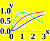
\includegraphics[width=.35cm]{toolb6.png}}
\end{minipage}
}
\newcommand{\toolbV}{
\begin{minipage}[t][1mm][t]{.35cm}{
\vspace*{-8pt}
\includegraphics[width=.35cm]{toolb7.png}}
\end{minipage}
}
\newcommand{\toolbH}{
\begin{minipage}[t][1mm][t]{.35cm}{
\vspace*{-8pt}
\includegraphics[width=.35cm]{toolb8.png}}
\end{minipage}
}
\newcommand{\toolbB}{
\begin{minipage}[t][1mm][t]{.35cm}{
\vspace*{-8pt}
\includegraphics[width=.35cm]{toolb9.png}}
\end{minipage}
}
\newcommand{\toolbQ}{
\begin{minipage}[t][1mm][t]{.35cm}{
\vspace*{-8pt}
\includegraphics[width=.35cm]{toolb10.png}}
\end{minipage}
}
\newcommand{\bigtoolbN}{
\begin{minipage}[t][1mm][t]{.5cm}{
\vspace*{-8pt}
\includegraphics[width=.5cm]{toolb1.png}}
\end{minipage}
}
\newcommand{\bigtoolbA}{
\begin{minipage}[t][1mm][t]{.5cm}{
\vspace*{-8pt}
\includegraphics[width=.5cm]{toolb2.png}}
\end{minipage}
}
\newcommand{\bigtoolbS}{
\begin{minipage}[t][1mm][t]{.5cm}{
\vspace*{-8pt}
\includegraphics[width=.5cm]{toolb3.png}}
\end{minipage}
}
\newcommand{\bigtoolbP}{
\begin{minipage}[t][1mm][t]{.5cm}{
\vspace*{-8pt}
\includegraphics[width=.5cm]{toolb4.png}}
\end{minipage}
}
\newcommand{\bigtoolbD}{
\begin{minipage}[t][1mm][t]{.5cm}{
\vspace*{-8pt}
\includegraphics[width=.5cm]{toolb5.png}}
\end{minipage}
}
\newcommand{\bigtoolbC}{
\begin{minipage}[t][1mm][t]{.5cm}{
\vspace*{-8pt}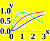
\includegraphics[width=.5cm]{toolb6.png}}
\end{minipage}
}
\newcommand{\bigtoolbV}{
\begin{minipage}[t][1mm][t]{.5cm}{
\vspace*{-8pt}
\includegraphics[width=.5cm]{toolb7.png}}
\end{minipage}
}
\newcommand{\bigtoolbH}{
\begin{minipage}[t][1mm][t]{.5cm}{
\vspace*{-8pt}
\includegraphics[width=.5cm]{toolb8.png}}
\end{minipage}
}
\newcommand{\bigtoolbB}{
\begin{minipage}[t][1mm][t]{.5cm}{
\vspace*{-8pt}
\includegraphics[width=.5cm]{toolb9.png}}
\end{minipage}
}
\newcommand{\bigtoolbQ}{
\begin{minipage}[t][1mm][t]{.5cm}{
\vspace*{-8pt}
\includegraphics[width=.5cm]{toolb10.png}}
\end{minipage}
}
\newcommand{\undock}{
\begin{minipage}[t][1mm][t]{.3cm}{
\vspace*{-8pt}
\includegraphics[width=.3cm]{undock.png}}
\end{minipage}
}
\newcommand{\zoomin}{
\begin{minipage}[t][1mm][t]{.3cm}{
\vspace*{-8pt}
\includegraphics[width=.3cm]{zoom_in.png}}
\end{minipage}
}
\newcommand{\zoomout}{
\begin{minipage}[t][1mm][t]{.3cm}{
\vspace*{-8pt}
\includegraphics[width=.3cm]{zoom_out.png}}
\end{minipage}
}

\newenvironment{rcase}{
\left.\begin{aligned}}
  {\end{aligned}\right\rbrace
}
\newenvironment{lcase}{
\left\lbrace\begin{aligned}}
  {\end{aligned}\right.
}

\maketitle
\vspace{\stretch{.5}}

\newpage

\tableofcontents


\pagebreak

\section*{DAMQT 3.2.0 \label{sec:0}}
DAMQT is a package for the analysis and visualization of the molecular electron density (MED) in 
atoms and molecules, and several related properties like 
density deformations, electrostatic potential, molecular topography, sigma holes, electric field, Hellmann-Feynman forces, 
molecular orbitals and density fingerprints in Zernike-Canterakis and Jacobi functions. 
Furthermore, cluster optimization for non-bonding interacting systems has been recently added to the package.

The method used is based on the DAM\index{DAM} partition of the electron density
into atomic fragments by means of a least
deformation criterion described elsewhere\footnote{For a description of the
fundamentals, see for instance, J. Fern\'andez Rico, et al. Comput. Chem. 25
(2004) 1355; J. Mol. Struct. Theochem 727 (2005) 115, and the references
included in these articles}. On the other hand, density fingerprints are computed
as expansions of Zernike-Canterakis or Jacobi functions inside a ball of user-supplied radius
using translation techniques of Slater or Gaussian basis functions\footnote{For details see G. Urquiza-Carvalho et al. J. Comput. Chem. 39 (2018) 2022}.
Cluster optimization is carried out by means of the EPIC procedure (Gadre S, Babu K Resonance 4 (1999) 40).


In the DAM partition, the electron density of every atomic fragment is expanded in
products of radial factors times regular spherical harmonics centered at its
nucleus. The electron density of the full molecule is thus represented as
a set of atomic expansions in terms of effective 
multipoles, which are functions of the distance to their corresponding nuclei.

% \vspace*{-2cm}
The radial factors of the effective multipoles are piecewise expanded in
terms of exponentials times polynomials of variable $r$. This representation is
used for the fast evaluation of the molecular electrostatic potential (MESP) and field generated by the electron 
density and nuclei, and for the computation of the
Hellmann-Feynman forces on the nuclei as well. The molecular 
topography of MED and MESP, and the atomic and
molecular deformations of density can be also depicted, yielding a
picture that connects with several concepts of the empirical structural
chemistry.

DAMQT has a modular structure in three levels (see fig \ref{fig:1}), with
the interfaces to standard packages for quantum mechanical calculations placed on top. 
In case of ADF, although the interface is available in the suite, we also include it 
as part of DAMQT for completeness. Interfaces to MOLPRO,
GAUSSIAN, MOPAC, TURBOMOLE and NWCHEM are currently included in the package, 
as well as a facility to read MOLEKEL \mkl{ } files.

\begin{figure}[H]
% \hspace*{-0.5cm}
\vspace*{-2cm}
\begin{center}
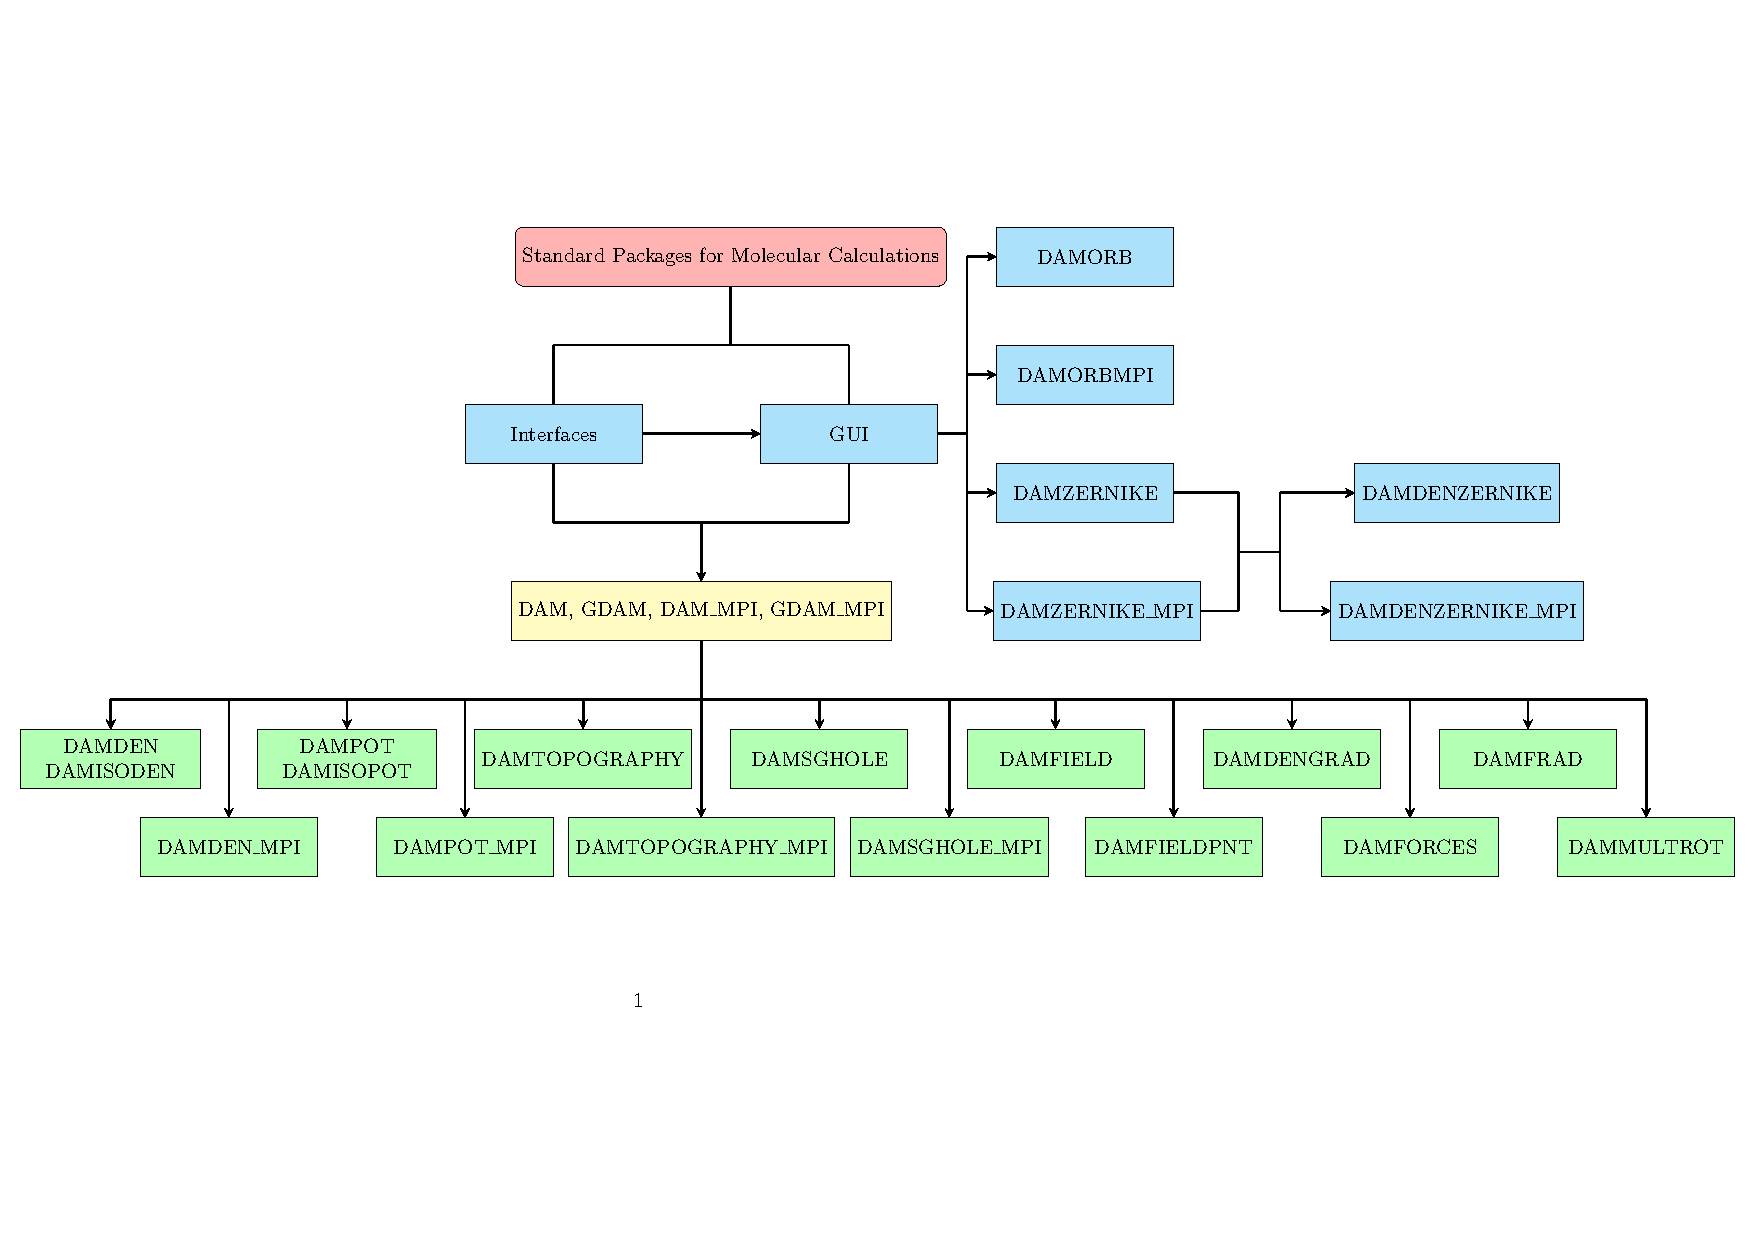
\includegraphics[width=1\linewidth]{DAMQT_structure.pdf}
\end{center}
\vspace*{-2.5cm}
\caption{DAMQT structure \label{fig:1}}
\end{figure}

In this level too, DAMQT includes the GUI\index{GUI} designed to facilitate usage.
This GUI is written in C++ and has been developed using 
Qt library\footnote{The Qt Company, www.qt.io}, 
to facilitate portability between different operating systems.
Also in this level there are some programs available for generating grids of 
molecular orbitals for 2D plotting and 3D visualization with the GUI.
Programs for Zernike-Canterakis or Jacobi expansions
of MED and their grid generation for plotting appear also in this level, as they can be launched from the GUI 
without requiring partition/expansion of MED.
Finally, cluster optimization by EPIC procedure (MESPIMIZER) is implemented within the 3D viewer, albeit
it requires DAM partition/expansion for host molecule. 

Second level corresponds to the programs which carry out the
DAM partition/expansion of density for Gaussian and Slater densities. They are available both for scalar and parallel 
computation with MPI. One of these programs must be run before accessing those of the third level,
because the latter needs the partition/expansion data generated by the former. 

Finally, bottom level contains a variety of programs for computing several properties
using DAM partition/expansion. In particular, this expansion facilitates the effective computation of electron density and its deformations,
electrostatic potential, electric field, density gradient, molecular topography of electron density and electrostatic potential, 
sigma holes and Hellmann-Feynman forces on nuclei.

Unless otherwise explicitly stated, atomic units will be used throughout this
document.

\newpage

\section{Installation \label{sec:1}}

DAMQT 3.2.0 is supplied for Linux and MS Windows under GNU's GPL license. 
The package includes the code sources as well as other ancillary files). 
Sources can be modified and distributed according to GPLv3 terms.

The minimum requirements for installation are 200Mb of RAM memory and 150Mb of
disk storage. Memory requirements strongly depend on the size of the systems to be 
treated. Access to Fortran 90 and C++ compilers and a python interpreter is also required. 

Qt-project's Qt library 5.9 or higher (including development libraries), and OpenGL 3.3 or higher must be installed for the Linux version. 

\texttt{OpenBabel} will be required for cluster optimization using openbabel atom charges.

\texttt{ffmpeg} may be necessary for creating movies from captures.

\subsection{Linux and MacOS installation \label{sec:1.1}\index{installation!linux}}

\texttt{DAM\_3.2.0} is distributed as a tarball ({\it DAM\_3.2.0\_}\texttt{datestamp}{\it .tar.gz}),
where $\texttt{datestamp}$ is an eight-digit date with format \texttt{yyyymmdd}.
To install it in Linux, Unix or MacOS, enter a suitable directory and copy file 
{\it DAM\_3.2.0\_}\texttt{datestamp}{\it .tar.gz}
therein. Extract the content with
\begin{verbatim}
tar -vxzf DAM_3.2.0_datestamp.tar.gz
\end{verbatim}

A directory, \texttt{DAM\_3.2.0}, will be created containing the sources and
ancillary files. \texttt{DAM\_3.2.0} is prepared to be installed with \texttt{cmake},
therefore, check that \texttt{cmake} is already available in your system before starting
installation. It can be very useful to have the graphics interface of 
\texttt{cmake}, named \texttt{cmake-gui}, as it greatly facilitates the handling of
variables setting.

To prevent that files generated by \texttt{cmake} will
be placed in the directory of DAMQT sources, it is highly recommendable
to create a suitable directory and perform installation therein. 

For installation with \texttt{cmake} from the command line, move to the directory
where installation is desired and run either \texttt{cmake} {\it damdir}
(where {\it damdir} is the root directory of DAMQT), or preferably, 
run interactively with \texttt{cmake -i}, for customization options.

By default, \texttt{make install}
will install the package's files in
\texttt{/usr/local/bin}, \texttt{/usr/local/man}, etc (you may need root
privileges for this operation). You can specify an
installation prefix other than \texttt{/usr/local} by setting \texttt{cmake}
variable \texttt{CMAKE\_INSTALL\_PREFIX } to {\it path}, where {\it path} stands for the
desired final location. (WARNING: avoid blank spaces in the pathname).

Many other installation options can be chosen by setting suitable  \texttt{cmake}
variables.

The package can be uninstalled with \texttt{make uninstall}.

In some systems, if \texttt{MESA} library is to be used for OpenGL, it may be 
necessary to run in advance the command:

\texttt{MESA\_GL\_VERSION\_OVERRIDE=4.5 MESA\_GLSL\_VERSION\_OVERRIDE=450} {\it path to DAMQT}

in the console where DAMQT is to be launched. If a version other than 4.5 
(but higher or equal to 3.3) is to be used, modify the command accordingly
(change both 4.5 and 450 in the command).


\subsection{Windows installation \label{sec:1.2}\index{installation!windows}}

MS-Windows version can be also installed with \texttt{cmake}, but 
an autoinstall {\it DAMQT\_3.2.0\_setup.exe} file is also supplied with the package, 
so that you have only to click on this file and follow the installer instructions.

Samples folder will be installed in the {\it AppData/Local} folder.
To prevent unwanted data losses, this folder will not be removed upon uninstalling 
DAMQT. It should be removed by hand if required.

To use cluster optimization with openbabel atom charges, \texttt{OpenBabel} package must be installed
and the pertaining executable must be accessible. Include the directory containing the executable
in the user's \texttt{PATH}, and beware that the \texttt{BABEL\_DATADIR} variable is included
among the user's environment variables. Check that it points to the suitable folder ({\it qeq.txt} file 
must be present therein). An OpenBabel-3.1.1 installer is included in the directory 
{\it windows} of the package for completeness. 

It is important that \texttt{OpenBabel} is installed and the pertaining environment variables set before
launching a DAMQT session for cluster optimization. Otherwise, the executable or some auxiliary files
will not be found and optimization may fail.

To create movies from captures, check that \texttt{ffmpeg} or any other suitable program is accessible by
including the pertining folder in the user's \texttt{PATH} variable. 

\subsection{Starting DAMQT \label{sec:1.3}\index{installation!starting DAMQT}}


\begin{minipage}{.65\linewidth}

To start DAMQT open a {\it console} (UNIX/ linux/ MAC-OS) type \texttt{DAMQT320.exe} and press {\it enter}. 
In case of MS-Windows, the installer allows you to put an icon on the console for direct access.
Alternatively, you can run the DAMQT320.exe in the installation folder.

A pop-up window will appear over a splash image (fig \ref{fig:1_3_1}) 
and you will be asked to select the language. Check the 
option of your choice and press the {\it Start} button. The splash image will glow while  
DAMQT starts. Once the image disappears, DAMQT is ready to work.

\end{minipage}
\begin{minipage}{.38\linewidth}
\vspace*{-8mm}
\begin{figure}[H]
\begin{center}
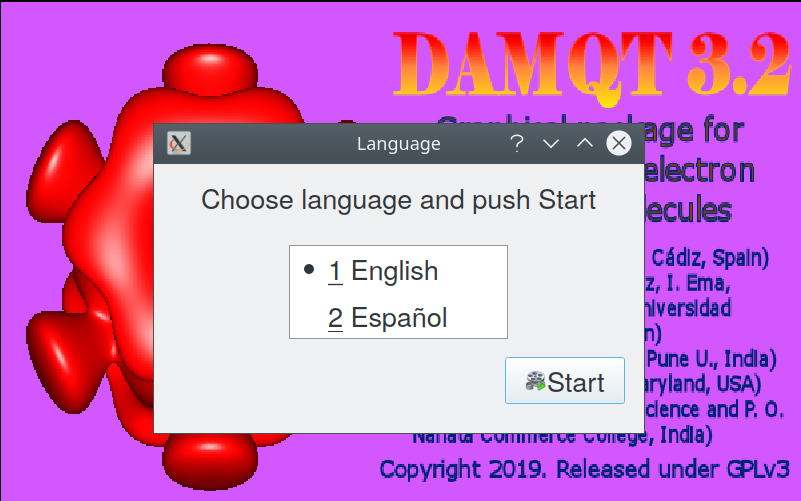
\includegraphics[width=.83\linewidth]{damqt320_splash.png}
\end{center}
\caption{{Starting window}\label{fig:1_3_1}}
\end{figure}
\end{minipage}

\newpage

\section{The Graphical User Interface I: Main window \label{sec:2}\index{main
window}}
The GUI has a standard design with a menu bar and a toolbar on top, an
application driving menu on the left, a display area for applications standard outputs, and
a menu on the right for handling graphical viewers (fig. \ref{fig:2_1}).


\vspace*{0cm}
\begin{figure}[H]
\begin{center}
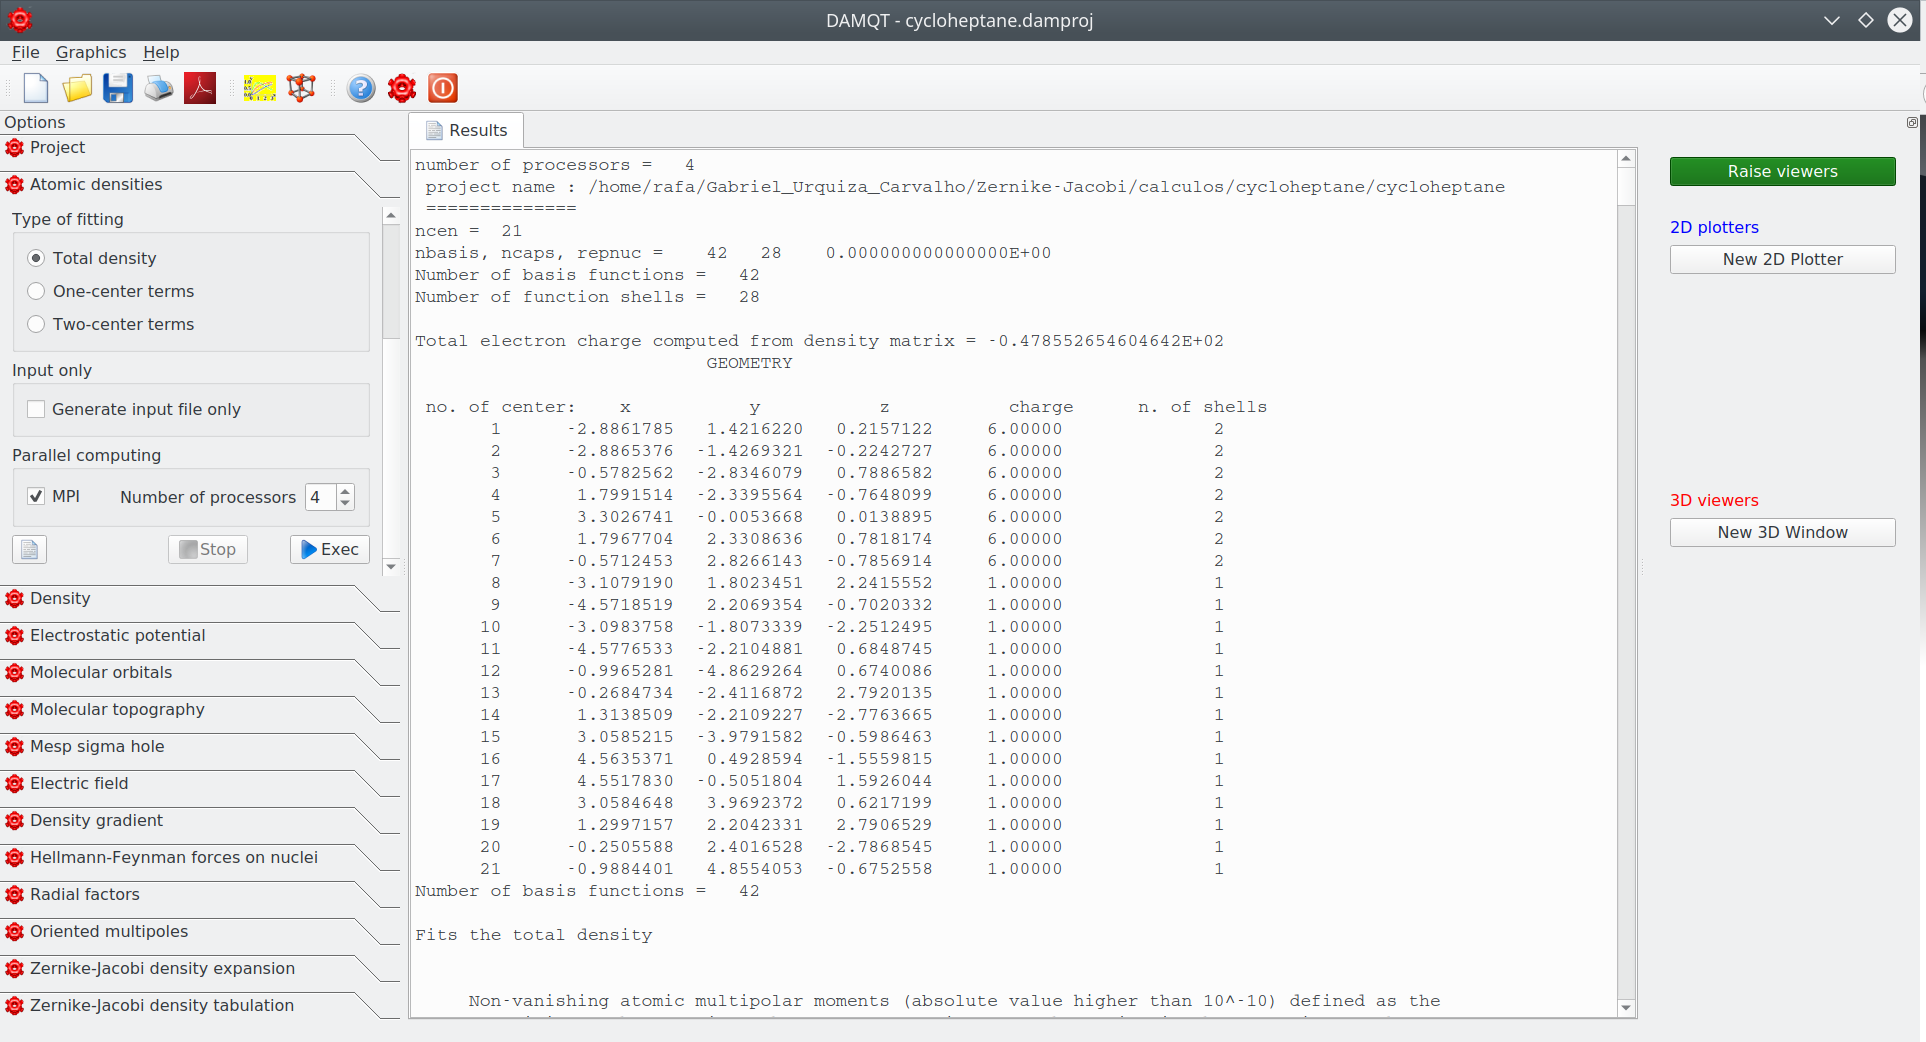
\includegraphics[width=0.5\linewidth]{damqt320_main_panel.png}
\end{center}
\caption{{DAMQT} main window \label{fig:2_1}}
\end{figure}

\vspace*{0cm}
\begin{figure}[H]
\begin{center}

\includegraphics[width=0.5\linewidth]{damqt320_toolbar.png}
\end{center}
\caption{{DAMQT} toolbar \label{fig:2_2}}
\end{figure}

The toolbar\index{toolbar} (fig. \ref{fig:2_2}) contains common options for this
program, namely:


\begin{description}
 \item[\bigtoolbN New file] Clean all options to start working in a new project
 \item[\bigtoolbA Open project] Open an existing  project
 \item[\bigtoolbS Save project] Save the current project
 \item[\bigtoolbP Print] Send the content of the {\it Results} panel to the
selected printer
 \item[\bigtoolbD Pdf file] Print the content of the {\it Results} panel to a pdf
file
 \item[\bigtoolbC 2D viewer] Launch 2D viewer
 \item[\bigtoolbV 3D viewer] Launch 3D viewer
 \item[\bigtoolbH Help] Show this manual
 \item[\bigtoolbB About] Show some information about the program
 \item[\bigtoolbQ Exit] Exit the program
\end{description} 


\vspace*{3mm}

The driving menu on the left of the main window is used for calling the different
modules of DAMQT, and its contents and usage are described in this section.

Graphical tools can be launched from the toolbar or from the menu placed on the right by pressing the 
buttons {\it New 2D Plotter} or {\it New 3D viewer}. When
graphical tools are being used, entries for the currently open 2D and 3D viewers
will be displayed to facilitate navigation through them. Each open viewer has three buttons
labeled as {\it Raise}, {\it Hide}, and {\it Delete}. Pressing the button {\it Raise} the viewer will
be put on top of display. The button {\it Hide} switches between viewer's hide and show states. 
Button {\it Delete} removes the viewer and all its content. The full set of open viewers can be raised
to the foreground by pressing the button labeled as {\it Raise all viewers} on top of the menu.

\subsection{Project \label{sec:2.1}\index{project}}


Every project requires files with data
coming from an LCAO calculation at any level of computation. 
One file is necessary in all cases with
extension \ggbs{}\index{ggbs@\textsl{ggbs} file} (for GTOs) or
\sgbs{}\index{sgbs@\textsl{sgbs} file} (for STO), containing the geometry, nuclear
charges and basis set.
When DAM partition/expansion is required, another file with extension
\den{}\index{den@\textsl{den} file}, must contain the elements of the density
matrix (lower triangle). DAMQT also admits \den{} files compressed with 
gzip\index{gzip} for storage saving (an extension \dengz{} will be expected
in this case) as well as binary files with density sparse matrices containing only non-null elements of the lower triangle with the format $i,j,\rho_{ij}$, the extension in this case being {\it .densprsbin}.

% \vspace*{-5mm}
\begin{figure}[H]
\begin{center}
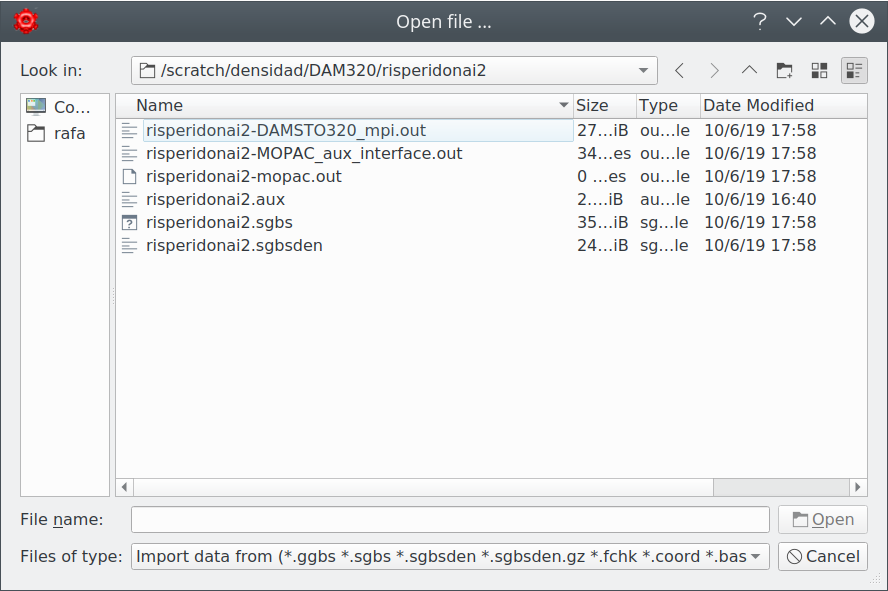
\includegraphics[width=.5\linewidth]{damqt_fig_2_1_1.png}
\end{center}
\caption{Import file navigator \label{fig:2_1_1}}
\end{figure}

Files \ggbs{ }, (\sgbs) and \den{}, {\dengz{} or {\it .densprsbin}} can be loaded by 
supplying their full name (including path) in
the box labeled {\it Import data from}. Alternatively, the name of 
a GAUSSIAN\footnotemark\index{GAUSSIAN} {\it .fchk} file, a
MOLEKEL\index{MOLEKEL}
file {\it .mkl}, a TURBOMOLE\index{TURBOMOLE} basis set, coords or molecular orbitals 
file, {\it .basis}, {\it .coords}, {\it .mos} (they must be renamed to a common name with 
the pertaning extensions), a MOLPRO\index{MOLPRO} output file, {\it .out}, or 
\xml{ } file, a NWCHEM\index{NWCHEM} output file, {\it .nwcout}, a MOPAC\index{MOPAC}
{\it .aux} file, or a PSI4\index{MOPAC} {\it .psiauxden} file
can be supplied. In each case, a suitable built-in
interface\index{interfaces}
included in the package will automatically generate the \ggbs{ } and \den{ }
files from output files of the corresponding package. 
See section \ref{sec:Interfaces} ({\it Interfaces}) in this manual for details.
Pressing the key \teclapuntos, 
a window is displayed for navigating through the directory tree (see fig
\ref{fig:2_1_1}) and selecting any of these files.

\vspace*{5mm}

\begin{minipage}{.35\linewidth}
\vspace*{-2mm}
\begin{figure}[H]
\vspace*{-3mm}
\begin{center}
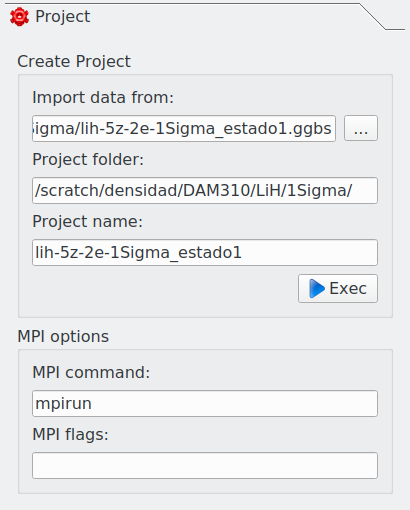
\includegraphics[width=.7\linewidth]{damqt320_project_menu.png}
\end{center}
\caption{Project \label{fig:2_1_2}}
\end{figure}
\end{minipage}
\hspace*{1cm}
\vspace*{5mm}
\begin{minipage}{.45\linewidth}
\begin{table}[H]
\begin{center}
\caption{\label{tab:2.1}Suitable file extensions for running interfaces}
\begin{tabular}{l|c}
interface & extensions \\
\hline
GAUSSIAN & *.fchk \\
MOLEKEL & *.mkl \\
MOLPRO & *.out, *.xml \\
MOPAC & *.aux \\
NWCHEM & *.nwcout \\
PSI4 & *.psiauxden \\
TURBOMOLE & *.basis, *.coords, *.mos \\
\hline
\end{tabular}
\end{center}
\end{table}
\end{minipage}


{\bf WARNING:} the current version of DAMQT only works with {\bf spherical
functions}. This is specially important in case of
Gaussian basis sets, which must be spherical\index{gaussians!spherical}, not
Cartesian\index{gaussians!cartesian}. This implies, for instance,
that if molecular calculations are to be done with GAUSSIAN, the options {\it
5d,7f} must be set in the input file.


Alternatively, the \ggbs{ } and \den{ } files can be hand-written
following the prescription of appendix \ref{A1}. Further interfaces to
other standard packages may be implemented in future versions.

Project files will be allocated in the folder quoted in the {\it Project folder} (see fig \ref{fig:2_1_2}), 
and the application temptatively will assign a name to the project equal to that of the
\ggbs{ } or \sgbs{ } files, but this can be changed by supplying an
alternative name in the box labeled as {\it Project name}.
All the files generated in the project will share the project name, unless
stated otherwise in the modules menus.


To run one of the interfaces, just select a suitable file, according to 
the extensions shown in table \ref{tab:2.1}.
 
\footnotetext{www.gaussian.com}

\begin{center}
\begin{minipage}{.25\linewidth}
\begin{figure}[H]
\begin{center}
\vspace*{-2mm}
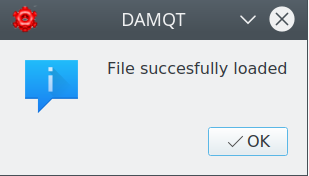
\includegraphics[width=.6\linewidth]{damqt320_info_load.png}
\end{center}
\caption{Project upload \label{fig:2_1_3}}
\end{figure}
\end{minipage}
\begin{minipage}{.25\linewidth}
\begin{figure}[H]
\begin{center}
\vspace*{-2mm}
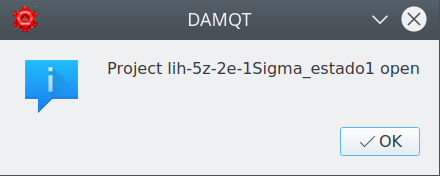
\includegraphics[width=.87\linewidth]{damqt320_info_open.png}
\end{center}
\caption{Project opening\label{fig:2_1_4}}
\end{figure}
\end{minipage}
\end{center}

If an existing \ggbs{ } or \sgbs{ } file is selected, a message
like that shown in fig \ref{fig:2_1_3} confirming or denying the upload will
appear, followed by other confirming project opening (fig \ref{fig:2_1_4}).

Once the required files are found, the key \exec
must be pressed for either building the \ggbs{ } (\sgbs) and \den{ } files with
the interfaces to standard packages or loading them if they already exist. At
the same time, a file with extension \damproj{ }, which contains the default
values for running the remaining modules, will be created. This process must be
carried out at least once for each project. 

To load an existing project, either push the \toolbA icon in the toolbar or,
alternatively, choose the {\it File $\rightarrow$ Open project} option in
top menu, navigate to the desired project and select one of the files displayed.
Recent projects can be directly accessed also from the {\it File} folder in
top menu.

For systems with {\it mpi}, two boxes will appear to
specify the command for executing {\it mpi} programs and  
suitable {\it mpi} flags (see fig \ref{fig:2_1_2}). DAMQT checks if {\it mpirun} or 
{\it mpiexec} commands are installed in the system (in that order), and if any, 
it fills the {\it MPI command} box with the one found in first place.

% \newpage


\subsection{Atomic densities \label{sec:2.2}\index{atomic densities}}

\begin{center}
\begin{minipage}{.59\linewidth}

The tab in the driving menu labeled {\it Atomic densities}, invokes the
DAMSTO or DAMGTO programs which compute the atomic expansion of the density, the
cornerstone of DAMQT partition/expansion, as shown in fig \ref{fig:1}. One of these programs must be run at
least once for every project, except for molecular orbitals plotting, or Zernike-Canterakis or Jacobi
expansions. The package 
includes also a version of these programs for parallel computing with {\it 
mpi}\index{parallel computing}. 

To facilitate the computation in installations where parallel programs only can be 
batch processed, or in case that the user prefers to run the 
programs for density partition and fitting
outside DAMQT environment, an option is available for only generating the input file. 

The exponents and coefficients for the piecewise
representation of the radial factors are stored in a file with extension 
\damqt{ } that will be read by the remaining modules. Figure \ref{fig:2_2_1}
shows the menu displayed when this tab is pressed.

\end{minipage}
\begin{minipage}{.4\linewidth}

\begin{figure}[H]
\begin{center}
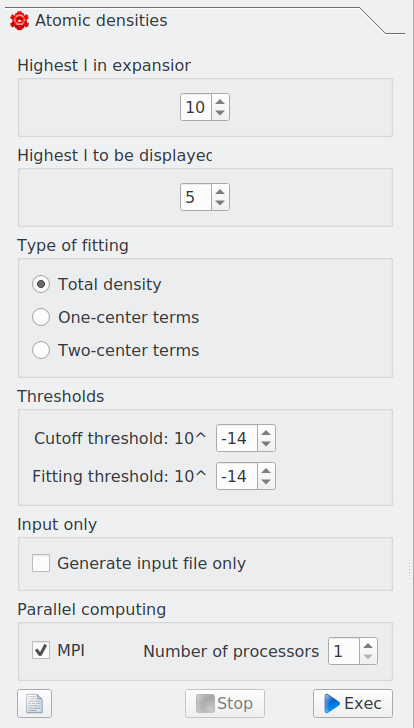
\includegraphics[width=.55\linewidth]{damqt320_atomic_densities.png}
\end{center}
\caption{Atomic densities menu \label{fig:2_2_1}}
\end{figure}

\end{minipage}
\end{center}

The following options can be
set\index{atomic densities!options}:
\renewcommand{\labelitemi}{$-$}
\begin{itemize}
\item {\it Highest l in expansion}: defines the order of the multipole
expansion. Highest allowed value is 25 (default is 10). 
Expansions of the default order yield an absolute error in the atomic
contributions to the density that is estimated to be less than $10^{-5}$ a.u., except in points close
to nuclei, in which around five significant figures are expected to be correct.

\item {\it Highest l to be displayed}: determines the highest order ($l$) of atomic and molecular
multipole components that will be displayed and printed in the output file. It must
be less than or equal to the highest $l$ in the expansion (default is 5).

\item{\it Type of fit\index{atomic densities!type of fit}}: the usual choice 
corresponds to fitting the total
density (default), but representations of only one-center or only two-center
contributions to density in the LCAO framework can be also carried out. In case of 
calculations using the ZDO approximation (MOPAC), the {\it only one-center} option is
automatically set, to keep consistency.

\item{\it Thresholds\index{atomic densities!thresholds}}: threshold for considering
radial factors as negligible ({\it Cutoff}) and for truncation of radial factors 
expansion in Chebyshev polynomials ({\it Fitting}).

\item{\it Input only\index{atomic densities!input only}}: generates the input file 
with the options selected. No partition or fit is actually done.

\item{\it Parallel computing\index{atomic densities!parallel computing}}: for systems 
with {\it mpi} installed, parallel
versions of DAMSTO and DAMGTO can be run. The number of processors can be chosen
and must be lower than or equal to the number of atoms in
the system. This option will remain hidden for systems where {\it mpi} is not
available or in MS-Windows systems. This option is not suitable for running mpi 
batch processes.
\end{itemize}

The key \exec must be pressed to compute the expansion. Besides the \damqt{ },
a file, whose name ends in \dmqtv{ } and which contains auxiliary 
integrals for electrostatic potental computation, will be created. Furthermore, 
some information will be displayed in the standard output
(see fig \ref{fig:2_2_2}). This information includes the
project name, geometry, basis set size, total electron charge retrieved from the density 
(without partition), nonvanishing atomic multipole moments up to the highest order chosen for printing,
and molecular charge and multipoles computed from partition. Notice that, in general,
the multipole order will be lower for printing than for density fitting and computations, i.e.
only a subset of the actually computed and stored multipoles will be printed.
This information is also stored in a file named {\it projectname}-DAMGTO320.out 
for GTO densities,
where {\it projectname} stands for the name of the current project. In case of STO densities,
DAMGTO will be replaced by DAMSTO.

\vspace*{0.3cm}

% \vspace*{-1.cm}
\begin{center}
\begin{tabular}{cc}
\begin{minipage}{.48\linewidth}
\begin{figure}[H]
\begin{center}
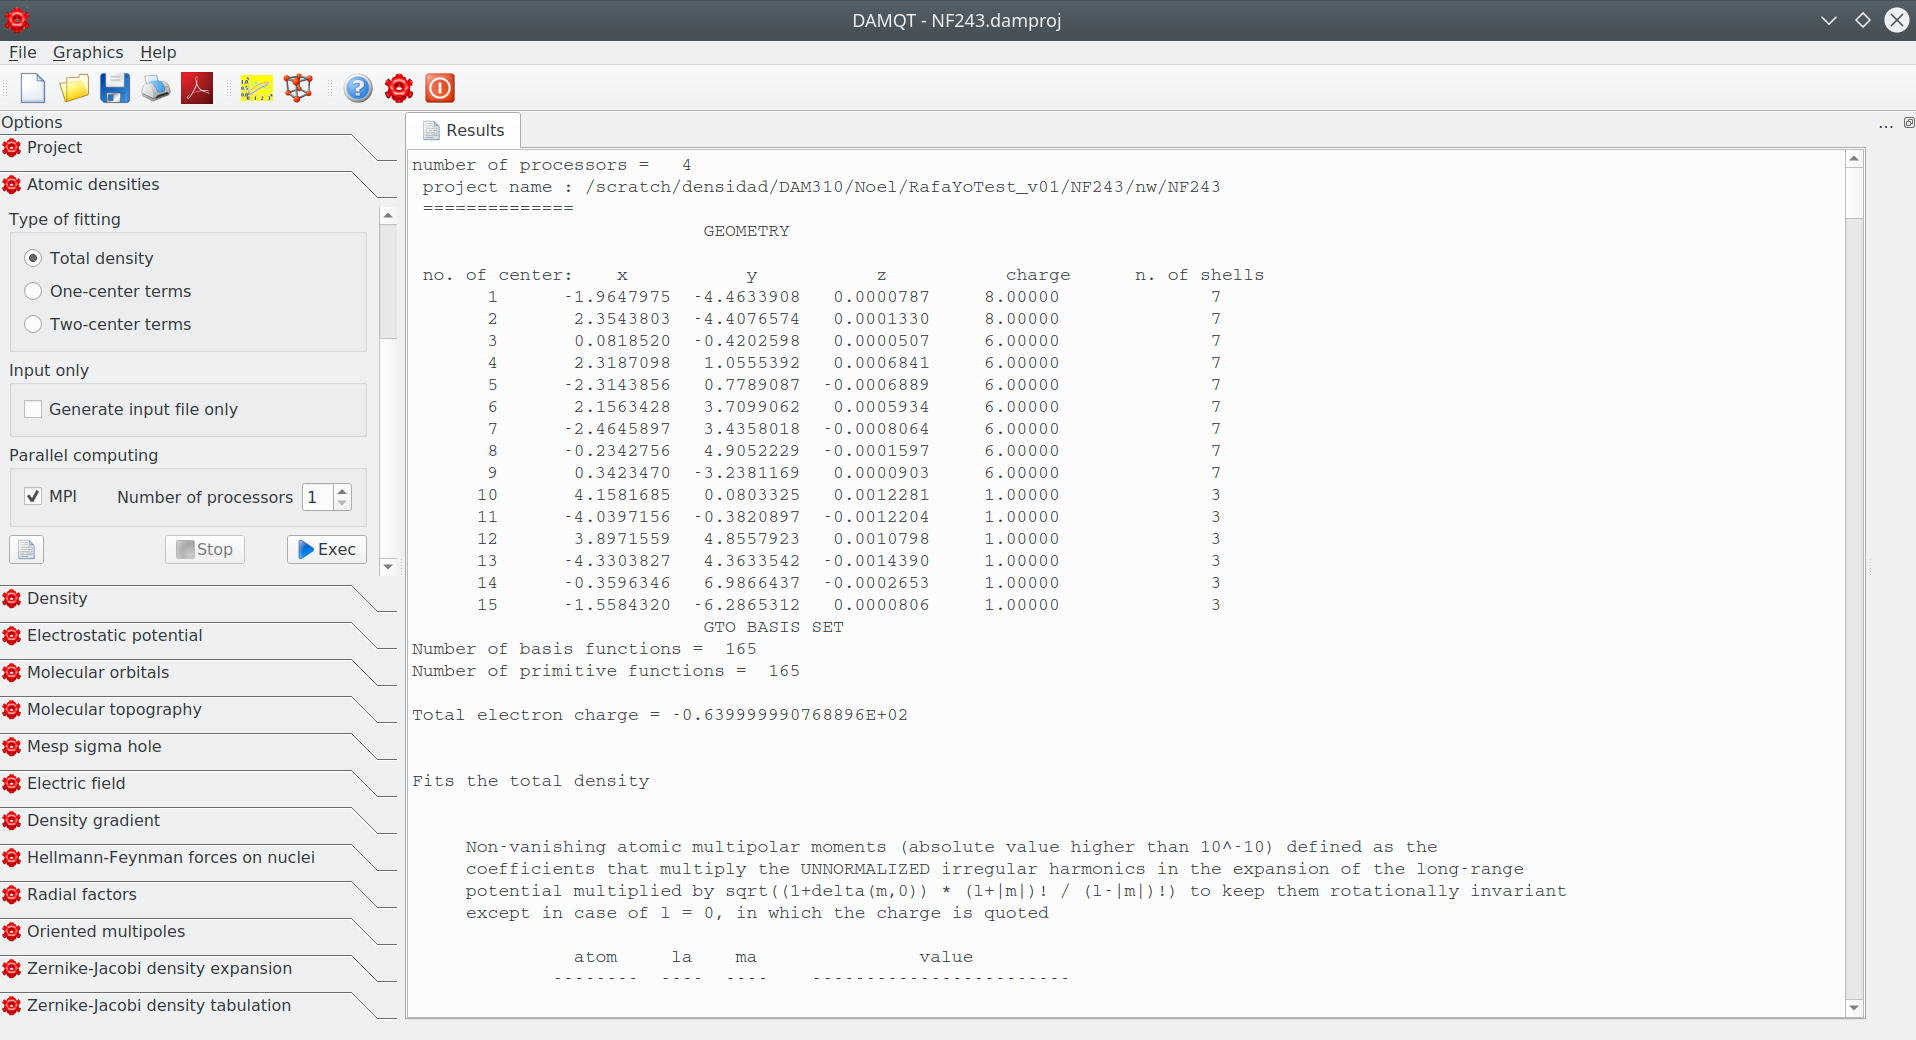
\includegraphics[width=.9\linewidth]{damqt320_standard_output.png}
\end{center}
\caption{{Standard output} \label{fig:2_2_2}}
\end{figure}
\end{minipage}
&
\begin{minipage}{.48\linewidth}
\begin{figure}[H]
\begin{center}
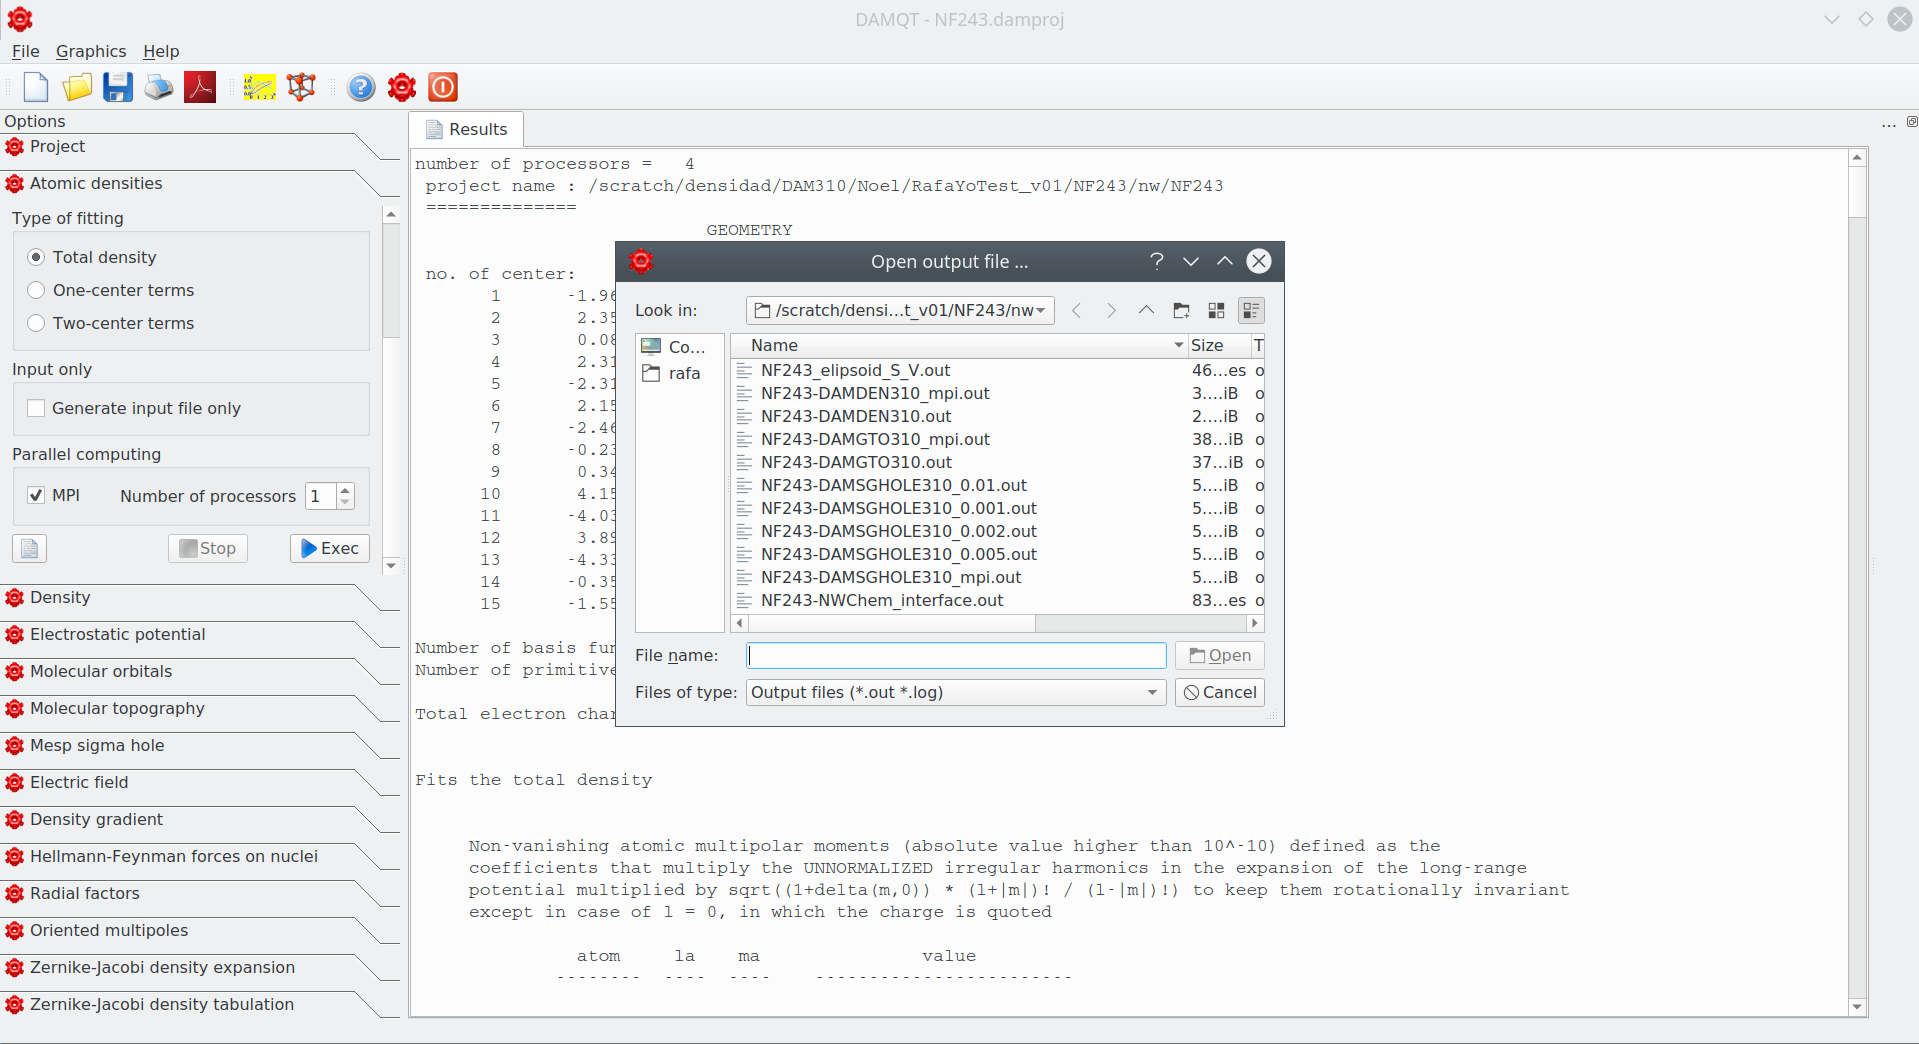
\includegraphics[width=.9\linewidth]{damqt320_output_files_menu.png}
\end{center}
\caption{{Standard output files menu}\label{fig:2_2_3}}
\end{figure}
\end{minipage}
\end{tabular}
\end{center}


Another file with extension {\it .mltmod} containing the moduli of the atomic
multipole moments\index{multipole moments} 
is also generated. The multipole moments are defined
as the coefficients that multiply the {\it unnormalized} irregular spherical harmonics
in the expansion of the long-range potential. Since the moduli of the 
spherical harmonics depend on the value of $|m|$, the values actually stored in file {\it .mltmod}
will be the multipole moments thus defined, $Q_{lm}$, each multiplied by 
$(1 + \delta_{m0}) \; \sqrt{(l+|m|)!/(l-|m|)}!$ to keep
invariance under rotations.

Key \stopkeya enables to stop the process. Key \listados displays a list of all
the currently available \out{ } files (see fig \ref{fig:2_2_3}). The
content of these files can be visualized in the main panel.

% \end{minipage} &

\vspace*{5mm}

\begin{tabular}{lr}
\hspace*{-3mm}
\begin{minipage}{.6\linewidth}

\subsection{Density \label{sec:2.3}\index{density}}

{\it Density} tab gives access to the module for the tabulation of density
and grid generation for 2D contour plots and 3D images (see fig
\ref{fig:2_3_1}).
This module can deal with the density as supplied by any standard package for
molecular calculations ({\it Original density}), i.e. expressed in terms of the
basis set, or with the atomic expansion of the density generated by DAM
({\it Fitted density})\index{density!options}.

When the {\it Original density}\index{density!original} is selected, tabulation
and grid generation can be made only for the full molecular density. The 
{\it Fitted density}\index{density!fitted density} option
(default) opens more possibilities. 
Three options for density are available: {\it Full electron density}\index{density!full electron density} using an expansion 
starting on $l = 0$ and ending at a user-selected $l_{max}$ (lower than or equal to the highest available),
{\it Density deformations}\index{density!density deformations} with an expansion starting in $l = 1$ (i.e. in which the atomic 
spherical terms
have been removed), and {\it Contributions to density}\index{density!contributions to density} corresponding to a user-selected
range of values of $l$.
In each case, the multipole terms to be
included in the atomic expansions can be set with the spinboxes under the label
{\it Atomic terms}, with the pertaining restrictions. 
Results attained with the {\it Full electron density} will be similar to those of the {\it Original
density} option but replacing the original density by its atomic multipole
expansion up to the desired order. When the {\it Highest l} is equal to or higher than
5, the plots obtained in both ways will be indistinguishable.

Choosing {\it Density deformations},
the bond skeleton\index{bond skeleton} of the molecules and some of their 
patterns can be visualized and related with several concepts of the empirical structural chemistry 
such as lone pairs\index{lone pairs}, single, double, triple bonds, electron 
delocalization\index{electron delocalization} and so forth. 

To get smooth 3D surfaces in not very big systems, it is recommended to check the {\it 
gradient}\index{density!gradient} box so that grids with the gradient components are 
computed analytically. This approximately doubles the computational time with respect 
to the computation of density alone. Details on how to get smooth surfaces in big systems 
can be found in section \ref{sec:4.13.10}\index{smooth surfaces}.
 
\end{minipage} &
\begin{minipage}{.4\linewidth}
% \vspace*{-5mm}
\begin{figure}[H]
% \vspace*{-5mm}
\begin{center}
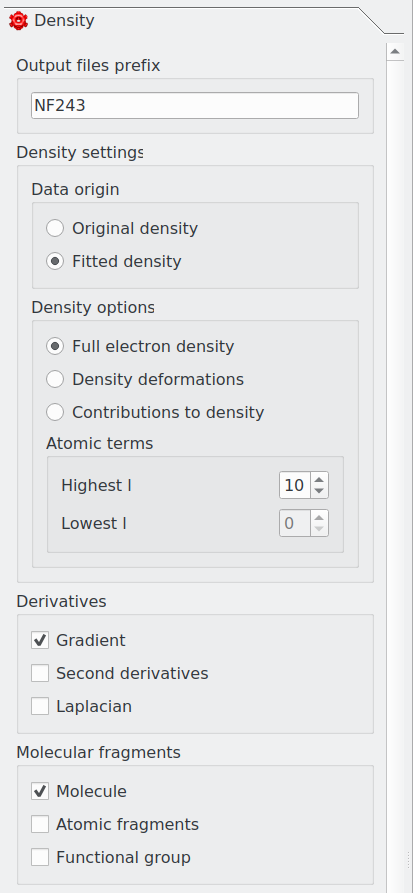
\includegraphics[width=.48\linewidth]{damqt320_density_1.png} \\
\vspace*{-1mm}
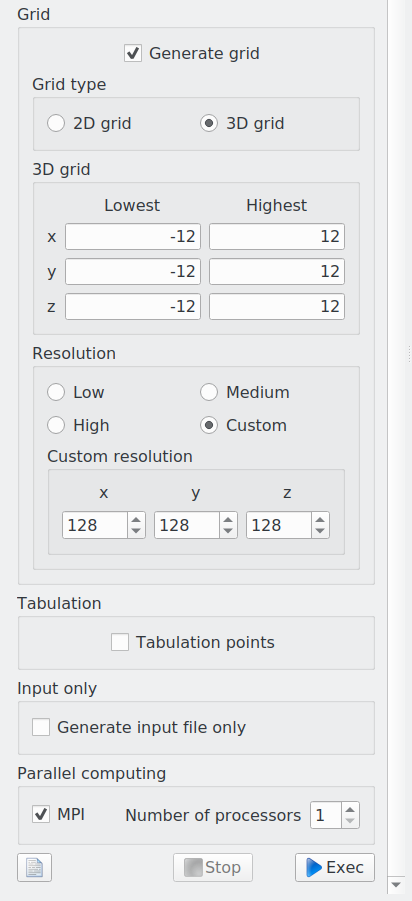
\includegraphics[width=.48\linewidth]{damqt320_density_2.png} \\
\end{center}
\caption{Density menu \label{fig:2_3_1}}
\end{figure} 
\end{minipage}
\end{tabular}

\vspace*{0.5mm}
Furthermore, using the atomic expansion, atomic contributions to density or
atomic deformations\index{atom deformations} can be obtained for single atoms 
or groups of atoms
(functional groups)\index{functional groups}.
Checking the box labeled 
{\it Atomic fragments}, a table is displayed
to select the atoms whose densities or deformations are to be
individually tabulated (see fig \ref{fig:2_3_2}). Checking the box labeled {\it
Functional group}, the density or deformations are tabulated for the 
selected atoms altogether. Indices of centers can be supplied in the box, either separated by commas or 
as ranges specified with the starting and ending indices separated by a hyphen.

The {\it Grid}\index{density!grid} options determine whether a grid for 2D plots
or 3D image of density or deformations will be generated or not.

\begin{tabular}{lr}
\hspace*{-3mm}
\begin{minipage}{.6\linewidth}

If the {\it Generate grid} box is checked (default), and the 2D grid option
selected, a panel like that shown in fig  \ref{fig:2_3_3} is opened for tabulation
settings. 2D grids\index{2D grid!grid definition} are defined in terms of two
variables $u$ and $v$ whose tabulation ranges are supplied in the boxes under
the labels {\it Lowest} and {\it Highest}.

Option {\it Plane} carries out tabulation on a plane. 
Buttons are available to choose $XY$, $XZ$, $YZ$ or arbitrary planes.
Arbitrary plane parameters can be supplied in the suitable boxes which
appear when button labeled {\it Other} is checked.
\end{minipage}
&
\begin{minipage}{.4\linewidth}
\vspace*{-0.3cm}
\begin{figure}[H]
\vspace*{-0.5cm}
\begin{center}
\includegraphics[width=.55\linewidth]{damqt_fig_2_3_2.png}
\end{center}
\caption{Single atom densities \label{fig:2_3_2}}
\end{figure}
\end{minipage}
\end{tabular}

% \vspace*{1.1cm}

\vspace*{1mm}
\begin{tabular}{lr}
\hspace*{-3mm}
\begin{minipage}{.6\linewidth}
Checking option {\it Parametric surface}, tabulation is carried out for a set of
space coordinates $x$, $y$, $z$ computed as functions of $u$ and $v$: $x(u,v)$,
$y(u,v)$, $z(u,v)$. Usual arithmetic operators: $ + $, $ - $, $ * $, $ / $,  
$\hat{ }$, as well as the functions $\sin$, $\cos$, $\tan$, $\log$,  $\ln$, 
$\mbox{abs}$, $\exp$, $\mbox{\\sqrt}$,
can be used to define $x$, $y$, $z$. In this way, a high fexibility in the
choice of 2D surfaces is provided. Three standard resolution levels can be chosen:  {\it
Low} (129x129), {\it Medium} (257x257), or {\it High} (513x513). 
Alternatively, user-supplied resolution can be set pressing the  {\it Custom} button,
in which case a set of spin-boxes will appear to set the resolution in both dimensions.
Numbers introduced in these boxes fix the number of voxels in each direction (i.e.
the number of points minus one). 2D grid tabulated
values are stored in a file with a name starting with the label set in the {\it
Output file prefix} option and with extension \cnt.
Parallel
version of the program is not allowed for 2D grids tabulation.

If the 3D grid option\index{3D grid!grid definition} is chosen (see fig
\ref{fig:19}), the grid will consist of a box with the dimensions of $x$, $y$
and $z$ coordinates supplied in the corresponding boxes under the labels {\it
Lowest} and {\it Highest}, and with the chosen resolution: {\it Low} (65x65x65),
{\it Medium} (129x129x129), or {\it High} (257x257x257). User-supplied resolution is also available.
Grid tabulations are
stored in files with a name starting with the label set in the {\it Output file
prefix} option and with extension \plt. These files are compatible with other
packages for 3D plotting such as
gOpenMol\footnotemark\index{gOpenMol}. For systems with {\it mpi}
installed, parallel computing can be chosen as in case of {\it Atomic
densities}.

To distinguish the different grid files generated (and from those corresponding
to electrostatic potentials) the following naming conventions hold:
\end{minipage}
&
\begin{minipage}{.4\linewidth}

\vspace*{-5mm}
\begin{figure}[H]
\vspace*{-5mm}
\begin{center}
\includegraphics[width=.5\linewidth]{damqt_fig_2_3_3.png}
\end{center}
\caption{2D Grid settings\label{fig:2_3_3}}
\end{figure}

% \vspace*{-5mm}
\begin{figure}[H]
\vspace*{-5mm}
\begin{center}
\includegraphics[width=.5\linewidth]{damqt_fig_2_2_7.png}
\end{center}
\caption{3D Grid settings\label{fig:19}}
\end{figure}
\end{minipage}
\end{tabular}
\vspace*{1mm}

{\it \$fname-d.cnt}: 2D grid tabulation file for the full molecular density or
deformations. \\
{\it \$fname-d-d?.cnt}: 2D grid tabulation files with first derivatives
({\it ?}: $x, y, z$). \\
{\it \$fname-d-d??.cnt}: 2D grid tabulation files with second derivatives 
({\it ??}: $xx, xy, ... zz$). \\
{\it \$fname-d-lplc.cnt}: 2D grid tabulation files with the Laplacian of the
atomic density or deformation. \\
{\it \$fname-d.plt}: 3D grid tabulation file for the full molecular density or selected contributions to density. \\
{\it \$fname-deform-d.plt}: 3D grid tabulation file for the full molecular density deformations. \\
{\it \$fname-cxx-d.plt}: 3D grid tabulation file for the atomic density of {\it xx$^{th}$} center according to the ordering established in
the geometry definition. \\
{\it \$fname-deform-cxx-d.plt}: 3D grid tabulation file for the atomic density
deformation of {\it xx$^{th}$} center according to the ordering established in
the geometry definition. \\
{\it \$fname-frg-d.plt}: 3D grid tabulation file for the density of selected atoms altogether
(functional
group).\\
{\it \$fname-frg-deform-d.plt}: 3D grid tabulation file for the density deformation of selected atoms altogether.\\
{\it \$fname-*-d-d?.pltd}:  3D grid tabulation files with first derivatives of density or deformations
({\it ?}: $x, y, z$). \\
{\it \$fname-*-d-d??.pltd}:  3D grid tabulation files with second derivatives of density or deformations
({\it ??}: $xx, xy, ... zz$). \\
{\it \$fname-*-d-lplc.plt}:  3D grid tabulation files with the Laplacian of the
atomic density or deformations.

{\it \$fname} stands for the root name.

Besides grid generation, molecular density or its deformations can be
tabulated in selected points. This can be done checking the box {\it Tabulation
points} and specifying the points in the table. In this case, the
tabulated values will be printed in the corresponding \out{ } file and displayed
in the main panel.

Options for input file generation and parallel computation are also available like in 
case of density partition and fit.

\subsection{Electrostatic potential \label{sec:2.4}\index{electrostatic
potential}}

\begin{tabular}{lr}
\hspace*{-3mm}
\begin{minipage}{.6\linewidth}
Tab {\it Electrostatic potential} invokes the module for the
tabulation of the electrostatic potential and grid generation for 3D images (see
fig \ref{fig:2_4_1}). Electrostatic potential is computed
using
the density representation. The number of terms included in the expansion is set
with the spinbox labeled {\it Highest l in expansion}. 

Computation using point atomic multipoles can be done checking the box labeled 
{\it Long-range only}\index{electrostatic potential!long-range}; otherwise, a
threshold for long-range is set: the contribution of an atom to the
electrostatic potential in a given point will be computed from the long-range
expansion only if the estimated contribution of the short-range terms is smaller than the
threshold; if it is larger, the radial factors (depending on $r$) will
be used.

For 2D and 3D grid definitions the same comments as in {\it
Density} hold, as well as the same resolution options. 
In particular, to get smooth 3D surfaces in not very big systems, check the {\it 
gradient}\index{electrostatic potential!gradient} box so that grids with the gradient 
components are computed analytically. This approximately doubles the computational time 
with respect to the computation of electrostatic potential alone. For smooth surfaces in big systems see section \ref{sec:4.13.10}\index{smooth surfaces}.

For systems with {\it mpi} installed, parallel computing can be chosen as in 
case of {\it Atomic densities}.

File names follow a convention analogous to that mentioned
in case of density. Thus, grid files\index{electrostatic potential!grid} are
named {\it \$fname-p.plt}, files with first derivatives of the potentials
are named {\it \$fname-p-d?.pltd}, and so forth. Root name {\it \$fname} can be
set in the {\it Output file prefix} box. These files are also
compatible with gOpenMol.

Options for input file generation and parallel computation are also available.
\end{minipage}
&
\begin{minipage}{.4\linewidth}

\begin{figure}[H]
\begin{center}
\vspace*{-5mm}
\includegraphics[width=.65\linewidth]{damqt_fig_2_4_1.png}
\end{center}
\caption{Electrostatic potential \label{fig:2_4_1}}
\end{figure}
\end{minipage}
\end{tabular}
\vspace*{0.1mm}
\footnotetext{www.csc.fi/gopenmol/}


\subsection{Molecular orbitals \label{sec:2.5}\index{molecular orbitals}}

Tab {\it Molecular orbitals}\index{molecular orbitals} creates 
2D and 3D grids for plotting molecular orbitals (fig
\ref{fig:2_5_1}). For options and grid definitions, same comments as in sections
\ref{sec:2.3} and \ref{sec:2.4} hold. Indices of molecular orbitals to be
plotted are given, separated by commas, in the box labeled {\it Molecular
orbitals}. Ranges of indices can be defined using hyphens as separators.

Molecular orbitals are sorted on ascending energy. In case of UHF calculations with 
MOLPRO, different sets of orbitals are obtained depending on the interface used. See 
section \ref{sec:5.2} for details.


\subsection{Molecular topography \label{sec:2.6}\index{molecular topography}}

Tab {\it Molecular topography}\index{molecular topography}
is intended for mapping of critical points (CPs)\index{molecular topography!critical points}, 
determination of molecular graph\index{molecular topography!molecular graph} and computation of 
atomic basin borders\index{molecular topography!atomic basin}
for both electron density and electrostatic potential (fig \ref{fig:2_6_1}). Mapping of all the critical points is the 
first step required for any further calculation {\it viz.} determination of molecular graph and atomic basins.

\vspace*{10mm}

\begin{tabular}{lcr}
\begin{minipage}{.53\linewidth}
\begin{figure}[H]
\begin{center}
\vspace*{-6.4mm}
\includegraphics[width=.45\linewidth]{damqt_fig_2_5_1.png}
\end{center}
\caption{{Molecular orbitals}\label{fig:2_5_1}}
\end{figure}
\end{minipage}
&
\begin{minipage}{.47\linewidth}
\begin{figure}[H]
\begin{center}
\vspace*{-8mm}
\includegraphics[width=.52\linewidth]{damqt_fig_2_6_1a.png}
\includegraphics[width=.52\linewidth]{damqt_fig_2_6_1b.png}
\end{center}
\caption{Molecular topography \label{fig:2_6_1}}
\end{figure}
\end{minipage}
\end{tabular}

\vspace*{5mm}
The values of density (MED) and electrostatic potential (MESP), their gradient and second derivatives are calculated while 
finding the CPs using DAM partition/expansion method. 
The number of terms included in the expansion 
for calculation of field values can be set with the spinbox labeled {\it Highest l in expansion}. 
The guess points required for initiating the search of critical points are determined internally. 
However, especially in case of electrostatic potential, where CPs can be located far from molecular skeleton, 
guess point generation requires gradient evaluation on a grid. The size of the grid and step-size can be altered
under the option {\it Guess points} by mentioning the optimal {\it Box size} and {\it Step size} in atomic units.
User may intuitively provide additional guess points, if required, by checking {\it Add guess points for CPs}. The points can be 
supplied in a pop-up table or, alternatively, in an external text file, whose record must contain values of 
$(x,y,z)$ coordinates of the points (one point per line). 

These guess points are optimized to critical points using L-BFGS subroutine, an iterative method for solving
unconstrained nonlinear optimization problems. The search of a critical point starting from the guess point 
is performed within a cubical region around latter. A cube of side ranging $0.5-1.0 \;$a.u. is 
recommended for this purpose. The control over the size of this cube is provided under the option {\it Box margins size}
which appears on checking the {\it map critical points} option. A convergence threshold is required for determining if the 
program has reached the critical point. It is optimal to provide lower value of threshold for electron density than
electrostatic potential {\it e.g.} $4 \cdot 10^{-16}$ and $4 \cdot 10^{-12}$ respectively.  

Molecular graph for MED and MESP-based topograph is calculated 
using the option {\it Gradient path}\index{molecular topography!gradient path}. 
This primarily requires the file containing the critical points to start the calculation. 
Absence of CP file will automatically instruct to perform the mapping of critical points. 
The gradient paths leading to asymptote requires to be bound by a large box of recommended side length of 5.0 a.u. 

Atomic basins\index{topography!atomic basins} for MED and MESP are 
calculated under the option {\it Atomic basin}. This computation requires  
the file containing the CPs and the determination of molecular graph. Checking the {\it compute basin} option,
automatically checks the option of {\it gradient path}. The appearance of the basin can be corrected by checking 
the {\it Extra connections} box,
and setting the {\it Connection threshold} value. 
The greater the value, the higher the number of connecting lines appearing in the basin.


\vspace*{5mm}
\begin{tabular}{lr}
\hspace*{-3mm}
\begin{minipage}{.6\linewidth}

The files containing critical point are named {\it \$fname-cps-d.xyz} and {\it \$fname-cps-v.xyz}, depending on whether they store
MED CPs or MESP CPs respectively. Corresponding files with name {\it \$fname-cps-d.eigv} or {\it \$fname-cps-v.eigv} 
contain eigenvector information in the same order of CPs mentioned in the file containing CPs. The files containing molecular 
graph 
information are stored in {\it \$fname-d.gpdat} or {\it \$fname-v.gpdat}. 
In case of atomic basins, the surfaces 
are stored in {\it \$fname-d.basins} or {\it \$fname-v.basins}.

Options for input file generation and parallel computation are also available.

\subsection{MESP sigma hole \label{sec:2.7}\index{MESP sigma hole}}

Tab {\it MESP sigma hole} handles the module for the computation of
molecular electrostatic potential (MESP) on an isosurface of density (MED) (fig \ref{fig:2_7}). 
The values of MESP at the vertices of the triangles 
in which the MED isosurface is decomposed are stored in a file with extension $.sgh$. 
Furthermore local maxima (minima) higher (lower) than a given threshold are searched. The 
threshold is set as a fraction of the absolute extrema values in the box labeled {\it Threshold 
for local extrema}. The default value is 0.90 (90\% of the absolute extrema values). 
A histogram\index{MESP sigma hole!histogram} of 
MESP on the surface (area vs MESP values) is also computed. 
The histogram is a plot of the surface area (in bohr$^2$) vs the MESP value, and can be used as a tool for comparing {\it sigma holes}
of different molecules. 

\end{minipage}
&
\begin{minipage}{.4\linewidth}
\begin{figure}[H]
\begin{center}
\vspace*{-0.5mm}
\includegraphics[width=.8\linewidth]{damqt320_mesp_sg_hole.png}
\end{center}
\caption{{MESP sigma hole}\label{fig:2_7}}
\end{figure}
\end{minipage}
\end{tabular}

\vspace*{0.3mm}

To compute the sigma hole, the MED must be previously tabulated on a 3D grid (see sec \ref{sec:2.3}), and the pertaining $.plt$ 
file must be chosen in the box labeled as {\it Import density grid from}. 
The MED value for isosurface can be set in the box labeled as {\it Density value}.
Three thresholds can be set in the corresponding boxes: for geometry (two points are considered the 
same if they are separated a distance lower then this threshold), for MESP long-range (short-range 
contributions are not computed when they are lower than it), and for local extrema. MESP can be 
computed from the DAM expansion of density (preferable) or, checking the
box labeled as {\it Exact potential}\index{MESP sigma hole!exact potential}, directly from density 
matrix and basis set without using the DAM expansion. Computation of exact potential is very much 
slower than computation from DAM expansion, and is only recommended for testing purposes. 

A spectrogram of the MESP on the surface and the local extrema can be displayed with the 3D viewer 
included in the suite  --see sec \ref{sec:4.13.7}-- and the histogram can be displayed with the built-in 2D plotter --see sec \ref{sec:3.3}.

The program also provides statistics on MESP: average values (positive, negative and total MESP), 
variances, mean deviation and $\nu$ parameter, introduced by P. Politzer, J.S. Murray et al.\footnote{P.P. Politzer, P. Lane, J.S. Murray and T. Brink, J.. Phys Chem., 96, 7938 (1992); J.S. Murray, P. Lane, T. Brink and P. Politzer, {\it ibid}, 97, 5144 (1993)}

Main results of MESP statistics are collected in a file with a name appended with 
\texttt{\_SGMESP\_summary.txt}, whose content is described in appendix \ref{A5}.


\vspace*{5mm}
\begin{tabular}{lr}
\hspace*{-3mm}
\begin{minipage}{.5\linewidth}
\begin{figure}[H]
\begin{center}
\vspace*{-0.5mm}
\includegraphics[width=.4\linewidth]{damqt_fig_2_8_1a.png} \\
\includegraphics[width=.4\linewidth]{damqt_fig_2_8_1b.png} \\
\includegraphics[width=.4\linewidth]{damqt_fig_2_8_1c.png}
\end{center}
\caption{{Electric field}\label{fig:2_8}}
\end{figure}
\end{minipage}
\begin{minipage}{.5\linewidth}
\begin{figure}[H]
\begin{center}
\vspace*{-0.5mm}
\includegraphics[width=.45\linewidth]{damqt_fig_2_9_1a.png} \\
\includegraphics[width=.45\linewidth]{damqt_fig_2_9_1b.png}
\end{center}
\caption{{Density gradient}\label{fig:2_9}}
\end{figure}
\end{minipage}
\end{tabular}

% \vspace*{5mm}


\subsection{Electric field \label{sec:2.8}\index{electric field}}

Tab {\it Electric field} manages the module for the computation of
electric field lines\index{electric field!lines} from the atomic multipole expansion (fig \ref{fig:2_8}).
The computation is made in points separated by user-supplied steps along each
selected line. 
This module also computes 2D atomic basins\index{electrostatic potential!2D basins} of electrostatic potential in molecular 
symmetry planes, provided that the critical points of electrostatic potential have been previously computed in the {\it Molecular 
topography} module.

% \vspace*{0.5mm}
% \begin{tabular}{lr}
% \hspace*{-3mm}
% \begin{minipage}{.6\linewidth}

Boxes labeled {\it Highest
number of lines} and {\it Highest number of points} are used to set
the maximum number of lines and points per line to be evaluated, and step size is
set in the box labeled {\it Stride length}. The size of the space region in which
lines will be computed is defined in the same way as employed for defining the
3D grid dimensions in the {\it Density}  and {\it Electric field} modules.
The {\it Set of starting directions} of lines can be chosen among the following choices, 
all of them based on icosahedron vertices and symmetry axes:
$(0)$ no automatic direction,
$(1)$: vertices (12 directions per nucleus), $(2)$: C3 axes (20), $(3)$: C2 axes (30),
$(4)$: vertices + C3 (32), $(5)$ vertices + C2 (42), $(6)$ C3 + C2 (50), and
$(7)$: vertices + C3 + C2 (62).

In 2D grids, the option for set of starting directions is replaced by the {\it Number of lines per nucleus}.

% \newpage

When the box {\it Extra lines} is checked, additional directions can be given in a pop-up table built in the GUI or read from an 
external file both in 3D and 2D grids. Checking the box labeled {\it Add starting points to table} triggers the pop-up table 
display, and the external text file can be specified in the box labeled {\it Read file
from}. In 3D grids, this file must contain one record per line to be plotted
with the starting point of the line specified as (free format):

\begin{verbatim}
ICEN    X    Y    Z   
\end{verbatim}

where ICEN is an integer with the index of the nucleus from which the line
departs. A negative or zero value means a line starting from a point that
is not a nucleus.

X, Y and Z are real numbers whose meaning depends on whether
the line departs from a nucleus or not. For a line starting at a nucleus, they
define the departure direction of the line. For a line which does not start in a
nucleus, they just define the starting point of the line.

In 2D grids, the format is:

\begin{verbatim}
ICEN    U    V   
\end{verbatim}

with the same meaning of ICEN as before, and
where U and V are the corresponding 2D coordinates.

Selection of zero lines per nucleus is allowed to generate 2D basins without field lines for further 2D plotting.


\subsection{Density gradient \label{sec:2.9}\index{density gradient}}

Tab {\it Density gradient} handles the module for the computation of
density gradient lines\index{density gradient!lines} from the atomic multipole expansion (fig \ref{fig:2_9}).
The computation is made in points separated by user-supplied steps along each
selected line. 
This module also computes 2D atomic basins\index{density!2D basins} of electron density in molecular symmetry planes provided that 
the critical points of electron density have been previously computed in the {\it Molecular topography} module.
 

\vspace*{1mm}
\begin{tabular}{lr}
\hspace*{-3mm}
\begin{minipage}{.6\linewidth}

Same comments as in electric field section hold in this case too for options
and for 2D borders of basins.

\subsection{Hellmann-Feynman forces on nuclei
\label{sec:2.10}\index{Hellmann-Feynman!forces}}

Tab {\it H-F  forces on nuclei}\index{forces} invokes the module for
the computation of the Hellmann-Feynman forces on the nuclei of the molecule
(fig \ref{fig:2_10}).

DAM\index{DAM} partition of the density
facilitates a decomposition of the total HF force on a nucleus into
internal\index{forces!internal} and external\index{forces!external} contributions. 
The former correspond to the force
exerted on the nucleus of a given atom by its own electron cloud, and the
latter to the force exerted by the nuclei and clouds of the remaining atoms.

\end{minipage}
&
\begin{minipage}{.4\linewidth}

\vspace*{-1.0cm}
\begin{figure}[H]
\begin{center}
% \vspace*{-5mm}
\includegraphics[width=.7\linewidth]{damqt_fig_2_10.png}
\end{center}
\caption{H-F forces\label{fig:2_10}}
\end{figure}
\end{minipage}
\end{tabular}
\vspace*{1pt}

Notice that for a molecule in the equilibrium geometry, 
total forces\index{forces!total} on nuclei
must be zero {\it provided that the wavefunction fufills the
conditions for the Hellmann-Feynman theorem\index{Hellmann-Feynman!theorem} to
be applicable (Berlin's conditions\footnotemark
\index{Hellmann-Feynman!theorem!fulfillment}}).
Wavefunctions which do not fulfill the theorem yield 
spurious\index{forces!spurious} force contributions due to the lack of
fulfillment. 
In particular, nonphysical components leading to translation and
rotation of the molecule as a whole ({\it perpetuum mobile}) may appear.

\footnotetext{Berlin T J Chem Phys 19 (1951) 208}

DAMQT enables filtering of these spurious components by decomposing the total forces
into {\it conformational forces}\index{forces!conformational}
(physically meaningful) , and 
{\it nonconformational forces}\index{forces!nonconformational} (physically meaningless).
The latter terms may be used as a hint on the degree of fulfillment of the HF
theorem by the wavefunction, in the sense that high spurious forces imply a
low degree of fulfillment. 

However, low spurious forces do not necessarily
imply a high degree of fulfillment; in this case the degree of fulfillment
should be established by other procedures.
Forces are stored in a file with extension {\it .forces}.

Besides these files, detailed information about the electrostatic
potential\index{electrostatic potential!values on nuclei}, electric 
field\index{electric field!values on nuclei} and forces on the
nuclei\index{forces!values on nuclei} is given in the standard output (main panel)
and stored in a file with the name ended in DAMFORCES320.out.

If the {\it Atoms} option is checked, individual atoms can be selected
(see fig \ref{fig:2_10}) for a more detailed information about the forces
acting
on their nuclei. In particular, the contributions of every atom to the external
forces on the selected nuclei are given.


\subsection{Radial factors \label{sec:2.11}\index{radial factors}}

Tab {\it Radial factors}\index{radial factors} handles the module for
tabulating the radial factors selected (fig \ref{fig:2_11}). Tabulation points
$r$
are defined in an interval with user-defined starting and ending points and
separated by the selected step. Further individual values of $r$ can be added to
the set by checking the box {\it Extra values}. A table will open where these values can be included.

Centers whose radial factors
will be tabulated can be entered in the bottom box. Indices of individual centers must be separated by commas, and indices ranges can be defined with hyphens. 
First and second derivatives of radial factors can be also computed by 
checking the respective boxes.

\begin{tabular}{lcr}
\hspace*{-3mm}
\begin{minipage}{.3\linewidth}
\begin{figure}[H]
\begin{center}
\includegraphics[width=.7\linewidth]{damqt_fig_2_11.png}
\end{center}
\caption{{Radial factors}\label{fig:2_11}}
\end{figure}
\end{minipage}
&
\begin{minipage}{.3\linewidth}
\begin{figure}[H]
\begin{center}
\vspace*{5mm}
\includegraphics[width=.74\linewidth]{damqt_fig_2_12_1.png}
\end{center}
\vspace*{1.5cm}
\caption{{Oriented multipoles menu}\label{fig:2_12_1}}
\end{figure}
\end{minipage}
&
\begin{minipage}{.3\linewidth}
\vspace*{5mm}
\begin{figure}[H]
\begin{center}
\includegraphics[width=1.22\linewidth]{damqt_fig_2_12_2.png}
\end{center}
\vspace*{1.cm}
\caption{{Oriented multipoles frame}\label{fig:2_12_2}}
\end{figure}
\end{minipage}
\end{tabular}

\subsection{Oriented multipoles \label{sec:2.12}\index{oriented multipoles}}

Tab {\it Oriented multipoles}\index{oriented multipoles} invokes the
module for locally reoriented multipoles (fig \ref{fig:2_12_1}). These
reoriented multipoles can be useful to quantify charge delocalization over a set
of atoms. The atomic multipole components of density of a given group of atoms
are rotated from the molecular frame, with $x$, $y$ and $z$ axes, to a new frame
whose $z'$ axis is perpendicular to the plane defined by three selected atoms,
$(C_1,C_2,C_3)$, and the new $y'$ axis lies in the bisector of the angle
$\widehat{C_1C_2C_3}$ (see fig \ref{fig:2_12_2}).


\subsection{One-center MED expansions in Zernike-Canterakis or Jacobi functions \label{sec:2.13}\index{Zernike-Jacobi}}

Tab {\it Zernike-Jacobi expansion}\index{Zernike-Jacobi expansion} computes a one-center expansion
of MED inside a ball centered at the positive charges center of the system
in terms of Zernike-Canterakis or Jacobi functions (see fig
\ref{fig:2_13}). The expansion 
coefficients, $\Omega_{kl}^m$ can be used to build
rotationally invariant fingerprints, $F_{kl}$, of MED:
% 
$$ 
F_{kl} = \sqrt{ \sum_{m=-l}^l (\Omega_{kl}^m)^2 } 
$$
%
which can be used for molecular pattern-recognition. The coefficients $\Omega_{kl}^m$ are stored in files
with extension {\it .zernike} or {\it .jacobi} depending on the type of expansion.
The fingerprints $F_{kl}$ are printed in the output file.


% \begin{tabular}{lr}
% \hspace*{-3mm}
% \begin{minipage}{.6\linewidth}
   
\begin{tabular}{lr}
\begin{minipage}{.5\linewidth}
\vspace*{-15mm}
\begin{figure}[H]
\begin{center}
\vspace*{4cm}
\includegraphics[width=.5\linewidth]{damqt_fig_2_13.png}
\end{center}
\vspace*{2.4cm}
\caption{{Zernike-Jacobi expansion}\label{fig:2_13}}
\end{figure}
\end{minipage}
&
\begin{minipage}{.5\linewidth}
\begin{figure}[H]
\begin{center}
\vspace*{0mm}
\includegraphics[width=.5\linewidth]{damqt_fig_2_14_1.png}
\end{center}
\vspace*{0cm}
\caption{{Zernike-Jacobi tabulation}\label{fig:2_14_1}}
\end{figure}
\end{minipage}
\end{tabular}
\vspace*{1cm}

The ball radius, and expansion type and length can be set by the user, as well as
cutoffs for displaying multipoles and neglecting charge densities in the expansion.
The ball radius can be supplied as an absolute value or as an increase over the distance
of the farthest nucleus to the ball center. In this case, the {\it Relative} button must be 
checked. The expansion lenght involves two indices: the $l$ index corresponding to the spherical harmonics
taken in the expansion, and the $k$ index labeling the functions for each $l$. The boundaries of these
indices can be taken as independent from each other (default), or in an echelon form:
$k_{top}(l) = k_{max} - l$, if the pertaining button is checked.

As the translation techniques implemented involve a one-dimension numerical integration
(quadrature) in the variable $r$, the size of this quadrature can be set by user.

\begin{tabular}{lcr}
\begin{minipage}{.3\linewidth}
\begin{figure}[H]
\begin{center}
\vspace*{0mm}
\includegraphics[width=.7\linewidth]{damqt_fig_2_14_2.png}
\end{center}
\vspace*{8mm}
\caption{{Choose $l$ option}\label{fig:2_14_2}}
\end{figure}
\end{minipage}
&
\begin{minipage}{.3\linewidth}
% \vspace*{-0.7cm}
\begin{figure}[H]
\begin{center}
\vspace*{0mm}
\includegraphics[width=.75\linewidth]{damqt_fig_2_14_3.png}
\end{center}
\caption{{Choose $(l,k)$ option}\label{fig:2_14_3}}
\end{figure}
\end{minipage}
&
\begin{minipage}{.3\linewidth}
\begin{figure}[H]
\begin{center}
\vspace*{3mm}
\includegraphics[width=.75\linewidth]{damqt_fig_2_14_4.png}
\end{center}
\caption{{Choose $(l,k,m)$ option}\label{fig:2_14_4}}
\end{figure}
\end{minipage}
\end{tabular}

\subsection{Zernike-Jacobi density tabulation\label{sec:2.14}\index{Zernike-Jacobi density tabulation}}

{\it Zernike-Jacobi density tabulation} tab gives access to the module for the tabulation of density
computed with Zernike-Canterakis or Jacobi expansions inside a ball.
Grids of the density thus computed can be generated for 2D contour plots and 3D images (see fig
\ref{fig:2_14_1}) that can be visualized in the 2D plotter and the 3D viewer. 

Indices for projection can be selected in different ways. When the option {\it Choose all functions} is selected,
all the functions available for projection can be chosen in the selected ranges of $l$ and $k$ indices, fixed in
the pertaining spin boxes. Alternatively, option {\it Choose l index} selects individual values or
ranges of $l$ index, with all values of $k$ and $m$ indices compatible (see fig \ref{fig:2_14_2}). Commas are used as separation 
character 
and hyphens are used for ranges. Option {\it Choose k index} is likewise but for $k$ index.
Finally, individual pairs of $(l,k)$ values (with all $m$ compatible) and triads of $(l,k,m)$ can be selected 
in the last two options (see figs \ref{fig:2_14_2} and \ref{fig:2_14_4}). In these cases, parenthesis are just optional cosmetic
aids to help in identifying pairs or triads, but are removed when generating input files.

\newpage

\section{The Graphical User Interface II: 2D Plots \label{sec:3}}

DAMQT has its own 2D plotter\index{2D plotter} built in the GUI\index{GUI}. The plotter can be launched by either pressing the 
key \bigtoolbC in the toolbar, by choosing {\it Graphics $\rightarrow$ 2D Viewer} in the upper menu
or by pressing the button labeled as {\it New 2D plotter} on the right menu. 
A 2D viewer will be displayed on top of the display, as shown in fig \ref{fig:3_1}. 
   
\vspace*{5mm}

\begin{figure}[H]
\begin{center}
\vspace*{0mm}
\includegraphics[width=.5\linewidth]{damqt320_2D_start_window.png}
\end{center}
\vspace*{0cm}
\caption{{2D viewer window}\label{fig:3_1}}
\end{figure}

\vspace*{1cm}

New 2D viewers can be launched without running any DAMQT application and several viewers can be present in one session. For each 2D viewer currently open, one key is added on the right of DAMQT 
main window to facilitate navigation --see fig \ref{fig:3_1}\index{2D plotter!2D window}. 

Each 2D viewer enables plotting of 
contour plots of the grid tabulated
MED, density deformations, MESP, molecular orbitals, electric field, density gradient, critical points and atomic basins, as well as MESP sigma hole histograms and Radial factors of atomic densities.
Suitable data can be generated with the
corresponding modules described in section 2 of this manual.  

The 2D viewer menu consists of nine tabs
labeled: {\it Contour plots}, {\it Field lines}, {\it MESP sigma hole histogram}, {\it Radial factors}, {\it Critical points}, {\it Basins}, 
{\it Options}, {\it Image capture}, and {\it Save/retrieve settings} whose contents are discussed below.
The menu can be undocked by
pressing with mouse left button the on the top of the menu and dragging through screen
--see fig \ref{fig:3_2}\index{2D plotter!undock 2D menu}. Undocked menu can be
also resized with the mouse and docked back by double clicking on top of the menu window or
pressing key \undock on the upper right corner. Some operations may cause undocked menu to disappear;
click on the 2D viewer to rise the menu to foreground\index{2D plotter!show 2D menu}.


\begin{figure}[H]
    \begin{center}
        % \vspace*{-5mm}
        \includegraphics[width=.5\linewidth]{damqt320_2D_viewer_undock.png}
    \end{center}
    \caption{2D viewer: undocked menu \label{fig:3_2}}
\end{figure}

\vspace*{5mm}

Context menus are activated when suitable plots are displayed in the plotter. Inactive menus appear in light gray.   


\begin{tabular}{lr}
\hspace*{-3mm}
\begin{minipage}{.5\linewidth}
\hspace*{-3mm}
\vspace*{4mm}
\begin{figure}[H]
\begin{center}
\vspace*{-5mm}
\includegraphics[width=.5\linewidth]{damqt_fig_3_3a.png}
\includegraphics[width=.5\linewidth]{damqt_fig_3_3b.png}
\end{center}
\caption{Contour plots \label{fig:3_3c}}
\end{figure}
\end{minipage}
&
\begin{minipage}{.5\linewidth}

\subsection{Contour plots \label{sec:3.1}\index{2D graphics!contour plots}}

Tab {\it Contour plots} contains options for displaying and handling 2D contour plots (fig \ref{fig:3_3c}). Its content is active only when a \cnt{ }
file is loaded in the plotter. 
Level values appear in a sheet, where they can be changed, removed or added.
A {\it tolerance} parameter is used to decide whether a
clicked point is over a contour line or not. For lines lying in steep regions,
it may be convenient (even necessary) to reduce the value of this parameter to
facilitate labels operation. Styles for lines can be set, including thickness, colors and 
line types. Further options, common to other plots, can be set in the {\it Options} tab (see below).
Contour values can be displayed over lines by double clicking on them.

Files containing grid tabulations for 2D contour plots are binary files with
extension \cnt{}. Their content can be extracted to a text file with the
ancillary program \texttt{readcnt.exe} also included in the package. The
\texttt{readcnt.exe} also generates a file with extension \gnu{ } with the
tabulation in a format suitable for plotting with \texttt{gnuplot}.
When tabulations refer to planes, a code is included in the name to specify the type of plane.
For instance, \texttt{XY0} refers to plane $XY$, or \texttt{0YZ} to plane $YZ$. 

Contours and electric field or density gradient lines can be displayed together, 
just loading the pertaining files and accepting that images are superimposed 
(see fig \ref{fig:3_3b}).

\vspace*{1mm}
\begin{figure}[H]
    \begin{center}
        % \vspace*{-5mm}
        \includegraphics[width=.8\linewidth]{damqt_fig_3_4.png}
    \end{center}
    \caption{Combining plots \label{fig:3_3b}}
\end{figure}

\end{minipage}
\end{tabular}

\subsection{Field lines \label{sec:3.2}\index{2D graphics!field lines}}

% \vspace*{5mm}
\begin{minipage}{0.5\linewidth}
 
Tab {\it Field lines} contains options for
electric field and density gradient lines plotting (fig \ref{fig:3_5}). 
Field lines can be combined with contour plots, 
critical points and basins. Borders of 2D basins and points corresponding to 2D 
critical points are searched at the same time that field lines are computed, provided the corresponding 
3D critical points have been previously computed in the {\it Molecular topography} module.

Files containing electric field and density gradient lines are text files with extensions \camdosD{}
and \dengrdosD, respectively.

\end{minipage}
\begin{minipage}{0.49\linewidth}
 \begin{figure}[H]
    \begin{center}
        \vspace*{1mm}
        \includegraphics[width=.4\linewidth]{damqt_fig_3_5.png}
    \end{center}
    \vspace*{1mm}
    \caption{Field lines \label{fig:3_5}}
\end{figure}
\end{minipage}

\subsection{MESP sigma holes histogram \label{sec:3.3}\index{2D graphics!MESP sigma holes}}

Tab {\it MESP sigma holes histogram} displays options
for plotting histograms with values of areas on a MED isosurface vs MESP values (fig \ref{fig:3_3_1}). 

\begin{figure}[H]
\begin{center}
\includegraphics[width=0.5\linewidth]{damqt320_2D_histogram.png}
\end{center}
\caption{{MESP sigma hole histogram}\label{fig:3_3_1}}
\end{figure}

Checking the box labeled {\it Set smoothing}, histograms can be smoothed with a user supplied 
{\it smooth factor}. Each time the {\it Apply} button is pressed, the
smoothing process is applied to the curve. Unchecking the {\it Set smoothing} box
restores the histogram to its initial shape (without smoothing).

Several histograms can be plotted together by just loading them consecutively.
When a new histogram file is selected in the upper box, the user will be prompted
to decide whether the new histogram must be added to those already plotted or not (fig \ref{fig:3_3_2}).

\begin{minipage}{0.5\linewidth}

\begin{figure}[H]
\begin{center}
\includegraphics[width=0.5\linewidth]{damqt320_2D_histogram_query.png}
\end{center}
\caption{{Adding curve to current plot}\label{fig:3_3_2}}
\end{figure}

\end{minipage}
\begin{minipage}{0.5\linewidth}

\begin{figure}[H]
\begin{center}
\includegraphics[width=\linewidth]{damqt320_2D_histogram_editor.png}
\end{center}
\caption{{Histogram curve editor}\label{fig:3_3_3}}
\end{figure}

\end{minipage}

\vspace*{5mm}

When the option {\it Show partial histograms}\index{MESP sigma hole!partial histogram} is checked, the contributions of non-adjacent regions 
to the total histogram in the neighborhood of the extrema are also plotted (dotted line in fig \ref{fig:3_3_1}). These partial histograms are useful
to discriminate the cases in which the areas in the extrema regions correspond to a single minimum or maximum, like in the green curve of the figure, from those in which
they result from the accumulation of areas associated to several minima or maxima, as in red and blue curves

Labels can be dragged by keeping the {\it Left} mouse button pressed on the label while displacing mouse. 
Double clicking on the label of a histogram opens a window for editing (fig \ref{fig:3_3_3}). For further mouse actions see section \ref{sec:3.10}.

\subsection{Radial factors \label{sec:3.4}\index{2D graphics!radial factors}}

Tab {\it Radial factors} contains options
for plotting radial factors (fig \ref{fig:3_6}). Its content is active only when a \frad{ } file
is loaded. Files containing radial factors are text files with an extension \frad{ }, and those 
with first and second derivatives, with extensions {\it .drvfrad} and {\it .drv2frad}.

\begin{tabular}{lcr}
\begin{minipage}{.3\linewidth}
% \vspace*{-2mm}
\begin{figure}[H]
    \begin{center}
        % \vspace*{-5mm}
        \includegraphics[width=.6\linewidth]{damqt_fig_3_6.png}
    \end{center}
    \caption{Radial factors \label{fig:3_6}}
\end{figure}
\end{minipage}
&
\begin{minipage}{.3\linewidth}
% \vspace*{-2mm}
\begin{figure}[H]
    \begin{center}
        % \vspace*{-5mm}
        \includegraphics[width=.74\linewidth]{damqt_fig_3_7.png}
    \end{center}
    \vspace*{2mm}
    \caption{Critical points \label{fig:3_7}}
\end{figure}
\end{minipage}
\begin{minipage}{.3\linewidth}
% \vspace*{-2mm}
\begin{figure}[H]
    \begin{center}
        % \vspace*{-5mm}
        \includegraphics[width=0.9\linewidth]{damqt_fig_3_8.png}
    \end{center}
    \vspace*{10mm}
    \caption{Atomic basins \label{fig:3_8}}
\end{figure}
\end{minipage}
\end{tabular}



\subsection{Critical points \label{sec:3.5}\index{2D graphics!critical points}}

Tab {\it Critical points} contains options
for plotting critical points (fig \ref{fig:3_7}). Its content is active only when a file for contours
or field lines plotting is loaded. 

\subsection{Basins \label{sec:3.6}\index{2D graphics!basins}}

Tab {\it Basins} contains options
for plotting atomic basins borders (fig \ref{fig:3_8}). Its content is active only when a file for contours
or field lines plotting is loaded. 

% \vspace*{3mm}

\begin{tabular}{lcr}
\begin{minipage}{.3\linewidth}
% \vspace*{-2.8cm}
\hspace*{-3mm}
\begin{figure}[H]
\begin{center}
\vspace*{-12mm}
\includegraphics[width=.73\linewidth]{damqt320_2D_options_1.png}
\end{center}
% \vspace*{5mm}
\end{figure}
\end{minipage}
&
\begin{minipage}{.3\linewidth}
% \vspace*{-2.8cm}
\hspace*{-3mm}
\begin{figure}[H]
\begin{center}
\vspace*{1mm}
\includegraphics[width=.73\linewidth]{damqt320_2D_options_2.png}
\end{center}
\vspace*{8mm}
\caption{Options \label{fig:3_9}}
\end{figure}
\end{minipage}
&
\begin{minipage}{.3\linewidth}
% \vspace*{-2.8cm}
\hspace*{-3mm}
\begin{figure}[H]
\begin{center}
\vspace*{-8mm}
\includegraphics[width=.73\linewidth]{damqt320_2D_options_3.png}
\end{center}
\vspace*{-2mm}
\end{figure}
\end{minipage}
\end{tabular}

\subsection{Options \label{sec:3.7}\index{2D graphics!options}}

Tab {\it Options}\index{background color} contains general options common for all 2D
plots (fig \ref{fig:3_9}). Options corresponding to atom centers and bonds are active only when 
a file for contours or field lines plotting is loaded.

% \newpage 

\subsection{Image capture\label{sec:3.8}\index{2D graphics!capture}\index{2D graphics!image capture}}

Tab {\it Image capture} saves the
plot into a file (fig \ref{fig:3_10}). Several types of graphics can be chosen (\png{ }, 
\jpg, \bmp, \ppm, \tiff, \xbm, \xpm). Resolutions up to 8192x8192 can be defined.
This limit can be extended by changing definition of parameter {\it HIGHEST\_RESOL} in file \texttt{viewer2D.h} and recompiling. 

\subsection{Save/retrieve settings\label{sec:3.9}\index{2D graphics!save/retrieve settings}}

Tab {\it Save/retrieve settings}\index{save settings}\index{retrieve settings} is intended
to save current settings to a file or to retrieve them from a previously
saved {\it .2Dsettings} file(fig \ref{fig:3_11}).

\hspace*{-6mm}
\begin{tabular}{lcr}
\begin{minipage}{.3\linewidth}
\begin{figure}[H]
    \begin{center}
        % \vspace*{-5mm}
        \includegraphics[width=.7\linewidth]{damqt_fig_3_10.png}
    \end{center}
    \vspace*{-1mm}
    \caption{Image capture \label{fig:3_10}}
\end{figure}
\end{minipage}
&
\begin{minipage}{.3\linewidth}
    \begin{figure}[H]
        \begin{center}
            \hspace*{-5mm}
            \includegraphics[width=0.92\linewidth]{damqt320_2D_save_retrieve.png}
        \end{center}
        \vspace*{-1mm}
        \caption{Save/retrieve \label{fig:3_11}}
    \end{figure}
\end{minipage}
&
\begin{minipage}{.3\linewidth}
    \begin{figure}[H]
        \begin{center}
            \vspace*{3mm}
            \includegraphics[width=1.2\linewidth]{damqt320_sghist_popup.png}
        \end{center}
        \caption{Sigma hole histogram popup window\label{fig:3_12a}}
    \end{figure}
\end{minipage}
\end{tabular}

% \vspace*{10mm}

\subsection{Mouse operation\label{sec:3.10}\index{2D graphics!mouse operation}}

The 2D viewer supports the mouse events\index{mouse operations} summarized below.

\begin{itemize}
\item Holding the {\it left button} pressed over any of the {\it title},
{\it X axis}, {\it Y axis}, or curve labels, labels can be displaced
along the viewer.

\item In contour or field lines plots, holding the {\it left button} pressed over
atom labels, these labels can be displaced along the viewer.

\item In MESP sigma hole histogram plots, curve labels can be dragged holding the {\it left button} pressed on them.

\item Double clicking the  {\it left button} on {\it title}, {\it X axis}, {\it
Y axis}, or curve labels displays a window for labels editing. Changing color
in curve label causes also the change of curve color.

\item Double clicking the  {\it left button} on a contour line causes the
contour value to be displayed (only in contour plots). 

\item Double clicking the  {\it left button} on a contour label deletes it  (only in 
contour plots).

\item Double clicking the  {\it left button} on a curve label of MESP sigma hole histogram plots opens a window for editing the curve (fig \ref{fig:3_12a}).

\begin{tabular}{lr}
\begin{minipage}{.5\linewidth}
    \begin{figure}[H]
        \begin{center}
            % \vspace*{-5mm}
            \includegraphics[width=0.7\linewidth]{damqt320_2D_field_lines_popup.png}
        \end{center}
        \vspace*{-1mm}
        \caption{Field lines popup window \label{fig:3_12b}}
    \end{figure}
\end{minipage}
&
\begin{minipage}{.5\linewidth}
    \begin{figure}[H]
        \begin{center}
            % \vspace*{-5mm}
            \includegraphics[width=0.7\linewidth]{damqt320_2D_point.png}
        \end{center}
        \vspace*{-1mm}
        \caption{Point coordinates and value \label{fig:3_13}}
    \end{figure}
\end{minipage}
\end{tabular}

\item Double clicking the  {\it left button} on a field line a pop-up menus is displayed
to change colors of field lines (only in field plots). Color can be changed in
a single line, a set of lines corresponding to the same basin, or all lines (fig \ref{fig:3_12b}).
    
\item Holding the shift key pressed and double clicking the  {\it left
button} on a contour line, if {\it multicolor}\index{2D plotter!multicolor} option is
checked, a dialog is opened for line color (only in contour plots).

\item Clicking the {\it right button} on a point inside the plot region and out
of the contour lines and labels causes the point to be displayed together with
its coordinates and function value (only in contour plots) (fig \ref{fig:3_13}). Click {\it left button} to cancel the
effects of this operation.

\item Holding the \texttt{Shift} key pressed together with the {\it left button} 
and moving the mouse, a rectangular
region can be selected for zooming. Use keys \zoomin\index{2D plotter!zoomin} 
and \zoomout\index{2D plotter!zoom}  in the upper right corner of the viewer to navigate 
through zoom selections.
\end{itemize}



\newpage

\section{The Graphical User Interface III: 3D Graphics \label{sec:4}}

DAMQT has also its own graphics viewer\index{graphics!3Dviewer} built in the
GUI\index{GUI}, which facilitates 3D plotting. The grids can be generated with  some of
the modules previously described in section 2 of this manual. 
The 3D viewer can be launched by pressing the key \bigtoolbV in the toolbar, by choosing {\it 
Graphics $\rightarrow$ 3D Viewer} in the upper menu or pressing the button labeled {\it New 3D 
viewer} in the right menu.
A new 3D viewer with menu for loading molecules data is opened (see fig \ref{fig:4_2}). 
Several viewers can be present in the same session, each one having its own menu.

The menu contains twelve items: {\it Add molecule}, {\it Geometry measures}, {\it Rotations}, {\it 
Translations}, {\it Axes}, {\it Manage capture},
{\it Manage lights}, {\it Manage balls and sticks}, {\it Manage viewport},  
{\it Optimize cluster}, {\it Save geometry} and {\it Save/retrieve settings}, which will be 
described in the following sections. The menu
can be undocked and docked back in the same way as in 2D viewer.

\hspace*{-1cm}
\begin{tabular}{lr}
\begin{minipage}{.7\linewidth}
    \begin{figure}[H]
        \begin{center}
            % \vspace*{-5mm}
            \includegraphics[width=0.8\linewidth]{damqt320_3D_display_menu.png}
        \end{center}
        \vspace*{3mm}
        \caption{3D viewer \label{fig:4_2}}
    \end{figure}
\end{minipage}
&
\begin{minipage}{.3\linewidth}
    \begin{figure}[H]
        \begin{center}
            % \vspace*{-5mm}
            \includegraphics[width=0.7\linewidth]{damqt320_3D_display_menu_2.png}
        \end{center}
        \vspace*{-1mm}
        \caption{3D menu with two molecules loaded \label{fig:4_1_1}}
    \end{figure}
\end{minipage}
\end{tabular}
\vspace*{5mm}

\subsection{Add molecule \label{sec:4.1}\index{3D graphics!add molecule}}

Pressing {\it Add molecule} button, a window is opened to navigate through the directory tree and load
a suitable file with a molecule geometry. DAMQT generated valid files are those with extensions {\it .ggbs}, {\it .sgbs} and {\it .xyz}\index{xyz@\textsl{xyz} file}. 
Furthermore, geometry can be loaded from any text file with 
the following format:

\begin{verbatim}
NCEN
a comment or blank line
ATOM1    X  Y  Z
ATOM2    X  Y  Z
...
\end{verbatim}
where NCEN stands for the number of atoms in the molecule, ATOM$i$ stands for
the atomic symbol of atom number $i$, and X, Y, Z are the corresponding
Cartesian coordinates in Angstrom. Notice in this point that distances must be
given in bohr in the \ggbs{ } file, whereas they are given
in Angstrom in file \xyz{ }; this is so for compatibility of \xyz{ } files
with
gOpenMol and other packages. The line after NCEN must be empty or contain a comment and it will not be processed.

To prevent misbehavior, adding molecules will not be allowed if a cluster
built with the cluster optimizer is present --see section \ref{sec:4.10}.
A message will be displayed when attempting to add a molecules in these
circumstances.

DAMQT carries out a change of coordinates (translation) 
to put the center of positive charges
of the molecule at the coordinates origin, which is placed at the geometric center of the viewer. 

Several molecules can be loaded into the same display, and one entry for each molecule will appear in the menu (see fig \ref{fig:4_1_1}), 
containing a checkbox and three buttons for editing, hiding/showing and deleting the molecule. Pressing on the {\it Edit} button\index{graphics!editmolecule} of a given molecule,
a menu is opened for handling options corresponding to the molecule. The content of this menu will be discussed in section \ref{sec:4.13}. 
If at least one molecule is active (box checked),
rotation and translation operations will be performed on all active molecules (local molecular frames). 
When all the molecules are inactive, rotations and translations are performed on the system as a whole
(laboratory frame). It is important to distinguish this behavior from that corresponding to the transformation of
active molecules, specially when all the molecules in the canvas are centered at the origin. In this case,
both transformations may look the same, but they are different, and careless handling of both types of
transformations may cause unexpected behavior when displaying. 

Activation\index{3D graphics!activate molecule} can be toggled also by double clicking on a molecule structure 
while holding the \texttt{Ctrl} key pressed. When more than one molecule (either active or inactive) are placed in 
the same region, this only acts on the molecule loaded first. Nevertheless, molecules can be always (in)activated 
by checking the pertaining box in the menu.

Rotations\index{3D graphics!rotations}\index{rotations}
around the $x$ and $y$ axes of the corresponding frame can be made by displacing 
the mouse while the {\it left button} is pressed. 
Vertical displacements cause rotation around screen horizontal axis ($x$ axis) and horizontal
displacements cause rotation around vertical screen axis ($y$ axis). Rotations around $z$ axis
can be performed moving the mouse while keeping the {\it right button} pressed.

When a molecule is not active, its structure and surfaces appear darker than when it is active.

Translations\index{3D graphics!translations}\index{translations} can be made by keeping both the \texttt{Shift} key 
on the keyboard and the {\it left button} of the mouse pressed
while displacing it. Zooming\index{3D graphics!zoom}\index{zoom} can be performed in the same way but pressing 
the {\it right button} instead of the {\it left button}, or using the mouse wheel\index{mouse wheel}.

Alternatively, translations can be carried out pressing some keys on the keyboard\index{3D graphics!translation keys}, according to 
the following scheme: {\bf W:} zoom in; {\bf S:} zoom out; {\bf A:} left; {\bf D:} right;
{\bf Q:} up; {\bf Z:} down. Rotations\index{3D graphics!rotation keys} can be made
also by pressing some keys: {\bf R:} rotate around screen $Y$ (vertical) axis; 
{\bf E:} rotate around screen $X$ (horizontal) axis; {\bf F:} rotate around screen $Z$ (perpendicular) axis.
Keeping {\it shift key} pressed the rotation is reversed.

Finally, these transformations can be made also in the corresponding menus, 
either those appearing in the main menu, for
the laboratory frame, or those in the molecular editor --see section \ref{sec:4.13}-- for the local molecular frames.

\begin{figure}[H]
\begin{center}
\includegraphics[width=0.5\linewidth]{damqt320_3D_display.png}
\end{center}
\caption{{3D display}\label{fig:4_1_2}}
\end{figure}



\subsection{Geometry measures \label{sec:4.2}\index{3D graphics!geometry measures}}

Use the {\it Geometry measures} button to measure distances, angles and dihedral angles between atomic centers or 
critical points of the molecules displayed in the canvas.
Pressing it, a window appears with four buttons to choose the type of measures --see fig \ref{fig:4_2_1}. Each 
button opens a menu for the corresponding type of measures to be done and {\it None} button closes the measures 
submenus.

\begin{figure}[H]
\begin{center}
\includegraphics[width=0.15\linewidth]{damqt320_measures.png}
\end{center}
\caption{{Measures window}\label{fig:4_2_1}}
\end{figure}

To measure a distance between a pair of centers, the {\it Distances}\index{distances measurement}
button must be checked, and the pairs of centers are chosen by double 
clicking on them in the display while keeping the \texttt{Shift} key pressed. 
The last selection will appear in the bottom of the menu window --fig \ref{fig:4_2_2}-- and the results can be 
displayed in the viewer --fig \ref{fig:4_2_3}-- 
or in a separate window --fig \ref{fig:4_2_4}.
A subscript\index{3D graphics!molecule subscript} indicates the molecule which contains the center (molecule 
index).

\vspace*{0.5cm}

\hspace*{0mm}
\begin{tabular}{lcr}
\begin{minipage}{.2\linewidth}
\begin{figure}[H]
    \begin{center}
        % \vspace*{-5mm}
        \includegraphics[width=.7\linewidth]{damqt320_distances_1.png}
    \end{center}
    \vspace*{-1mm}
    \caption{Distances menu \label{fig:4_2_2}}
\end{figure}
\end{minipage}
&
\begin{minipage}{.45\linewidth}
    \vspace*{-5mm}
    \begin{figure}[H]
        \begin{center}
            \hspace*{-5mm}
            \includegraphics[width=1\linewidth]{damqt320_distances_2.png}
        \end{center}
        \vspace*{-2mm}
        \caption{Distances display \label{fig:4_2_3}}
    \end{figure}
\end{minipage}
&
\begin{minipage}{.25\linewidth}
    \begin{figure}[H]
        \begin{center}
            \vspace*{0mm}
            \includegraphics[width=0.9\linewidth]{damqt320_distances_3.png}
        \end{center}
        \vspace*{16mm}
        \caption{Distances window \label{fig:4_2_4}}
    \end{figure}
\end{minipage}
\end{tabular}
\vspace*{5mm}

To measure the angle between three centers, the {\it Angles}\index{angles measurement} 
button must be checked, and the centers are chosen by double 
clicking on them in the display while keeping the \texttt{Shift} key pressed. The second center is that placed in 
the vertex.
The last selection will appear in the bottom of the menu window --fig \ref{fig:4_2_5}-- and the results can be 
displayed in the viewer --fig \ref{fig:4_2_6}-- 
or in a separate window --fig \ref{fig:4_2_7}.

\vspace*{0.5cm}

\hspace*{0mm}
\begin{tabular}{lcr}
\begin{minipage}{.2\linewidth}
\begin{figure}[H]
    \begin{center}
        % \vspace*{-5mm}
        \includegraphics[width=.8\linewidth]{damqt320_angles_1.png}
    \end{center}
    \vspace*{-1mm}
    \caption{Angles menu \label{fig:4_2_5}}
\end{figure}
\end{minipage}
&
\begin{minipage}{.45\linewidth}
    \vspace*{-4mm}
    \begin{figure}[H]
        \begin{center}
            \hspace*{0mm}
            \includegraphics[width=1\linewidth]{damqt320_angles_2.png}
        \end{center}
        \vspace*{1mm}
        \caption{Angles display \label{fig:4_2_6}}
    \end{figure}
\end{minipage}
&
\begin{minipage}{.25\linewidth}
    \begin{figure}[H]
        \begin{center}
            \vspace*{0mm}
            \includegraphics[width=0.8\linewidth]{damqt320_angles_3.png}
        \end{center}
        \vspace*{17mm}
        \caption{Angles window \label{fig:4_2_7}}
    \end{figure}
\end{minipage}
\end{tabular}

\vspace*{5mm}

To measure the dihedral angle between four centers, 
the {\it Dihedral angles}\index{dihedral angles measurement} 
button must be checked, and the centers are chosen in the same way as indicated for 
distances and angles. The first three centers define one plane and the second plane is 
defined by centers 1, 2, and 4.
The last selection will appear in the bottom of the menu window --fig \ref{fig:4_2_8}-- 
and the results can be displayed in the viewer --fig \ref{fig:4_2_9}-- 
or in a separate window --fig \ref{fig:4_2_10}.
A subscript\index{3D graphics!molecule subscript} indicates the molecule which contains the center (molecule 
index).

\hspace*{0mm}
\begin{tabular}{lcr}
\begin{minipage}{.2\linewidth}
\begin{figure}[H]
    \begin{center}
        % \vspace*{-5mm}
        \includegraphics[width=.82\linewidth]{damqt320_dihedrals_1.png}
    \end{center}
    \vspace*{-1mm}
    \caption{Dihedral angles menu \label{fig:4_2_8}}
\end{figure}
\end{minipage}
&
\begin{minipage}{.45\linewidth}
    \begin{figure}[H]
        \begin{center}
            \hspace*{-5mm}
            \includegraphics[width=1\linewidth]{damqt320_dihedrals_2.png}
        \end{center}
        \vspace*{2.5mm}
        \caption[Dihedral angles display]{Dihedral angles display \label{fig:4_2_9}\vspace*{4mm}}
        
    \end{figure}
\end{minipage}
&
\begin{minipage}{.25\linewidth}
    \vspace*{-7mm}
    \begin{figure}[H]
        \begin{center}
            \vspace*{7mm}
            \includegraphics[width=1.\linewidth]{damqt320_dihedrals_3.png}
        \end{center}
        \vspace*{27mm}
        \caption{Dihedral angles window\label{fig:4_2_10}}
    \end{figure}
\end{minipage}
\end{tabular}

\vspace*{5mm}

To remove an angle, a dihedral or a distance, double click on its 
label\index{3D graphics!remove angle}\index{3D graphics!remove dihedral}\index{3D graphics!remove distance}.


\subsection{Rotations \label{sec:4.3}\index{3D graphics!lab rotations}}

The {\it Rotations} button opens a menu for laboratory rotation manager --see fig
\ref{fig:4_3_1}. The components of the current rotation axis are displayed together
with the rotation angle in degrees. Changing the boxes content and pressing {\it Enter} on the keyboard or clicking
{\it Apply} button carries out the rotation specified in the boxes.
This rotation is applied to the original axes, not to those currently displayed.
When rotations are performed with the mouse, as mentioned in section \ref{sec:4.2}
the boxes content is automatically updated.

Rotations with respect of screen axes can be animated\index{3D graphics!lab rotations} 
by checking the pertaining
boxes. The {\it Start} ({\it Stop}) button toggles the animation. 


\begin{center}
\begin{tabular}{lr}
\begin{minipage}{.35\linewidth}
    \begin{figure}[H]
        \begin{center}
            % \vspace*{-5mm}
            \includegraphics[width=0.55\linewidth]{damqt320_lab_rotations}
        \end{center}
%         \vspace*{16mm}
        \caption{Rotations menu \label{fig:4_3_1}}
    \end{figure}
\end{minipage}
&
\begin{minipage}{.35\linewidth}
    \begin{figure}[H]
        \begin{center}
            % \vspace*{-5mm}
            \includegraphics[width=0.6\linewidth]{damqt320_lab_translations.png}
        \end{center}
        \vspace*{-1mm}
        \caption{Translations menu \label{fig:4_4_1}}
    \end{figure}
    \begin{figure}[H]
        \begin{center}
            \vspace*{-3mm}
            \includegraphics[width=0.6\linewidth]{damqt320_lab_axes.png}
        \end{center}
        \vspace*{-1mm}
        \caption{Laboratory axes \label{fig:4_5_1}}
    \end{figure}
\end{minipage}
\end{tabular}
\end{center}
% \vspace*{5mm}


This feature can be 
combined with the {\it Record animation}\index{3D graphics!record lab rotations} 
to capture frames and making movies. 
Frames are individually captured in PNG files which can be optionally saved, and the set of frames 
is assembled into a movie in a file with mp4 format.

The file with the recorded animation is built from the single frame files with \texttt{ffmpeg}, 
but this can be replaced by any other
suitable program. A box is supplied with the instruction to be run for recording, so that 
recording program and options can be set in it. The full name (including path) of the record
file and the number of frames to be captured can be set in the pertaining boxes.
The installation of \texttt{ffmpeg} or the alternative recording program is left to user.

A checkbox is available to determine whether the file of single frames will be 
removed (the default) once the movie file is built or not.
A {\it Start} ({\it Stop}) button is included to control recording. In this case, 
animation ends when recording finishes or when the {\it Stop} button is pressed.



\subsection{Translations \label{sec:4.4}\index{3D graphics!lab translations}}

The {\it Translations} button opens a menu for laboratory translation manager --see fig \ref{fig:4_4_1}.
The components of the translation vector are displayed in three boxes which
are synchronized with the translations carried out by mouse displacements,
as commented in section \ref{sec:4.2}. Changing the content of the boxes and pressing {\it Enter} on the keyboard or clicking {\it Apply} button carries out the translation specified in the boxes.
Translation values can be supplied in bohr or in angstrom, by checking the pertaining button.

\subsection{Axes \label{sec:4.5}\index{3D graphics!lab axes}}

The {\it Axes} button opens a menu for displaying 
and customizing laboratory frame axes --see fig \ref{fig:4_5_1}. 

% \vspace*{5mm}

\subsection{Capture manager \label{sec:4.6}\index{3D graphics!capture}\index{3D graphics!image capture}}

The {\it Manage capture} button displays a menu for capturing an image of the 3D viewer content and saving it to a file --see fig \ref{fig:4_6}. Images can be saved in the following formats: PNG, JPG, BMP, JPEG, PPM, XBM, XPM, TIFF. The format is specified in the file extension.
High resolution can be achieved by suitable scaling.


% \hspace*{-2mm}
\begin{tabular}{lcr}
\begin{minipage}{.45\linewidth}
\begin{figure}[H]
    \begin{center}
        % \vspace*{-5mm}
        \includegraphics[width=0.4\linewidth]{damqt320_capture.png}
    \end{center}
%     \vspace*{-1mm}
    \caption{Image capture \label{fig:4_6}}
\end{figure}
\end{minipage}
&
\begin{minipage}{.45\linewidth}
    \begin{figure}[H]
        \begin{center}
            \vspace*{0mm}
            \includegraphics[width=0.39\linewidth]{damqt320_lights.png}
        \end{center}
        \vspace*{1mm}
        \caption{Lights \label{fig:4_7}}
    \end{figure}
\end{minipage}
\end{tabular}

\subsection{Lights manager \label{sec:4.7}\index{3D graphics!lights}}

The {\it Manage lights}\index{lighting} button displays a menu for lighting options, 
including background color\index{3D graphics!background color}\index{background color} 
--see fig \ref{fig:4_7}.

Lighting is achieved by means of a point source\index{light source} placed at the point whose 
coordinates are displayed in the boxes, and an ambient light\index{ambient light} source. 
Reflection properties can be set, as well as the source light power\index{light power}. Press 
{\it Return} key to apply the changes in the boxes values. Attenuation can be
linear or squared.

\subsection{Balls and sticks manager \label{sec:4.8}\index{3D graphics!balls and sticks}}

The {\it Manage balls and sticks}\index{balls and sticks} button displays a menu with options for balls and sticks 
used in the molecular structure display --see fig \ref{fig:4_8}.

Balls and cylinders radii can be scaled by user, and threshold for
bond plotting can be changed. Atoms separated by less than or equal to this threshold\index{3D graphics!bonding threshold}
times the sum of their van der Waals radii 
will be connected with a bond stick.

\subsection{Viewport manager \label{sec:4.9}\index{3D graphics!viewport}}

The {\it Manage viewport}\index{viewport} button displays a menu with 
options for viewport --see fig \ref{fig:4_9_1}-- 
including {\it Far} and {\it Near} clipping planes\index{clipping}\index{3D 
graphics!clipping planes}. 

Clipping planes can be used to get slices of 3D images\index{3D graphics!
slices} --see fig 
\ref{fig:4_9_2}. To do that, start by setting the {\it Far} plane at a 
suitable distance so that 
the surface contour corresponds to the cut, next change the {\it Near} plane 
to remove the 
innermost part of the surface 
until the desired cut is achieved.
Notice that this procedure can be used also to visualize inner parts of 
large systems.
The {\it Translation} menu of the {\it Molecule} editor --see section \ref{sec:4.13.4}--
can be helpful to choose suitable values of $z$ for cut. 

Once suitable cutting planes have been chosen, slices of the surface can be 
changed moving the plane along the $z$ axis by displacing the mouse 
with the \texttt{Shift} key and the {\it right button} pressed or rolling 
the wheel. 
The slices quality is improved if
the surface {\it Wire frame} mode is chosen --see \ref{sec:4.13.9}. 

% \hspace*{-2mm}
\begin{tabular}{lcr}
\begin{minipage}{.45\linewidth}
    \begin{figure}[H]
        \begin{center}
%             \hspace*{-5mm}
            \includegraphics[width=0.4\linewidth]{damqt320_balls_sticks.png}
        \end{center}
%         \vspace*{5mm}
        \caption{Balls and sticks \label{fig:4_8}}
    \end{figure}
\end{minipage}
&
\begin{minipage}{.45\linewidth}
    \begin{figure}[H]
        \begin{center}
            \vspace*{0mm}
            \includegraphics[width=0.4\linewidth]{damqt320_viewport.png}
        \end{center}
%         \vspace*{5mm}
        \caption{Viewport\label{fig:4_9_1}}
    \end{figure}
\end{minipage}
\end{tabular}

\vspace*{5mm}

\begin{figure}[H]
    \begin{center}
%             \hspace*{-5mm}
        \includegraphics[width=0.3\linewidth]{Clipping_plane_1.png}
        \hspace*{5mm}
        \includegraphics[width=0.3\linewidth]{Clipping_plane_2.png}
        \hspace*{5mm}
        \includegraphics[width=0.3\linewidth]{Clipping_plane_3.png}
    \end{center}
%     \vspace*{5mm}
    \caption{3D surface slices \label{fig:4_9_2}}
\end{figure}

\vspace*{5mm}

\subsection{Optimize cluster \label{sec:4.10}\index{3D graphics!cluster builder}}

The {\it Optimize cluster}\index{optimize cluster} button displays a menu 
--see fig \ref{fig:4_10_1}-- with options for 
cluster building using the EPIC method as proposed by Gadre et al.\footnotemark
\footnotetext{Gadre S, Babu K Resonance 4 (1999) 40}
In this procedure clusters are generated by adding {\it guest} molecules to 
a {\it host} molecule. Therefore, at least only one molecule must be
added to the canvas. If only one molecule is present, it will act both as host
and guest, in the template mode.

\vspace*{5mm}

% \hspace*{-2mm}
\begin{tabular}{lcr}
\begin{minipage}{.3\linewidth}
    \begin{figure}[H]
        \begin{center}
%             \hspace*{-5mm}
            \includegraphics[width=0.79\linewidth]{damqt320_mespimizer_1.png}
        \end{center}
        \vspace*{4mm}
        \caption{Cluster building: first way\label{fig:4_10_1}}
    \end{figure}
\end{minipage}
&
\begin{minipage}{.3\linewidth}
    \begin{figure}[H]
        \begin{center}
            \vspace*{0mm}
            \includegraphics[width=0.7\linewidth]{damqt320_mespimizer_2.png}
        \end{center}
        \vspace*{5mm}
        \caption{Cluster building: second way\label{fig:4_10_2}}
    \end{figure}
\end{minipage}
&
\begin{minipage}{.3\linewidth}
\begin{figure}[H]
    \begin{center}
        \vspace*{-4mm}
        \includegraphics[width=0.74\linewidth]{damqt320_mespimizer_3.png}
    \end{center}
    \vspace*{17mm}
    \caption{Record animation\label{fig:4_10_3}}
\end{figure}
\end{minipage}
\end{tabular}

\vspace*{5mm}

There are two ways to build a cluster. The first one can be chosen by 
checking the button with the legend {\it  Choose guests from canvas}, and
requires at least two molecules loaded. The molecule loaded 
first will be the host, and the remaining ones will act as guests.
In this way, a starting point will be prepared from the molecules as 
displayed in the canvas, and the user has to arrange them in appropriate 
positions. If the EPIC program founds that some molecules lie too close
to the host, 
it will carry out a displacement on the implied guests to put them at a 
sufficiently long distance to prevent clash.

The second way is activated by checking the button with the legend
{\it Use template for guests} --see fig \ref{fig:4_10_2}. It
uses as starting point the critical points (CP) of the host MESP.
In this case, having one molecule in the canvas is sufficient, as it
may act both as host and guest template. A file containing the host 
MESP CPs ({\it *-cps-v.xyz})
must be loaded, and the pertaining CPs (only $(3,+3)$)
will be used in full or in part, by selecting them as indicated
in section \ref{sec:4.13.9}. If only selected CPs are wanted as starting 
points, the box labeled as {\it Only selected CPs} must be checked.
The position of the molecules is irrelevant, as it will take
the host centered at lab origin and the guest molecules, at the 
selected CPs.

Strides for translation and rotation can be set in the respective 
boxes.\index{optimize cluster!strides}

Pressing the button labeled as {\it Exec}, geometry optimization will 
start. During optimization, 
a legend reading {\it Computing...} will appear in the status bar (left bottom),
and the changes in geometry will be reflected in the canvas.
The legend will disappear once the process is completed, and a box
will be displayed with a message saying that optimization has finished.

{\bf Important:} wait until the finalization message appears, as
there is some overhead time after the optimization steps have been 
accomplished.

Optimization generates a file with extension
{\it .xyz\_frames} which contains the geometries corresponding to 
every step. This file can be used to display an animation of the
process\index{3D graphics!cluster animation}. This can be done by loading the file in the pertaining box,
and pressing the button {\it Replay}. Animation may include geometrical  
parameters as distances, angles and dihedral angles, selected as
commented in section \ref{sec:4.2}. 
The starting geometry can be recovered by pressing the button labeled
as {\it Reset}.

In the animation, an interpolation between computed frames is made to smooth
the movements. 
The animation can be recorded\index{3D graphics!cluster recording} 
in a similar way as that employed for rotations
by checking the box labeled as
{\it Record optimization} and pressing the {\it Replay} button. Same options 
as in case of animating rotations --see section \ref{sec:4.3}-- are applicable.

When a cluster is present in the viewer, no further molecules can be added to it.
The cluster must be the last {\it molecule} present in the menu, and it has to be 
removed to allow loading further molecules in the canvas.

In appendix \ref{A6}, some strategies to facilitate usage of cluster optimization
are discussed.

\vspace*{5mm}

\begin{tabular}{lcr}
\hspace*{-3mm}
\begin{minipage}{.5\linewidth}
\subsection{Save geometry \label{sec:4.11}\index{3D graphics!geometry saving}}

Pressing the button {\it Save geometry}\index{save geometry}
a window is open for saving a file with the Cartesian
coordinates (in angstrom) of all molecules displayed in the canvas.
First molecule is labeled as {\it host} and the following ones,
as {\it guests}.

\subsection{Save/retrieve settings \label{sec:4.12}\index{3D graphics!save/retrieve settings}}

The {\it Save/retrieve settings}\index{save settings}\index{retrieve settings} button saves the current settings of the image display 
or retrieves settings previously saved --see fig \ref{fig:4_12}. Files with settings have extension {\it .3Dsettings}.

Clusters built with the optimizer tool will not be saved in the  
{\it *.3Dsettings} file. 
They can be retrieved\index{3D graphics!clusters retrieve}
by loading the pertaining {\it *.xyz\_frames} file as indicated in section
\ref{sec:4.10}.

\subsection{Molecule editor \label{sec:4.13}\index{3D graphics!molecule editor}}

As mentioned in section \ref{sec:4.1} when a molecule is added to the viewer,
an entry will be placed in the main menu of the viewer with one checkbox to
activate/deactivate the molecule for translation/rotation operations and three buttons
labeled as {\it Edit}, {\it Hide} and {\it Delete}.

The {\it Hide} button will toggle between hiding and showing the structure and 
surfaces corresponding to the molecule. The label itself will change to {\it Show} when the 
molecule is hidden. 

\end{minipage}
&
\begin{minipage}{.5\linewidth}

\begin{figure}[H]
    \begin{center}
        % \vspace*{-5mm}
        \includegraphics[width=0.5\linewidth]{damqt320_3D_settings.png}
    \end{center}
    \vspace*{5mm}
    \caption{Save/retrieve \label{fig:4_12}}
\end{figure}

\begin{figure}[H]
    \begin{center}
        % \vspace*{-5mm}
        \includegraphics[width=0.4\linewidth]{damqt320_molecule_delete.png}
    \end{center}
%     \vspace*{-1mm}
    \caption{Delete molecule confirmation \label{fig:4_13_1}}
\end{figure}
\end{minipage}
\end{tabular}

\vspace*{5mm}


The {\it Delete} button displays a window asking for confirmation 
of the molecule deletion --see fig \ref{fig:4_13_1}. Acceptation causes the corresponding molecule 
and all properties related to it (structure, surfaces, critical points, field lines, etc)
to be removed from the viewer.

% \newpage

% \vspace*{-1mm}
\begin{tabular}{lr}
\hspace*{-3mm}
\begin{minipage}{.5\linewidth}

The {\it Edit} button\index{3D graphics!edit molecule} opens a window with a menu for editing the molecule as
shown in fig \ref{fig:4_13_2}. Ten options for edition appear in the menu: 
{\it Molecular skeleton}, {\it Labels}, {\it Rotations},
{\it Translations}, {\it Axes}, {\it Hellmann-Feynman forces},  
{\it 3D Field lines}, {\it Critical points}, {\it Add surface}, and
{\it Add grid for isosurfaces}. Each button opens a window with a suitable menu to
carry out the pertaining operations. A brief description of these options follow.

When the molecule editor window is open, pressing the {\it Edit} button\index{3D graphics!show molecule editor} 
brings the window to the foreground. 
This is useful in cases in which the molecule editor is hidden by some operations in the display.

\subsubsection{Molecular skeleton \label{sec:4.13.1}\index{3D graphics!molecular skeleton}}

Pressing the {\it Molecular skeleton} button, a menu like that shown in fig \ref{fig:4_13_1_1}
is displayed in the editor to show/hide atoms, bonds or hydrogens in the structure.
\end{minipage}
&
\begin{minipage}{.5\linewidth}
\begin{figure}[H]
    \begin{center}
        % \vspace*{-5mm}
        \includegraphics[width=0.7\linewidth]{damqt320_molecule_edit.png}
    \end{center}
%     \vspace*{-1mm}
    \caption{{Molecule editor}\label{fig:4_13_2}}
\end{figure}
\end{minipage}
\end{tabular}


\subsubsection{Labels \label{sec:4.13.2}\index{3D graphics!labels}}

Pressing the {\it Labels} button, a menu for handling atom labels is displayed --see fig 
\ref{fig:4_13_2_1}. If any of the checkboxes in the menu is marked, a new box with the option
for displaying only selected centers appear that, when checked, adds new buttons for operation
--see fig \ref{fig:4_13_2_2}. Selection/deselection for labels display is carried out by double clicking
on the required centers. Another way to toggle center selection is to double 
click on the display while holding the \texttt{Shift} key. In this case, a popup window appears where
the center to be toggled can be chosen --see fig \ref{fig:4_13_2_3}. This procedure is
specially useful for big systems, in which locating a given center in the structure display
can be difficult.

Furthermore, symbols font type, size and color can be changed by pressing the 
pertaining buttons in the menu. 

\begin{tabular}{lcr}
\begin{minipage}{.3\linewidth}
    \begin{figure}[H]
        \begin{center}
%             \hspace*{-5mm}
            \includegraphics[width=0.8\linewidth]{damqt320_molecular_skeleton.png}
        \end{center}
        \vspace*{17mm}
        \caption{Molecular skeleton \label{fig:4_13_1_1}}
    \end{figure}
\end{minipage}
&
\begin{minipage}{.3\linewidth}
    \begin{figure}[H]
        \begin{center}
            \vspace*{0mm}
            \includegraphics[width=0.8\linewidth]{damqt320_atom_labels.png}
        \end{center}
        \vspace*{11mm}
        \caption{Atom labels \label{fig:4_13_2_1}}
    \end{figure}
\end{minipage}
&
\begin{minipage}{.3\linewidth}
\begin{figure}[H]
    \begin{center}
        % \vspace*{-5mm}
        \includegraphics[width=0.8\linewidth]{damqt320_labels_selected.png}
    \end{center}
    \vspace*{-2mm}
    \caption{Select atoms \label{fig:4_13_2_2}}
\end{figure}
\begin{figure}[H]
    \begin{center}
        \vspace*{-6mm}
        \includegraphics[width=0.4\linewidth]{damqt320_toggle_selection.png}
    \end{center}
    \caption{Selection menu \label{fig:4_13_2_3}}
\end{figure}
\end{minipage}
\end{tabular}

% \newpage

\subsubsection{Rotations \label{sec:4.13.3}\index{3D graphics!molecule rotations}}

The {\it Rotations} button opens a menu for rotation manager --see fig
\ref{fig:4_13_3_1}. The components of the current rotation axis are displayed together
with the rotation angle in degrees. Changing the boxes content and pressing {\it Enter} on the keyboard or clicking
{\it Apply} button carries out the rotation specified in the boxes.
This rotation is applied to the original axes, not to those currently displayed.
When rotations are performed with the mouse, as mentioned in section \ref{sec:4.2}
the boxes content is automatically updated.

Rotations with respect of screen axes can be animated\index{3D graphics!animate rotations}
by checking the pertaining
boxes. The {\it Start} ({\it Stop}) button toggles the animation. This feature can be 
combined with the {\it Record animation}\index{3D graphics!record animation} 
option of section \ref{sec:4.7} to capture
frames and making movies. In this case, animation ends when recording finishes.

\begin{center}
\begin{tabular}{lr}
\begin{minipage}{.35\linewidth}
    \begin{figure}[H]
        \begin{center}
            % \vspace*{-5mm}
            \includegraphics[width=0.64\linewidth]{damqt320_rotations}
        \end{center}
%         \vspace*{16mm}
        \caption{Rotations menu \label{fig:4_13_3_1}}
    \end{figure}
\end{minipage}
&
\begin{minipage}{.35\linewidth}
    \begin{figure}[H]
        \begin{center}
            % \vspace*{-5mm}
            \includegraphics[width=0.5\linewidth]{damqt320_translations.png}
        \end{center}
        \vspace*{1mm}
        \caption{Translations menu \label{fig:4_13_4_1}}
    \end{figure}
\end{minipage}
\end{tabular}
\end{center}
\vspace*{5mm}

\subsubsection{Translations \label{sec:4.13.4}\index{3D graphics!translations}}

The {\it Translations} button opens a menu for translation manager --see fig \ref{fig:4_13_4_1}.
The components of the translation vector are displayed in three boxes which
are synchronized with the translations carried out by mouse displacements,
as commented in section \ref{sec:4.2}. Changing the content of the boxes and pressing {\it Enter} on the keyboard or clicking {\it Apply} button carries out the translation specified in the boxes.

\subsubsection{Axes \label{sec:4.13.5}\index{3D graphics!axes}}

The {\it Axes} button opens a menu for molecular axes manager --see fig \ref{fig:4_13_5_1}.

\subsubsection{Hellmann-Feynman forces \label{sec:4.13.6}\index{3D graphics!Hellmann-Feyman forces}}

The {\it Hellmann-Feynman forces} button opens a menu for displaying Hellmann-Feyman forces 
on nuclei --see fig \ref{fig:4_13_6_1}. H-F forces are computed with the pertaining
module of right menu --see \ref{sec:2.10}--
and stored in {\it .forces} files.


\begin{tabular}{lcr}
\begin{minipage}{.3\linewidth}
    \begin{figure}[H]
        \begin{center}
            % \vspace*{-5mm}
            \includegraphics[width=0.65\linewidth]{damqt320_axes.png}
        \end{center}
        \vspace*{1.5mm}
        \caption{Molecular axes menu \label{fig:4_13_5_1}}
    \end{figure}
\end{minipage}
&
\begin{minipage}{.3\linewidth}
    \begin{figure}[H]
        \begin{center}
            \vspace*{-4mm}
            \includegraphics[width=0.6\linewidth]{damqt320_HFforces_menu.png}
        \end{center}
        \vspace*{1mm}
        \caption{HF forces menu \label{fig:4_13_6_1}}
    \end{figure}
\end{minipage}
&
\begin{minipage}{.3\linewidth}
    \begin{figure}[H]
        \begin{center}
            % \vspace*{-5mm}
            \includegraphics[width=0.8\linewidth]{damqt320_HFforces_and_axes.png}
        \end{center}
        \vspace*{4mm}
        \caption{HF forces and molecular axes \label{fig:4_13_6_2}}
    \end{figure}
\end{minipage}
\end{tabular}
\vspace*{5mm}

\subsubsection{3D lines \label{sec:4.13.7}\index{3D graphics!3D lines}}

The {\it 3D lines} button displays a menu for loading and managing lines in space 
--see fig \ref{fig:4_13_7_1}-- which can be either electric field lines\index{3D graphics!electric field}, 
density gradient\index{3D graphics!density gradient}, or MED or MESP gradient path\index{3D graphics!gradient path} 
lines computed with the suitable DAMQT programs as described in chapter \ref{sec:2} of this manual.
Files extensions are {\it .cam} for electric field, {\it .dengr} for density gradient,
{\it -d.gpdat} for MED gradient path, and {\it -v.gpdat} for MESP gradient path.
Lines can be shown in the viewer --fig \ref{fig:4_13_7_2}-- by checking the
appropriate box in the menu.

\hspace*{-5mm}
\begin{tabular}{lr}
\begin{minipage}{.3\linewidth}
    \begin{figure}[H]
        \begin{center}
            % \vspace*{-5mm}
            \includegraphics[width=0.4\linewidth]{damqt320_field_lines.png}
        \end{center}
        \vspace*{1mm}
        \caption{Field lines menu \label{fig:4_13_7_1}}
    \end{figure}
\end{minipage}
&
\begin{minipage}{.7\linewidth}
    \begin{figure}[H]
        \begin{center}
            
            \includegraphics[width=0.55\linewidth]{damqt320_field_display.png}
        \end{center}
        \vspace*{-1mm}
        \caption{Field lines display \label{fig:4_13_7_2}}
    \end{figure}
\end{minipage}
\end{tabular}
\vspace*{5mm}

\subsubsection{Critical points \label{sec:4.13.8}\index{3D graphics!critical points}}

The {\it Critical points} button displays a menu for loading and managing MED\index{3D graphics!MED critical points} 
or MESP critical points\index{3D graphics!MESP critical points} --see fig \ref{fig:4_13_8_1}.
File names are ended in {\it -cps-d.xyz} for MED CPs, and {\it -cps-v.xyz} for MESP CPs.

\vspace*{5mm}
\hspace*{-5mm}
\begin{tabular}{lr}
\begin{minipage}{.4\linewidth}
    \begin{figure}[H]
        \begin{center}
            % \vspace*{-5mm}
            \includegraphics[width=0.625\linewidth]{damqt320_CPs_menu.png}
        \end{center}
        \vspace*{1mm}
        \caption{Critical points menu \label{fig:4_13_8_1}}
    \end{figure}
\end{minipage}
&
\begin{minipage}{.6\linewidth}
    \begin{figure}[H]
        \begin{center}
            \includegraphics[width=0.65\linewidth]{damqt320_CPs_MESP.png} 
        \end{center}
        \vspace*{-1mm}
        \caption{Hessian eigenvectors at critical points \label{fig:4_13_8_2}}
    \end{figure}
    \begin{figure}[H]
        \begin{center}
            \includegraphics[width=0.65\linewidth]{damqt320_CPs_field.png} 
        \end{center}
        \vspace*{-1mm}
        \caption{Critical points and field lines \label{fig:4_13_8_3}}
    \end{figure}
\end{minipage}
\end{tabular}
\vspace*{5mm}

Indices, symbols and field values of the CPs can be shown/hidden by checking/unchecking the 
corresponding boxes, and the number of figures in field value display can be changed in the {\it Precision}
box. The following symbols convention hold: $x$ refers to $(+3,+3)$ CP, 
$y$ to $(+3,+1)$, $z$ to $(+3,-1)$, and $m$ to $(3,-3)$.

To display selected CPs, check the box labeled {\it Only selected CPs} and choose the CPs 
to be displayed by double clicking on them. Double clicking on a CP toggles between hide/show.
Fonts and colors can be changed clicking on the respective buttons. Numeration of CPs is independent of
atoms numbering. A single set of indices is used for all CPs: {\it x}-type CPs are numbered first, 
followed by {\it y,z,m}-types.

{\it Hessian eigenvectors} menu controls display of eigenvectors of 
Hessian matrix on CPs (see fig \ref{fig:4_13_8_1}).
Arrow headed eigenvector means emerging gradient path while sphere headed eigenvector indicates that 
the gradient path is terminating into the CP. Color and shape of arrows can be changed in the pertaining 
boxes.

Critical points can be displayed together with surfaces or lines --see fig \ref{fig:4_13_8_3}.

\subsubsection{Surfaces \label{sec:4.13.9}\index{3D graphics!surfaces}}

The {\it Load surfaces} button displays a menu for loading surfaces
generated with the programs described in section \ref{sec:2}. In particular 
sigma hole surfaces\index{3D graphics!sigma hole surfaces}, with extensions {\it .sgh} or
{\it .srf}, MED or MESP basins borders\index{3D graphics!basins}, with extension 
{\it .basins}, and high quality isodensity ({\it .isoden}) 
or isopotential ({\it .isopot}) surfaces\index{3D graphics!high quality isosurfaces} can be visualized 
(see section \ref{sec:4.13.10} for high quality surfaces).

When a surface is loaded, an entry is added to the editor with three buttons which allow us to
{\it Edit}, {\it Hide} or {\it Delete} it --see fig \ref{fig:4_13_9_1}. If the
{\it Edit} button is pressed, a menu is displayed whose content depends on whether basins borders
--see fig \ref{fig:4_13_9_2}-- or sigma hole surfaces are loaded --see fig \ref{fig:4_13_9_3}.
The button label changes to {\it Close} and, if pressed again, all the surfaces menus are closed.

Pushing the {\it Hide} button, the surface is hidden, and the button label is changed to {\it Show}.
Pressing it again causes the surface to be displayed.

\vspace*{5mm}
\hspace*{-5mm}
\begin{tabular}{lcr}
\begin{minipage}{.3\linewidth}
    \begin{figure}[H]
        \begin{center}
            % \vspace*{-5mm}
            \includegraphics[width=0.8\linewidth]{damqt320_surfaces_menu.png}
        \end{center}
        \vspace*{7mm}
        \caption{Surfaces menu \label{fig:4_13_9_1}}
    \end{figure}
\end{minipage}
&
\begin{minipage}{.3\linewidth}
    \begin{figure}[H]
        \begin{center}
            % \vspace*{-5mm}
            \includegraphics[width=0.85\linewidth]{damqt320_basins_menu.png}
        \end{center}
        \vspace*{15mm}
        \caption{Basins options \label{fig:4_13_9_2}}
    \end{figure}
\end{minipage}
&
\begin{minipage}{.3\linewidth}
    \begin{figure}[H]
        \begin{center}
            \includegraphics[width=0.75\linewidth]{damqt320_sgh_menu.png} 
        \end{center}
        \vspace*{-0.5mm}
        \caption{Sigma hole options \label{fig:4_13_9_3}}
    \end{figure}
\end{minipage}
\end{tabular}
\vspace*{5mm}

In case of sigma hole surfaces, local maxima and minima higher than a given threshold
can be displayed, including optionally their symbols, indices, MESP values and coordinates,
as shown in fig \ref{fig:4_13_9_5}.

\hspace*{-5mm}
\begin{tabular}{lr}
\begin{minipage}{.5\linewidth}
    \begin{figure}[H]
        \begin{center}
            % \vspace*{-5mm}
            \includegraphics[width=0.8\linewidth]{damqt320_basins_display.png}
        \end{center}
        \vspace*{0.5mm}
        \caption{Basins borders \label{fig:4_13_9_4}}
    \end{figure}
\end{minipage}
&
\begin{minipage}{.5\linewidth}
    \begin{figure}[H]
        \begin{center}
            \includegraphics[width=0.8\linewidth]{damqt320_sgh_display.png} 
        \end{center}
        \vspace*{-0.5mm}
        \caption{Sigma hole surface \label{fig:4_13_9_5}}
    \end{figure}
\end{minipage}
\end{tabular}
\vspace*{5mm}

Maxima are labeled with letter {\it M} (capital M) and minima with {\it m} (lowercase m),
and MESP values and coordinates are quoted in atomic units.
Several surfaces can be loaded together, and show/hide can be toggled by pressing the
corresponding button.

\subsubsection{Isosurfaces \label{sec:4.13.10}\index{3D graphics!isosurfaces}}

Another type of surfaces different than those treated in the previous section can be visualized,
namely MED\index{3D graphics!MED isosurfaces}, MESP\index{3D graphics!MESP isosurfaces} 
or molecular orbitals isosurfaces\index{3D graphics!molecular orbitals}. 
To proceed, it is necesary first to load a grid
where MED, MESP or MOs are tabulated. These grids can be generated as mentioned in section \ref{sec:2}. The
{\it Add grid for isosurfaces} button must be pressed, opening a window for 
navigation to seek for a suitable grid file, with extension {\it .plt}.


\hspace*{-5mm}
\begin{center}
\begin{tabular}{lr}
\begin{minipage}{.4\linewidth}
    \begin{figure}[H]
        \begin{center}
            % \vspace*{-5mm}
            \includegraphics[width=0.5\linewidth]{damqt320_grid_menu.png}
        \end{center}
        \vspace*{5.5mm}
        \caption{Grids for isosurfaces \label{fig:4_13_10_1}}
    \end{figure}
\end{minipage}
&
\begin{minipage}{.4\linewidth}
    \begin{figure}[H]
        \begin{center}
            \includegraphics[width=0.5\linewidth]{damqt320_isosurface_menu.png} 
        \end{center}
        \vspace*{-0.5mm}
        \caption{Isosurface menu \label{fig:4_13_10_2}}
    \end{figure}
\end{minipage}
\end{tabular} 
\end{center}
\vspace*{5mm}

When the grid file is loaded, two buttons appear in the molecule menu, labeled as
{\it Add surface} and {\it Delete}, which allow us to set a new isosurface or delete the grid
and all its associated isosurfaces. Each time the {\it Add surface} is pressed, a new entry appears in the menu corresponding to the surface --see fig \ref{fig:4_13_10_1}-- with three
new colored buttons: {\it Edit}, {\it Hide}, {\it Delete}. Pressing the first button,
a menu for specifying the isovalue and handling the isosurface to be generated and displayed will appear
--see fig \ref{fig:4_13_10_2}.  

The isovalue (in a.u.) must be supplied 
either by typing it in the top box or with the aid of the slider beneath. Both box values
and slider are synchronized. The scale of the slider can be toggled between {\it logarithmic}
and {\it linear}, and its sensitiveness adjusted to facilitate fine tuning.
When typing the value in the box, the \texttt{Intro} key must be 
pressed in the keyboard to apply the change. 

The surface color\index{3D graphics!surface color} can be changed by pressing the 
corresponding button, which will open a palette window, and this change will be made also
in the buttons associated to the surface in the molecule menu, thus facilitating
the identification between buttons and surfaces when more than one isosurface is loaded.
Furthermore, the grid boundaries can be visualized by checking the pertaining box.

\begin{figure}[H]
    \begin{center}
        % \vspace*{-5mm}
        \includegraphics[width=0.22\linewidth]{damqt320_solid_surface_1.png}
        \hspace*{3mm}
        \includegraphics[width=0.22\linewidth]{damqt320_solid_surface_2.png}
        \hspace*{3mm}
        \includegraphics[width=0.22\linewidth]{damqt320_wired_surface_1.png}
        \hspace*{3mm}
        \includegraphics[width=0.22\linewidth]{damqt320_wired_surface_2.png}
    \end{center}
    \vspace*{0.5mm}
    \caption[Surface display modes]{Surface display modes. From left to right: solid,
    solid with transparency, wired, wired with transparency and translucency correction.
    \label{fig:4_13_10_3}}
\end{figure}

\vspace*{5mm}

Surfaces display can be toggled between {\it Solid} and {\it Wire frame} modes. 
The {\it Opacity}\index{3D graphics!solid surfaces}\index{3D graphics!wired surfaces}\index{3D graphics!transparency}\index{3D graphics!translucency correction}
option controls the transparency degree of the surface and, in some cases, the effect
can be improved by the checking the {\it Translucence correction} box. This is particularly useful
in {\it wire frame} mode, when dense meshes are displayed. In this case, combining the translucence correction with an opacity different from 1 improves the quality of the image, as shown in fig \ref{fig:4_13_10_3}.

If grids with the pertaining gradient components are available (see sections \ref{sec:2.3}
to \ref{sec:2.5}), a check box will appear to enable gradient interpolation. In this case,
the surface normals will be computed by interpolating the gradient values tabulated in the same
grid points. This feature provides reasonably good normals in case that the variations
of tabulated gradient components along the grid are smooth. Otherwise, strange patterns will
be observed. In this case, it is possible to generate high quality 
surfaces\index{3D graphics!high quality isosurfaces}, 
using the pertaining option at the bottom of the menu. When this option is selected,
an analytical calculation of the normals\index{3D graphics!analytical normals} 
in the vertices of the surface triangles is launched.
The surfaces thus generated are stored in a file with extension 
{\it .isoden}\index{isoden@\textsl{isoden} file} for isodensity surfaces
and {\it .isopot}\index{isopot@\textsl{isopot} file} for isopotential surfaces. 
These surface files can be loaded using the {\it Add surface} option
of section \ref{sec:4.13.9}.

Isosurfaces corresponding to different grids 
can be loaded together and isosurfaces can be combined with other surfaces, critical points
and field lines.

\subsection{Mouse operation \label{sec:4.14}\index{3D graphics!mouse}}

The 3D viewer supports the mouse events\index{mouse operations} summarized below.
\begin{itemize}
\item Holding the {\it left button}\index{3D graphics!rotations}, horizontal mouse displacements cause
rotation around the space-fixed $y$ axis (screen vertical), and vertical displacements, rotation
around the space-fixed $x$ axis (screen horizontal).
\item Holding the {\it right button}, mouse displacements cause
rotation around the space-fixed $z$ axis (screen perpendicular).
\item Holding together the \texttt{Shift} key and {\it left button}\index{3D graphics!translations}, horizontal
mouse displacements cause translation along the space-fixed $x$ axis, and
vertical displacements, translation along the space-fixed $y$ axis.
\item Holding together the \texttt{Shift} key and the {\it right button}, mouse
displacements cause translation along the space-fixed $z$ axis ({\it zooming})\index{3D graphics!molecule zooming}.
\item Holding the \texttt{Ctrl} key and double clicking on a molecule structure or surface toggles molecule activation\index{3D graphics!molecule activation}. If more than one molecule is present in the region, it
operates on the molecule loaded first.
\item Double clicking the {\it left button}\index{3D graphics!!atom selection} on a nucleus toggles atom selection. This action takes effect 
when the {\it Only selected} box is checked in the {\it Labels} menu of the molecule editor \ref{sec:4.13.2}.
\item Double clicking the {\it left button} on a critical 
point\index{3D graphics!!critical point selection}
toggles its selection. This action takes effect 
when the {\it Only selected CPs} box is checked in the {\it Critical points} menu of the molecule editor \ref{sec:4.13.6}.
\item Double clicking the {\it left button}\index{3D graphics!!extremum selection} on a local extremum toggles its selection. This action takes effect 
when the {\it Only selected extrema} box is checked in the {\it Surfaces} menu of the molecule editor \ref{sec:4.13.7}.
\item Holding the \texttt{Shift} key and double clicking the {\it left} or 
{\it right button}\index{3D graphics!!atom selection}\index{3D graphics!!critical point selection}
opens a window to choose the index of an atom or critical point (when critical points are loaded) 
to toggle its selection --see figs \ref{fig:4_14_1} and \ref{fig:4_14_2}.
Accepting the action has the same effect as clicking directly on the nucleus or critical point.
\end{itemize}

\hspace*{-5mm}
\begin{tabular}{lr}
\begin{minipage}{.5\linewidth}
    \begin{figure}[H]
        \begin{center}
            % \vspace*{-5mm}
            \includegraphics[width=0.5\linewidth]{damqt320_atom_toggle_selection.png}
        \end{center}
        \vspace*{8mm}
        \caption{Atom selection \label{fig:4_14_1}}
    \end{figure}
\end{minipage}
&
\begin{minipage}{.5\linewidth}
    \begin{figure}[H]
        \begin{center}
            \includegraphics[width=0.5\linewidth]{damqt320_CP_toggle_selection.png} 
        \end{center}
        \vspace*{-0.5mm}
        \caption{CP selection \label{fig:4_14_2}}
    \end{figure}
\end{minipage}
\end{tabular}
\vspace*{5mm}

In {\it Geometry measures} menu, when any of the options 
{\it Distances}, {\it Angles}  or {\it Dihedral angles} 
is selected:

\begin{itemize}
\item Holding the \texttt{Shift} key while double clicking the {\it left button}
\index{3D graphics!!geometry measures}on a 
nucleus or critical point selects it for suitable measurement. 
Measurement is only allowed between centers belonging to the same molecule.
\item In case of {\it Distances}, when distances labels are shown in the viewer,
clicking on a label removes the corresponding distance measurement.
\end{itemize}

\newpage

\section{Interfaces \label{sec:Interfaces}\index{interfaces}}

The current version of DAMQT includes built-in interfaces for automatic
generation of \den{ } and \ggbs{ } files from files created by
GAUSSIAN, MOLPRO, TURBOMOLE, MOPAC, and NWCHEM packages, as well as those with MOLEKEL format. 
In all cases, the
interface is invoked by just clicking on a suitable file generated by one of
these programs. Here follows the requirements and usage of each interface.

\subsection{GAUSSIAN interface \label{sec:5.1}\index{GAUSSIAN!interface}}

The interface to GAUSSIAN uses the \fchk{ } file that can be generated from 
the \chk{ } file with GAUSSIAN's \formchk{ } utility.
Since DAMQT only works with spherical functions, GAUSSIAN must be run with
the {\it 5D 7F} option. When attempting to use files coming from calculations
which did not include that option, the interface will complain and stop.

To use the interface, press {\it Import data} button \teclapuntos and double click
on a \fchk{ } file. Then, press the \exec key.

\subsection{MOLPRO interfaces \label{sec:5.2}\index{MOLPRO!interface}}

There are two different interfaces to MOLPRO included in the package. 
\texttt{MOLPRO\_xml\_interface.py} extracts information from MOLPRO's \xml{ } files, 
whereas \texttt{MOLPRO\_out\_interface.exe} gets it from the standard 
output file (usu., \out). 

To use \texttt{MOLPRO\_xml\_interface.py}, the {\it .xml} must be created
with a suitable content and format. This can be done by including in MOLPRO's input 
file a line like:

\begin{Verbatim}[frame=none,commandchars=\@\{\}]
@llaves{put,xml,@azul{fname_esf}.xml;keepspherical}
\end{Verbatim}

where \azul{\texttt{fname\_esf}} stays for a suitable name. In this way, MOLPRO will 
generate two 
{\it .xml}, but the interface only works with the \texttt{\azul{fname\_esf}.xml}. When 
attempting to use an {\it .xml} without the appropriate format and content the 
interface will complain and stop.

The interface \texttt{MOLPRO\_out\_interface.exe} uses the standard output file 
generated in a calculation with MOLPRO. The output file must contain information on the
geometry, basis set and density matrix. Therefore, the following options must
be included in the input file to generate a suitable output:
\begin{verbatim}
gprint,basis
{matrop
load,d,den 
print,d
} 
\end{verbatim}

If molecular orbitals are to be displayed, they must be written in MOLPRO's
output file. The following code in the input file does the job:
\begin{verbatim}
gprint,basis
{matrop
load,orb 
print,orb
} 
\end{verbatim}

In UHF calculations, the following codes allow us to write alpha orbitals:

\begin{verbatim}
{uhf;orbital,2100.2}
{matrop
load,orba,orb,2100.2,set=1
print,orba
}
\end{verbatim}

or beta orbitals:

\begin{verbatim}
{uhf;orbital,2100.2}
{matrop
load,orbb,orb,2100.2,set=2
print,orbb
} 
\end{verbatim}

To use any of the interfaces, press {\it Import data} button \teclapuntos and double 
click on a \out{ } or a suitably generated \xml{ } file. Then, press the \exec key. 
When attempting to use files which have been not generated by MOLPRO or do not have 
the appropriate format, the interface will complain and stop.

Usually, MOLPRO's standard output files provide molecular orbital coefficients and 
density matrix elements with a reduced number of figures. Furthermore, in cases of very 
high quality basis sets, more than six contractions may share the same primitives; 
this implies a format change in output file which causes 
\texttt{MOLPRO\_out\_interface.exe} to fail. To overcome these problems, two unofficial 
patches are supplied in the \texttt{utils} directory of the package: 
\texttt{arinp.F.diff} and \texttt{matrop.F.diff}. Running these patches, some output 
formats are changed in \texttt{arinp.F} (\texttt{argos} directory) and \texttt{matrop.F} 
(\texttt{scf} directory) increasing the number of figures in molecular coefficients 
and density elements, and preventing the above mentioned 
issue when very high quality basis sets are used.

Finally, it must be recalled that molecular orbitals attained in a 
UHF\index{MOLPRO interface!UHF orbitals} calculation are different in \out{ } file 
from those of \xml{ } file. In \out{ } file they appear separated in two sets corresponding 
to positive and negative spin components, whereas in the \xml{ } file natural orbitals 
are stored. As a consequence, the two interfaces will yield different orbitals.

{\bf IMPORTANT:} in some cases, when dealing with systems with symmetry, MOLPRO yields wrong 
signs in some symmetry orbitals, leading to incorrect results. This can be noticed as an 
erroneous total electron charge when carrying out the DAM partition of density. 
This is a flaw in MOLPRO output file in these cases. The bug is fixed by running 
the \texttt{arinp.F.diff} patch.

\subsection{ADF interface \label{sec:5.3}\index{ADF!interface}}

The interface to ADF requires a calculation in which 
TAPE15 and TAPE21 need to be saved. 

\begin{verbatim}
"$ADFBIN/adf" << eor
...
SAVE TAPE21 TAPE15
eor
\end{verbatim}

The executable {\it adf2damqt}, included in ADF suite can be run with up to three optional arguments: 

\begin{verbatim}
"\$ADFBIN/adf2damqt" {fname {SPIN} {NOORBITALS}}
\end{verbatim}

If a specific name ({\it fname}) is desired for the files generated 
by the interface, it must be supplied 
as first optional argument, and must not coincide 
with any of the two additional optional keywords: {\it SPIN} and {\it NOORBITALS}. Otherwise
"ADF" is chosen as default root name ({\it fname}) 
for files generated by the interface, and files containing electron 
density matrix ({\it fname.den}) and molecular orbitals ({\it fname.SLorba} and, 
eventually, {\it fname.SLorbb}). These files will be created in a format suitable to be 
read by DAMQT.

Two further optional keywords can be supplied:

{\it SPIN}: for storing spin density matrix in {\it fname.den} file (instead of 
total electron density, which is the default).

{\it NOORBITALS}: to prevent generation of files with molecular orbitals (by 
default orbitals are generated).

{\it SPIN} and {\it NOORBITALS} are case insensitive and can be given in any order 
(but always after optional fname when required).

\subsection{TURBOMOLE interface \label{sec:5.4}\index{TURBOMOLE!interface}}

The interface to TURBOMOLE uses the \basis{ }, \mos{ }, \coords{ } and,
optionally, \control{ } files that are generated in a TURBOMOLE calculation.
\control{ } file is only necessary if charged systems are computed or UHF
calculations are made. All these files must have a common name with the pertaining 
extensions to be accessed by the interface. This name will be used as default project name.

To use the interface, press {\it Import data} button \teclapuntos and double click
on a \basis{ }, \mos{ } or \coords{ } file. Then, press the \exec key.

If any of the mandatory files is absent, the interface will complain and stop.

\subsection{MOPAC interface \label{sec:5.5}\index{MOPAC!interface}}

The interface to MOPAC uses \aux{ } files generated by MOPAC with the {\it AUX}
keyword.

It must be recalled that MOPAC works only with valence electrons and the 
Zero Differential Overlap (ZDO) approximation.
This implies that the total electron charge cannot be retrieved from a MOPAC calculation,
and to retrieve the valence electron charge, only one-center densities must be taken 
into account in the MED partition, for consistency with the ZDO approximation.

To use the interface, press {\it Import data} button \teclapuntos and double click
on a \aux{ } file. Then, press the \exec key.

\subsection{NWCHEM interface \label{sec:5.6}\index{NWCHEM!interface}}

The interface to NWCHEM extracts data from NWCHEM output files. 
To make the interface accesible by just clicking on the outputfile, it is necessary to 
set the output file extension as \nwcout{ }. File with molecular orbitals (\texttt{*.movec})
must be accesible and must have the same name as the (\texttt{*.nwcout}) file.

{\bf Important!!!} For the interface to work, the \texttt{mov2asc} executable must be available in
directory  \\ \texttt{\$NWCHEM\_TOP/contrib/}, where \texttt{\$NWCHEM\_TOP} stands for
the NWCHEM home directory. If the executable is in a different location
create a symbolic link to it in the directory  \\ \texttt{\$NWCHEM\_TOP/contrib/}.

To use the interface, press {\it Import data} button \teclapuntos and double click
on a \nwcout{ } file. Then, press the \exec key.

\subsection{MOLEKEL interface \label{sec:5.7}\index{MOLEKEL!interface}}

The interface to MOLEKEL extracts data from MOLEKEL \mkl{ } files.

To use the interface, press {\it Import data} button \teclapuntos and double click
on a \mkl{ } file. Then, press the \exec key.



\newpage

\section{Gallery \label{sec:6}\index{gallery}}

This section should be considered as a mere sketch of the possibilities that
DAMQT offers in the analysis of the density and related properties, that hopefully may suggest
further
applications to user's imagination.

The following pictures are intended as highlights to illustrate these
possibilities and a way to interpret the results that DAMQT provides. Some
conventions are followed in these drawings: electron density is plotted (not
charge density, beware of sign); in density deformation plots:
red color is used for positive deformations (charge accumulations with respect 
to the density resulting from the atomic spherical terms), blue color is
used for negative deformations (charge depletion); in electrostatic potential:
red color is used for positive values and blue color for negative values.
Contour values given are ordered from innermost to outermost surfaces.
Unless otherwise indicated, pictures correspond to densities computed
at RHF level using Dunning's cc-QVTZ and cc-pVTZ
basis sets\footnotemark\index{Dunning}.
All the plots correspond to grids computed at the medium resolution level
(129x129x129) and have been captured in {\it jpg} format with the viewer {\it
Capture} facility.
\footnotetext{cita a Dunning}


\subsection{Molecular density \label{sec:6.1}\index{molecular density}}

The most immediate application of DAMQT is the tabulation of the electron
density in molecules. Using DAM partition, for large systems this tabulation 
may be faster than evaluation from density matrix and basis functions. Fig 
\ref{fig:6_1_1} shows the total density of CH$_3$Cl (left plate) and the 
density corresponding to only spherical atomic terms (right plate).

\begin{figure}[H]
\vspace*{-2mm}
\begin{center}
\includegraphics[width=.33\linewidth]{CH3Cl-QVTZ-d-tot.png}
\hspace*{5mm}
\includegraphics[width=.33\linewidth]{CH3Cl-QVTZ-d-l0.png}
\end{center}
\caption[Electron density of CH$_3$Cl]{ Electron density of CH$_3$Cl. {\it Left}: full density, {\it right}:
only atomic spherical terms. Contour values: 20, 1, 0.2, 0.04
\label{fig:6_1_1}}
\end{figure}

Furthermore, DAM partition allows to separate the atomic spherical terms
from 
those corresponding to deformations. Fig \ref{fig:6_1_2} shows some
density deformation contours for CH$_3$Cl. 

\begin{figure}[H]
\vspace*{-2mm}
\begin{center}
\includegraphics[width=.33\linewidth]{CH3Cl-QVTZ-d-defpos.png}
\hspace*{5mm}
\includegraphics[width=.33\linewidth]{CH3Cl-QVTZ-d-defneg.png}
\vspace*{0.cm}
\end{center}
\caption[Density deformations of CH$_3$Cl]{ Density deformations of CH$_3$Cl. {\it Left}: positive deformations
(charge accumulation),
{\it right}: negative deformations (charge depletion). Contour values:
$\pm 0.08$, $\pm 0.04$, $\pm 0.02$, $\pm 0.01$
\label{fig:6_1_2}}
\end{figure}


\begin{figure}[H]
\begin{center}
\includegraphics[width=.33\linewidth]{C6H6-pVTZ-d-tot.png}
\hspace*{5mm}
\includegraphics[width=.33\linewidth]{C6H6-pVTZ-d-tot_b.png}

\vspace*{7mm}
\includegraphics[width=.33\linewidth]{C6H6-pVTZ-d-l0.png}
\hspace*{5mm}
\includegraphics[width=.33\linewidth]{C6H6-pVTZ-d-l0_b.png}
\end{center}
\caption[Electron density of C$_6$H$_6$]{ Electron density of C$_6$H$_6$. {\it Upper}: full density. {\it
Lower}: only atomic spherical terms. Contour values: 0.8, 0.3, 0.2, 0.1 (only
0.1 in right plates).
\label{fig:6_1_3}}
\end{figure}

Figures \ref{fig:6_1_3} and \ref{fig:6_1_4} show some contour density and
density deformations surfaces for benzene.

\begin{figure}[H]
\begin{center}
\includegraphics[width=.33\linewidth]{C6H6-pVTZ-def-1.png}
\hspace*{5mm}
\includegraphics[width=.33\linewidth]{C6H6-pVTZ-def-2.png}
\vspace*{0.cm}
\end{center}
\caption[Density deformations of C$_6$H$_6$]{ Density deformations of C$_6$H$_6$. {\it Red}: positive deformations
(charge accumulation),
{\it blue}: negative deformations (charge depletion). Contour values:
$0.09$, $0.05$, $\pm 0.03$, $\pm 0.01$ \label{fig:6_1_4}}
\end{figure}

\subsection{Atoms in molecules \label{sec:6.2}\index{atoms in molecules}}

Another application of DAMQT is the analysis of the atomic components
of the density as defined in DAM partition. Figures \ref{fig:6_2_1} and
\ref{fig:6_2_2} show the full atomic density and its related deformations for
chlorine and carbon atoms in CH$_3$Cl.

% \vspace*{-5mm}
\begin{figure}[H]
\begin{center}
\includegraphics[width=.31\linewidth]{CH3Cl-pVTZ-d-Cl.png}
\hspace*{5mm}
\includegraphics[width=.31\linewidth]{CH3Cl-pVTZ-def-Cl-upp.png}
\end{center}
\caption[Atomic density of Cl in CH$_3$Cl]{ Atomic density of Cl in CH$_3$Cl. {\it Left}: electron density,
contour values: 20, 1, 0.2, 0.04; {\it right}: deformation, contour values:
0.1, 0.02, $\pm 0.01$, $\pm 0.005$
\label{fig:6_2_1}}
\end{figure}

% \vspace*{-7mm}
\begin{figure}[H]
\begin{center}
\includegraphics[width=.3\linewidth]{CH3Cl-pVTZ-d-C.png}
\hspace*{5mm}
\includegraphics[width=.3\linewidth]{CH3Cl-pVTZ-def-C.png}
\end{center}
\caption[Atomic density of C in CH$_3$Cl]{ Atomic density of C in CH$_3$Cl. {\it Left}: electron density,
contour values: 5, 1, 0.2, 0.04; {\it right}: deformation, contour values:
0.05, 0.02, $\pm 0.01$, $\pm 0.005$
\label{fig:6_2_2}}
\end{figure}

\subsection{Density deformation and bonding \label{sec:6.3}\index{density
deformation}}

Deformation patterns of atoms in different molecular
environments can be also used to characterize different types of bonds.

\vspace*{-2mm}
\begin{figure}[H]
\begin{center}
\includegraphics[width=.3\linewidth]{CO-def.jpg}
\hspace*{5mm}
\includegraphics[width=.3\linewidth]{C2H2-def.png}

%\vspace*{5mm}
\includegraphics[width=.3\linewidth]{C2H4-def.png}
\hspace*{5mm}
\includegraphics[width=.3\linewidth]{C2H6-def.png}
\end{center}
\caption[Positive density deformations (charge accumulation)]{ Positive density deformations (charge accumulation) 
{\it Upper left}: CO,{\it upper right}: C$_2$H$_2$, 
{\it lower left}: C$_2$H$_4$, {\it lower right}: C$_2$H$_6$.
Contour values: 0.09, 0.05, 0.01.
\label{fig:6_3_1}}
\end{figure}

Figure \ref{fig:6_3_1} shows the charge accumulation (positive deformation) in
four molecules containing carbon with different bond types. Figure
\ref{fig:6_3_2}
shows the deformation pattern in CO and C$_2$H$_2$ including contours
of charge depletion (negative deformation).

\begin{figure}[H]
\begin{center}
\includegraphics[width=.4\linewidth]{CO-def-b.png}
\hspace*{5mm}
\includegraphics[width=.4\linewidth]{C2H2-def-b.png}
\end{center}
\caption[Charge accumulation in CO]{ Density deformations (charge accumulation) in CO ({\it left}) and
acetylene ({\it right}). Contour values: $0.09$, $0.05$, $\pm 0.01$.
\label{fig:6_3_2}}
\end{figure}

In conjugated systems, it is also interesting to look at the deformations
corresponding to contour values lower than those considered so far. Figure
\ref{fig:6_3_3} shows the positive density deformation (charge accumulation) in
C$_6$H$_6$ at low contour values. These plots correspond to high resolution
grids (257x257x257) of a RHF density computed with Dunning's cc-pVQZ basis
set.


\begin{figure}[H]
\begin{center}
\includegraphics[width=.4\linewidth]{C6H6-pVQZ-def-0p005.png}
\hspace*{5mm}
\includegraphics[width=.4\linewidth]{C6H6-pVQZ-def-0p002.png}

%\vspace*{5mm}
\includegraphics[width=.4\linewidth]{C6H6-pVQZ-def-0p0015.png}
\hspace*{5mm}
\includegraphics[width=.4\linewidth]{C6H6-pVQZ-def-0p001.png}
\end{center}
\caption[Charge accumulation in C$_6$H$_6$]{ Positive density deformations (charge accumulation) in C$_6$H$_6$.
Contour values: 0.005, 0.002, 0.0015, 0.001.
\label{fig:6_3_3}}
\end{figure}


\subsection{Electrostatic potential \label{sec:6.4} \index{electrostatic potential}}

DAMQT also enables a fast evaluation of electrostatic potential, without
appealing to the representation of the density in terms of point multipoles
({\it long-range} expansion). Figure \ref{fig:6_4_1} shows some
electrostatic potential contours of H$_2$O and NH$_3$ in the regions of
negative (blue) and positive (red) potential values drawn from a high resolution grid
(257x257x257). Positive and negative regions are separately plotted for
CH$_3$Cl in figure \ref{fig:6_4_2}.

\vspace*{1cm}
\begin{figure}[H]
\begin{center}
\vspace*{-3mm}
\includegraphics[width=.4\linewidth]{H2O-pot.png}
\hspace*{5mm}
\includegraphics[width=.4\linewidth]{NH3-pot.png}
\end{center}
\caption[Electrostatic potential of H$_2$O]{Electrostatic potential of H$_2$O ({\it left}) and NH$_3$ ({\it
right}). Contours: {\it red}: 15, 2, 1, 0.5, {\it blue}: -0.085, -0.080.
\label{fig:6_4_1}}
\end{figure}

\vspace*{5mm}
\begin{figure}[H]
\begin{center}
\vspace*{-3mm}
\includegraphics[width=.4\linewidth]{CH3Cl-pot-pos-b.png}
\hspace*{5mm}
\includegraphics[width=.4\linewidth]{CH3Cl-pot-neg-b.png}
\end{center}
\caption[Electrostatic potential of CH$_3$Cl]{ Electrostatic potential of CH$_3$Cl. 
{\it Left}: positive region, contours: 5, 0.5, 0.05, 0.01. 
{\it Right}: negative region, contours: -0.025, -0.020, -0.015
\label{fig:6_4_2}}
\end{figure}

%\newpage

\subsection{Molecular topography \label{sec:6.5} \index{molecular topography}}

A fast and efficient topographical analysis of both electron density and electrostatic potential can be 
performed in DAMQT. Topography involves mapping of critical points, determination of 
molecular graph (constituted by atomic interaction lines) and atomic basins. The 
molecular graph and atomic basin in the field of MESP are termed as 
MESP-based Topograph and MESP-based atomic basins respectively.
Figure \ref{fig:6_5_1} shows MESP critical points\index{MESP CPs} of H$_2$O and NH$_3$ where the red, green and grey dots 
denote $(3,+3)$ CP, $(3,+1)$ CP and $(3,-1)$ CP respectively. The eigenvectors of each of the critical points are also
displayed in different colors as well as type. Color of eigenvector is determined by the absolute value of the magnitude 
of eigenvalue to which it is associated. {\it i.e.} Eigenvector associated to largest eigenvalue ({\it abs.} magnitude) 
is represented by red color. This is followed by blue and green colored eigenvectors reflecting the decreasing magnitude of 
associated eigenvalue. The positivity or negativity of the eigenvalues are accounted by an arrow-headed or a sphere-headed
eigenvector respectively.  

\vspace*{1cm}
\begin{figure}[H]
\begin{center}
\vspace*{-3mm}
\includegraphics[width=.25\linewidth]{H2O_v_CPs_Rafa.png}
\hspace*{5mm}
\includegraphics[width=.25\linewidth]{NH3_v_CPs_Rafa.png}
\end{center}
\caption[MESP critical points of H$_2$O and NH$_3$]{MESP critical points of H$_2$O ({\it left}) and NH$_3$ ({\it
right}). $(3,+3)$ CP: {\it red}; $(3,+1)$ CP: {\it green}; $(3,-1)$ CP: {\it grey}.
\label{fig:6_5_1}}
\end{figure}

Figure \ref{fig:6_5_2} shows MESP-based topographs of H$_2$O and NH$_3$. These gradient field lines connecting various critical points and
nuclei are constructed in the directions of maximum change of potential.

\begin{figure}[H]
\begin{center}
\vspace*{-3mm}
\includegraphics[width=.28\linewidth]{H2O_v_topograph_Rafa.png}
\hspace*{5mm}
\includegraphics[width=.2\linewidth]{NH3_v_topograph_Rafa.png}
\end{center}
\caption[MESP topographs of H$_2$O and NH$_3$]{MESP-based topographs of H$_2$O ({\it left}) and NH$_3$ ({\it
right}). Eigenvectors show the direction of maximum change of function value at the critical points.
\label{fig:6_5_2}}
\end{figure}

Figure \ref{fig:6_5_3} shows MESP atomic basins of H$_2$O and NH$_3$. The oxygen atom in H$_2$O and nitrogen atom in NH$_3$ 
possess closed zero flux surfaces, whereas the hydrogens show open surfaces. 
  
%\vspace*{1cm}
\begin{figure}[H]
\begin{center}
\vspace*{-3mm}
\includegraphics[width=.30\linewidth]{H2O-bs.jpg}
\hspace*{5mm}
\includegraphics[width=.34\linewidth]{NH3-bs.jpg}
\end{center}
\caption[MESP atomic basins of H$_2$O and NH$_3$]{MESP-based atomic basins of H$_2$O ({\it left}) and NH$_3$ ({\it right}).
\label{fig:6_5_3}}
\end{figure}

\subsection{MESP sigma hole \label{sec:6.6} \index{MESP sigma hole}}

MESP sigma hole can be computed over a MED isosurface of user-defined density value. Figure \ref{fig:6_6_1} shows the
MESP sigma hole of benzoic acid over the MED isosurface of density
0.001 bohr$^{-3}$. The MESP maximum (over the acid proton) and
the minimum are displayed together with their MESP values.

\vspace*{5mm}
\begin{figure}[H]
\begin{center}
\hspace*{5mm}
\includegraphics[width=.34\linewidth]{damqt320_benzoic_sgh.png}
\hspace*{5mm}
\includegraphics[width=.4\linewidth]{damqt320_sg_hole_mesp_extrema.png}
\end{center}
\caption[MESP extrema on sigma hole]{ MESP extrema on sigma hole of Benzoic acid (left)
and system HCCH-F$_2$ (right)
\label{fig:6_6_1}}
\end{figure}


\subsection{Electric field \label{sec:6.7} \index{electric field}}

Electric field can be also efficiently computed with DAMQT, and 3D plots of
the corresponding lines can be drawn at low cost. Figure \ref{fig:6_7_1} shows
two different views of the field lines of H$_2$O. 

\begin{figure}[H]
\begin{center}
\includegraphics[width=.35\linewidth]{H2O-field-1.png}
\hspace*{5mm}
\includegraphics[width=.35\linewidth]{H2O-field-2.png}
\end{center}
\caption{ Electric field lines in H$_2$O
\label{fig:6_7_1}}
\end{figure}

Relationship between the different types of MESP critical points and electric field lines is clearly shown in 
fig \ref{fig:6_7_2}.

\begin{figure}[H]
\begin{center}
\includegraphics[width=.30\linewidth]{CH3Cl-pVQZ_Cp_field.jpg}
\end{center}
\caption[MESP CPs and electric field of CH$_3$Cl]{ MESP CPs of CH$_3$Cl and electric field lines starting from carbon and chlorine.
\label{fig:6_7_2}}
\end{figure}

\subsection{Hellmann-Feynman forces \label{sec:6.8} \index{Hellmann-Feynman!forces}}

DAMQT also gives a decomposition of the Hellmann-Feynman forces acting on the
nuclei in terms of internal\index{Hellmann-Feynman!forces!internal} 
({\it self-pulling})\index{Hellmann-Feynman!forces!self-pulling} and 
external\index{Hellmann-Feynman!forces!external}
components. The internal force on a nucleus is the force caused by its own
atomic electron
density. The external force is caused by the electron clouds of
the remaining atoms and the charges of the other nuclei.

Figure \ref{fig:6_8_1} shows the decomposition of the Hellmann-Feynman forces
provided by DAMQT in 4-amine pyridine. Left plate shows a significant total
component of the force on the N atom of the pyridine ring. Right plate shows a
conformational force on this atom which almost coincides with the total force.
The origin of such force can be attributed either to a lack of geometry
optimization or to an insufficient fulfillment of the Hellmann-Feynman theorem
by the cc-pVTZ basis set.

\begin{figure}[H]
\begin{center}
\includegraphics[width=.3\linewidth]{4ap-forces-1.png}
\hspace*{5mm}
\includegraphics[width=.3\linewidth]{4ap-forces-2.png}
\end{center}
\caption[Hellmann-Feynman forces in 4-amine pyridine]{ Hellmann-Feynman forces in 4-amine pyridine. 
{\it Left}: Internal ({\it red}), external ({\it blue}) and total ({\it green}) forces. 
{\it Right}: conformational ({\it orange}) and non-conformational ({\it purple}) forces.
\label{fig:6_8_1}}
\end{figure}

\subsection{Zernike-Canterakis expansion of MED \label{sec:6.9} \index{Zernike-Canterakis expansion of MED}}

One-center expansions of MED have been proposed as a source of MED fingerprints for
molecular pattern recognition. DAMQT can be used to carry out expansions in terms of Zernie-Canterakis
functions as well as Jacobi functions of MED. Upper left panel of figure \ref{fig:6_9_1} shows a 2D plot of biphenyl
MED which can be compared with the Zernike-Canterakis expansions for different levels of expansion, as shown
in the remaning panels.
A it can be appreciated, one-center expansions give curly surfaces in the region of low values of
MED, in an attempt to reproduce nearly zero values in terms of polynomials. 

3D views of the density are collected in figure  \ref{fig:6_9_2} for contour values of density
equal to 0.1 bohr$^{-3}$ and 0.03 bohr$^{-3}$. Left plates correspond to exact density (with DAM expansion)
and right plates to Zernike-Canterakis expansion. Surfaces corresponding to a contour value 
of -0.03 bohr$^{-3}$ in Zernike-Canterakis expansions
are depicted in blue. Notice that negative values should not appear since density is a positive definite function.
These values are artifacts coming from the truncation in expansion and give an idea of the accuracy.
The changes of sign in these expansions
for the lower contour are the 3D counterparts of the oscillations mentioned in 2D plots.

\begin{figure}[H]
\begin{center}
\includegraphics[width=.35\linewidth]{biphenyl_dens_2D_exact.png}
\hspace*{5mm}
\includegraphics[width=.35\linewidth]{biphenyl_dens_2D_Zernike_2.png}

\includegraphics[width=.35\linewidth]{biphenyl_dens_2D_Zernike.png}
\hspace*{5mm}
\includegraphics[width=.35\linewidth]{biphenyl_dens_2D_Zernike_l15_k10.png}
\end{center}
\caption[2D MED Zernike-Canterakis expansions of biphenyl]{ MED of biphenyl: upper-left: DAM expansion, remaining panels: Zernike-Canterakis expansions with different
lengths
\label{fig:6_9_1}}
\end{figure}


\begin{figure}[H]
\begin{center}
\includegraphics[width=.35\linewidth]{biphenyl_dens_3D_exact_0p1.png}
\hspace*{5mm}
\includegraphics[width=.35\linewidth]{biphenyl_dens_3D_Zernike_0p1.png}

\includegraphics[width=.35\linewidth]{biphenyl_dens_3D_exact_0p03.png}
\hspace*{5mm}
\includegraphics[width=.35\linewidth]{biphenyl_dens_3D_Zernike_0p03.png}
\end{center}
\caption[3D MED Zernike-Canterakis expansions of biphenyl]{ MED of biphenyl: left: DAM expansion, right: Zernike-Canterakis expansions;
upper: contour 0.1 bohr$^{-3}$, lower: contour 0.03 bohr$^{-3}$ (in blue: contour -0.03 bohr$^{-3}$)
\label{fig:6_9_2}}
\end{figure}


% The Appendices part is started with the command \appendix;
% appendix sections are then done as normal sections
% \appendix

\newpage

\appendix

\section{Appendix: Format of files \ggbs{ } and \den
\label{A1}}

The \ggbs{ } file\index{ggbs@\textsl{ggbs} file} is a text file containing the
input corresponding to the geometry and GTO basis set. It must be 
written in free format style and organized as follows (see fig
\ref{fig:A_1}):


\begin{figure}[H]
\caption{{\ggbs{ } file structure}\label{fig:A_1}}
\begin{equation*}
\begin{array}{ll}
\hspace*{-1mm}
\begin{minipage}{.3\linewidth}
\begin{verbatim}
NCEN
\end{verbatim}
\end{minipage}
&
\hspace*{6mm}
\mbox{Number of centers}
\\ \\
\hspace*{-2mm}
\begin{rcase}
\begin{minipage}{.3\linewidth}
\begin{verbatim}
X1   Y1   Z1    ZNUC1
X2   Y2   Z2    ZNUC2
...
\end{verbatim}
\end{minipage}
\end{rcase}
&
\hspace*{5mm}
\mbox{
Cartesian coordinates in bohr and
nuclear charge of centers
}
\end{array} 
\end{equation*}

\vspace*{-5mm}
\begin{equation*}
\begin{array}{ll}
\hspace*{-1mm}
\begin{minipage}{.3\linewidth}
\begin{verbatim}
NCONTR1 
\end{verbatim}
\end{minipage}
& 
\hspace*{7.3mm}
\begin{minipage}{.7\linewidth}
\hspace*{1mm}
Number of contractions on first center
\end{minipage}
\end{array} 
\end{equation*}

\vspace*{-5mm}
\begin{equation*}
\begin{array}{lcl}
\hspace*{-2mm}
\begin{rcase}
\begin{minipage}{.352\linewidth}
\begin{verbatim}
NPRIM11  L11      
EXP111  EXP112  EXP113 ...
COEF111 COEF112 COEF113 ...
\end{verbatim}
\end{minipage}
\end{rcase}
& 
\hspace*{-2mm}
\begin{minipage}{3cm}
First contraction
\end{minipage}
&
\hspace*{-5mm}
\begin{lcase}
\begin{array}{l}
\mbox{No. of primitives; } \hspace*{1mm} l \mbox{ quantum number}  \\
\mbox{primitive exponents} \\
\mbox{contraction coefficients}
\end{array}
\end{lcase}
\\ \\
\hspace*{-2mm}
\begin{rcase}
\begin{minipage}{.35\linewidth}
\begin{verbatim}
NPRIM12  L12
EXP121  EXP122 ...
COEF121 COEF122 ...
\end{verbatim}
\end{minipage}
\end{rcase}
& 
\hspace*{-1mm}
\mbox{Second contraction }
&
\\
\begin{minipage}{.35\linewidth}
\begin{verbatim}

        ...
\end{verbatim}
\end{minipage}
& \hspace*{.05\linewidth} &  \hspace*{.4\linewidth}
\end{array}
\end{equation*}

\vspace*{-5mm}
\begin{equation*}
\begin{array}{ll}
\hspace*{-1mm}
\begin{minipage}{.357\linewidth}
\begin{verbatim}
NCONTR2 
\end{verbatim}
\end{minipage}
& 
\hspace*{1mm}
\begin{minipage}{.65\linewidth}
Number of contractions on second center
\end{minipage}
\end{array} 
\end{equation*}

\vspace*{-5mm}
\begin{equation*}
\begin{array}{lcl}
\hspace*{-2mm}
\begin{rcase}
\begin{minipage}{.352\linewidth}
\begin{verbatim}
NPRIM21  L21      
EXP211  EXP212  EXP213 ...
COEF211 COEF212 COEF213 ...
\end{verbatim}
\end{minipage}
\end{rcase}
& 
\hspace*{-1.5mm}
\begin{minipage}{3cm}
First contraction
\end{minipage}
&
\\ \\
\hspace*{-2mm}
\begin{rcase}
\begin{minipage}{.35\linewidth}
\begin{verbatim}
NPRIM22  L22
EXP221  EXP222 ...
COEF221 COEF222 ...
\end{verbatim}
\end{minipage}
\end{rcase}
& 
\hspace*{-1mm}
\mbox{Second contraction }
&
\\
\begin{minipage}{.35\linewidth}
\begin{verbatim}

        ...
\end{verbatim}
\end{minipage}
& \hspace*{.05\linewidth} &  \hspace*{.4\linewidth}
\end{array}
\end{equation*}

\end{figure}

First record: number of centers ({\it ncen}, integer)

Second and following {\it ncen} records: Cartesian coordinates in bohr and
nuclear charge of each center ($x_i, y_i,z_i, znuc_i$; 4 (real*8) )

The following records will contain the basis set for each center $i$
organized as: 

One record with the number of contracted functions ({\it ncontr$_i$}, integer)
associated to the center followed, for each contracted function, by:
\begin{itemize}
\item[-] one record with the number of primitives ({\it nprim$_{i.j}$},
integer)
and the $l$ quantum number associated to the contraction ({$l_{i,j}$},
integer)
\item[-] as many records as required with the primitive exponents
($exp_{i,j,k}$, real*8)
\item[-] as many records as required with the contraction coefficients
($coef_{i,j,k}$, real*8)
\end{itemize}

The \den{ } file\index{den@\textsl{den} file} is also a text file containing,
in free format, one leading record with the
number of basis functions (integer) followed by as many records as required to
load the elements of the lower triangle of the full density matrix
sequentially
stored (real*8).

\section{Appendix: Files \damqt\label{A2}}

Files \damqt\index{damqt@\textsl{damqt} file} are unformatted files
which contain the data for the
piecewise representation of the radial factors. Since this information may be
useful for other applications different than those developed in DAMQT, a brief
description of the structure of this file is given.

Furthermore, the radial factors $\rho^A_{lm}(r)$ are piecewise fitted
to products of exponentials times Chebyshev polynomials, $T_k(t)$:
%
\be \label{eq:A2.1}
\rho^A_{lm}(r) \simeq e^{-\xi_i \, r} \; \sum_{k=0}^{n_i} c_k^{(i)}(l,m) \;
T_k(t)
\ee
%
in a set of intervals defined by $\lambda_{i-1} \le r \le \lambda_i$;  $i = 1, ...
n$, and the variable $t$, by:
%
\be   \label{eq:A2.2}
t \equiv 2 \; \frac{r-\lambda_{i-1}}{\lambda_i - \lambda_{i-1}}-1
\ee
%

up to $\lambda_{max} = $ 20 bohr.

Notice that coefficients are sequentially stored for only nonvanishing radial
factors. A pointer, ICFPOS, is used to locate the expansion coefficients of
the radial factor corresponding to a pair of quantum
numbers $(l,m)$ in a given center. Negligible radial factors repeat the ICFPOS 
value of the previous non-vanishing factor. Thus, since loops in programs
run from the index pointed by an element of ICFPOS to that pointed by the next element 
minus one, in vanishing radial factors these loops are skipped (because second index
is lower than first one).

Data are stored by centers, and the storage order is as follows. 
For each center, ICFPOS array is stored first,
followed by fitting exponents ($\xi_i$), and next, by expansion coefficients
($c_k^{(i)}(l,m)$).

An ancillary program: \texttt{readdamqt320.F90} which enables to read
the content of the \damqt{ } files to plain text files is included in the
package. To run it, just type \texttt{readdamqt320.exe} and you will
requested to supply the name of the \damqt{ } file to be read.

\section{Appendix: Files \plt{ } and \pltd\label{A3}}

Files \plt\index{plt@\textsl{plt} file} and \pltd\index{plt@\textsl{pltd} file}
are binary files which contain data
tabulated on a 3D grid. They are intended for 3D plotting of density, density
deformations, electrostatic potential and molecular orbitals. Files \pltd{ }
contain their derivatives.

An ancillary program: \texttt{readplt320.F90} which enables to read
the content of the \plt{ } or \pltd{ } files to plain text files is included
in the package. To run it, just type \texttt{readplt320.exe} and you will
prompted for the name of the \plt{ } or \pltd{ } file to be read.

A program \texttt{subtractplt320.F90} is also supplied to subtract the values
corresponding to two different \plt{ } files. Both \plt{ } files must
correspond to the same grid, otherwise the program will complain and stop.
To run the program, type \texttt{subtractplt320.exe}  and you will
prompted for the names of the \plt{ } files. Values of the second file
will be subtracted from those in the first one.

\section{Appendix: Files \cnt\label{A4}}

Files \cnt\index{cnt@\textsl{cnt} file} are binary files which contain data
tabulated on a 2D grid. They are intended for 2D plotting of density, density
deformations, electrostatic potential and molecular orbitals, as well as their
derivatives. 

An ancillary program: \texttt{readcnt.F90} which enables to read
the content of the \cnt{ } files to plain text files is included in the
package. This program also generates a file with a format suitable to be
plotted with \texttt{gnuplot}. To run it, just type \texttt{readcnt.exe} and you
will prompted for the name of the \cnt{ } file to be read.

\section{Appendix: Files SGMESP\_summary.txt\label{A5}}

Files \texttt{SGMESP\_summary.txt} are text files which contain a summary of statistic 
parameters\index{MESP statistics} of MESP on a density isosurface. The following parameters are included
in strict order:

\begin{description}
\item [Total area, $\Acal$:] area of density isosurface in bohr$^2$.
\item [Volume, $\Vcal$:] volume enclosed by the density isosurface in bohr$^3$.
\item [MESP max, $V_M$:] highest value of MESP on the density isosurface.
\item [MESP min, $V_m$:] lowest value of MESP on the density isosurface.
\item [kntmax:] number of disjoint regions with maxima.
\item [kntmin:] number of disjoint regions with minima.
\item [xmin:] lowest value of $x$ coordinate of density isosurface vertices.
\item [xmax:] highest value of $x$ coordinate of density isosurface vertices.
\item [ymin:] lowest value of $y$ coordinate of density isosurface vertices.
\item [ymax:] highest value of $y$ coordinate of density isosurface vertices.
\item [zmin:] lowest value of $z$ coordinate of density isosurface vertices.
\item [zmax:] highest value of $z$ coordinate of density isosurface vertices.
\item [Positive area, $\Acal^+$:] area of density isosurface with positive MESP values, in bohr$^2$.
\item [Negative area, $\Acal^-$:] area of density isosurface with negative MESP values, in bohr$^2$.
\item [MESP mean, $\overline{V}$:] average value of MESP on isosurface ($\Omega$) in au (Hartree/$e$).
\item [Positive MESP mean, $\overline{V}^+$:] average value of MESP on density isosurface with positive MESP ($\Omega^+$) in au (Hartree/$e$):
\item [Negative MESP mean, $\overline{V}^-$:] average value of MESP on density isosurface with negative MESP ($\Omega^-$) in au (Hartree/$e$).
\item [MESP variance, $\sigma^2$:] variance of MESP on isosurface in au$^2$ (Hartree$^2$/$e^2$).
\item [Positive MESP variance, $(\sigma^+)^2$:] variance of MESP on isosurface with positive MESP values in au$^2$ (Hartree$^2$/$e^2$).
\item [Negative MESP variance, $(\sigma^-)^2$:] variance of MESP on isosurface with negative MESP values in au$^2$ (Hartree$^2$/$e^2$).
\item [MESP deviation, $\Pi$:] mean of MESP deviations (sum of absolute differences between point and mean values) in au (Hartree/$e$).
\item [$\nu$ parameter:] $\nu =  (\sigma^+)^2 \; (\sigma^-)^2 \, / \, (\sigma^2)^2$.
\end{description}

Average values, variances and deviation are computed by integration of the pertaining properties in the triangles defining the isosurface. MESP is linearly fitted in each triangle using the values in the vertices, and the integrals are carried out analytically using the fitted functions.

In the following expressions, $\Omega$, $\Omega^+$, $\Omega^-$ denote the corresponding total or partial isosurfaces.

$$
\overline{V} = \frac{1}{\Acal} \; \int_\Omega V(\rne) \; dS
\hspace*{2cm}
\overline{V}^+ = \frac{1}{\Acal^+} \; \int_{\Omega^+} V(\rne) \; dS
\hspace*{2cm}
\overline{V}^- = \frac{1}{\Acal^-} \; \int_{\Omega^-} V(\rne) \; dS
$$

$$
(\sigma^+)^2 = \frac{1}{\Acal^+} \; \int_{\Omega^+} [V(\rne) - \overline{V}^+]^2 \; dS
\hspace*{1cm}
(\sigma^-)^2 = \frac{1}{\Acal^-} \; \int_{\Omega^-} [V(\rne) - \overline{V}^-]^2 \; dS
\hspace*{1cm}
\sigma^2 = (\sigma^+)^2 + (\sigma^-)^2
$$

$$
\Pi = \frac{1}{\Acal} \; \int_\Omega | V(\rne) - \overline{V}| \; dS
$$


\section{Appendix: Hints for cluster building with EPIC\label{A6}}

Building a cluster with EPIC can be a convoluted task unless some systematic
procedure is followed. Here we propose some steps that may be helpful 
for this purpose, starting from scratch.

The preliminary steps are common to other DAMQT applications, and they will be
just mentioned without much detail. We will focus here in what are more 
specific tasks for cluster optimization using EPIC.

\begin{enumerate}
\item Select which molecule will play as {\it host} and which other
will be treated as guests in the cluster (both could be the same).
This distinction is important, as more information is required for host than for 
guests.

\item Start a project from a molecular calculation for the host with any 
standard package compatible with DAMQT.

\item Carry out the DAM analysis --sec \ref{sec:2.2}-- and compute the 
MESP critical points --sec \ref{sec:2.6}.

\item Open a 3D viewer and load the host molecule in the canvas.

\item To {\bf generate the cluster from canvas}, guest molecules must be loaded
by means of their {\it .xyz} geometry files,
and displaced to suitable starting positions. Displaying some geometric parameters
(distances or angles) may be helpful in this regard --see fig \ref{fig:A6_1}.

\hspace*{-5mm}
\begin{center}
\begin{tabular}{cc}
\begin{minipage}{.45\linewidth}
\begin{figure}[H]
\begin{center}
\includegraphics[width=.8\linewidth]{damqt320_epic_1.png}
\end{center}
\caption{{Loading molecules for cluster} \label{fig:A6_1}}
\end{figure}
\end{minipage}
&
\begin{minipage}{.48\linewidth}
\begin{figure}[H]
\begin{center}
\includegraphics[width=.95\linewidth]{damqt320_epic_2_b.png}
\end{center}
\caption{{Cluster optimization from canvas}\label{fig:A6_2}}
\end{figure}
\end{minipage}
\end{tabular}
\end{center}

\item Remember that translations and rotations act on the activate molecules.
Activation can be toggled in the corresponding checkbox or with mouse, by
\texttt{Ctrl} + {\it Double click}.  When more than one molecule 
(either active or inactive) are placed in the same region, the latter action
only operates on the molecule loaded first.

\item Deactivating all molecules, the system can be translated or rotated as
a whole. You can use this fact for improving perception of the actual 
positions.

\item With the option {\it Choose guest from canvas} checked, press
the {\it Exec} button  --see fig \ref{fig:A6_2}-- to start optimization.

\item Previously loaded molecules will be hidden, the cluster 
will be loaded in the canvas, and its evolution will be
displayed from the starting geometry through the intermediate ones
while optimization is in progress. This will be accompanied by
a message on the bottom left of the window during the optimization
--see fig \ref{fig:A6_3}.

\item A box with a message will be displayed when optimization finishes
--see fig \ref{fig:A6_4}.
It is important to wait until this message appears, to ensure that
the process has been completed.

% \vspace*{-1.cm}
\begin{center}
\begin{tabular}{cc}
\begin{minipage}{.48\linewidth}
\begin{figure}[H]
\begin{center}
\includegraphics[width=.8\linewidth]{damqt320_epic_3_b.png}
\end{center}
\caption{{Optimization in progress} \label{fig:A6_3}}
\end{figure}
\end{minipage}
&
\begin{minipage}{.48\linewidth}
\begin{figure}[H]
\begin{center}
\includegraphics[width=.8\linewidth]{damqt320_epic_4.png}
\end{center}
\caption{{End of optimization}\label{fig:A6_4}}
\end{figure}
\end{minipage}
\end{tabular}
\end{center}


\item A file {\it *.xyz\_frames} has been created, containing the geometries
at the starting, intermediate and ending positions. The path and name 
of this file are supplied
in suitable boxes --see fig \ref{fig:A6_5}. 

\item File {\it *.xyz\_frames} can be used
for animation by loading it in the pertaining box --see fig \ref{fig:A6_6}.
The animation can be started by pressing button labeled as {\it Replay}.
Notice that geometric parameters have not been shown during optimization.
You can chose them now, as indicated in section \ref{sec:4.2}, to be displayed 
during animation. The starting geometry of the cluster can be restored by pressing
{\it Reset} button.

% \vspace*{-1.cm}
\begin{center}
\begin{tabular}{cc}
\begin{minipage}{.48\linewidth}
\begin{figure}[H]
\begin{center}
\includegraphics[width=.8\linewidth]{damqt320_epic_5_b.png}
\end{center}
\caption{{Setting file for animation} \label{fig:A6_5}}
\end{figure}
\end{minipage}
&
\begin{minipage}{.48\linewidth}
\begin{figure}[H]
\begin{center}
\includegraphics[width=.8\linewidth]{damqt320_epic_6_b.png}
\end{center}
\caption{{Starting animation}\label{fig:A6_6}}
\end{figure}
\end{minipage}
\end{tabular}
\end{center}

\item Animation can be recorded by checking the box labeled as
{\it Record optimization} and pressing the {\it Replay} button.
While recording is in progress, a message will appear as
shown in fig \ref{fig:A6_7}

% \vspace*{-1.cm}
\begin{center}
\begin{tabular}{cc}
\begin{minipage}{.48\linewidth}
\begin{figure}[H]
\begin{center}
\includegraphics[width=.8\linewidth]{damqt320_epic_7_b.png}
\end{center}
\caption{{Recording animation} \label{fig:A6_7}}
\end{figure}
\end{minipage}
&
\begin{minipage}{.48\linewidth}
\begin{figure}[H]
\begin{center}
\includegraphics[width=.8\linewidth]{damqt320_epic_8.png}
\end{center}
\caption{{Cluster from MESP CPs}\label{fig:A6_8}}
\end{figure}
\end{minipage}
\end{tabular}
\end{center}

\item To {\bf generate the cluster from host MESP CPs and a guest template}, 
execute steps 1--4, and load host MESP CPs from the corresponding
{\it *-cps-v.xyz} file. Select the CPs that you want to use as starting points
by double clicking on them --see fig \ref{fig:A6_8}.

\item Add the molecule to be used as a template by loading its
{\it *.xyz} file. In this case it is neither necessary to add more than one
guest molecule nor to displace them,
as they will be created and placed according to the host MESP CPs.

\item Check the button labeled {\it Use template for guests} and, if
only selected CPs are wanted as initial points, check the pertaining box too
--see fig \ref{fig:A6_9}.

% \vspace*{-1.cm}
\begin{center}
\begin{tabular}{cc}
\begin{minipage}{.48\linewidth}
\begin{figure}[H]
\begin{center}
\includegraphics[width=.8\linewidth]{damqt320_epic_9_b.png}
\end{center}
\caption{{Working with selected MESP CPs} \label{fig:A6_9}}
\end{figure}
\end{minipage}
&
\begin{minipage}{.48\linewidth}
\vspace*{4mm}
\begin{figure}[H]
\begin{center}
\includegraphics[width=.62\linewidth]{damqt320_epic_10.png}
\end{center}
\caption{{Translations and rotations during animation}\label{fig:A6_10}}
\end{figure}
\end{minipage}
\end{tabular}
\end{center}

\item Push the {\it Exec} button to start optimization.

\item Notice that cluster can be translated or rotated while
optimizing to change the viewpoint --see fig \ref{fig:A6_10}.
These changes will be applied also when recording. In this regard, 
it is important to note that recording is made by capturing the 
pixels of the canvas. As a consequence, any change that may appear in
the canvas during capturing (a popup message, for instance) will
appear in the movie.



\end{enumerate}


\section{Appendix: Known issues\label{A7}}

In MS-Windows some capture formats are not allowed, in particular this happens with \texttt{JPG}, \texttt{JPEG} and \texttt{TIFF} formats.

When 3D display editor is undocked, values in spinboxes can be changed only with the right arrows. All the features are 
restored when the menu is docked back.

\section*{Credits and acknowledgements}

DAMQT is an opensource project and, as such, it has profitted from the 
unselfish work of many other people involved in free software and opensource developments.
Here we will explicitly acknowledge the most conspicuous but we want to extend our warmest
recognition to all the people who have contributed in a variety of manners, from solving doubts
to providing useful pieces of codes for some specific purposes.

We thank ...

Dr. George Benthien, for his Fortran character string utilities and math evaluation module \\
(https://gbenthien.net/strings/index.html)

Raghavendra Chandrashekara, for his implementation of marching cubes algorithm
based on source code provided by Paul Bourke and Cory Gene Bloyd, 
who are also gratefully acknowledged.

Qt project for allowing us to use Qt library and tools for open source development.

StackOveflow contributors and managers, for their invaluable help in solving many doubts 
and providing useful pieces of code for specific tasks.

OpenBabel, VLC and ffmpeg developers for their outstanding work and generosity offering
their excellent products for free distribution and usage.


\newpage

\listoffigures

\printindex

\end{document}

